% set 0 inch indentation
\setlength{\parindent}{0in}
% set paragraph space = 1 space
\setlength{\parskip}{1em}
% set line space 1.5
\setlength{\baselineskip}{1.6em}

\chapter{RESULTS}
\label{ch:results}
This chapter shows the result based on the objective of the study. 
\section{Design and build a filter, amplifier and embedded system}

To design the system, we first need an analog circuit compatible with the seismic sensor. Figure \ref{fig:seismic_curve} shows the response curve of this seismic sensor according to the datasheet. To understand this curve, the x-axis shows the generated voltage (V) per case velocity (m/s), which are related to moving coil frequency (Hz) in y-axis. In damping description, If we apply the seismic sensor with open circuit condition, the response should be red line with 0.25 on damping ratio. The seismic can generate voltage upto 60 V/m/s at 10 Hz (red line). To avoid overshooting the voltage, we add a parallel 1 k resistor, giving the brown response curve and also obtain damping ratio 0.69. A photo of the sensor shunt parallel resistor is shown in Figure \ref{fig:seismic_res}.

\begin{figure}[H]
  \centering
  \caption[Geophone response curve.]{\emph{Geophone response curve. \\Reprinted from Sparkfun, (2017). }}\label{fig:seismic_curve}
  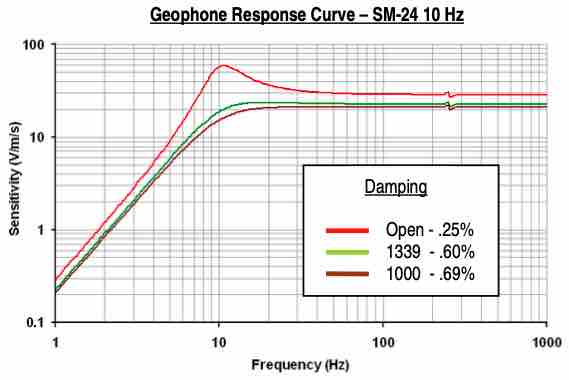
\includegraphics[scale = 0.7]{figures/seismic_graph.jpg}
\end{figure}

\begin{figure}[H]
  \centering
  \caption[Seismic sensor with 1k resistor.]{\emph{Seismic sensor with 1k resistor. }}\label{fig:seismic_res}
  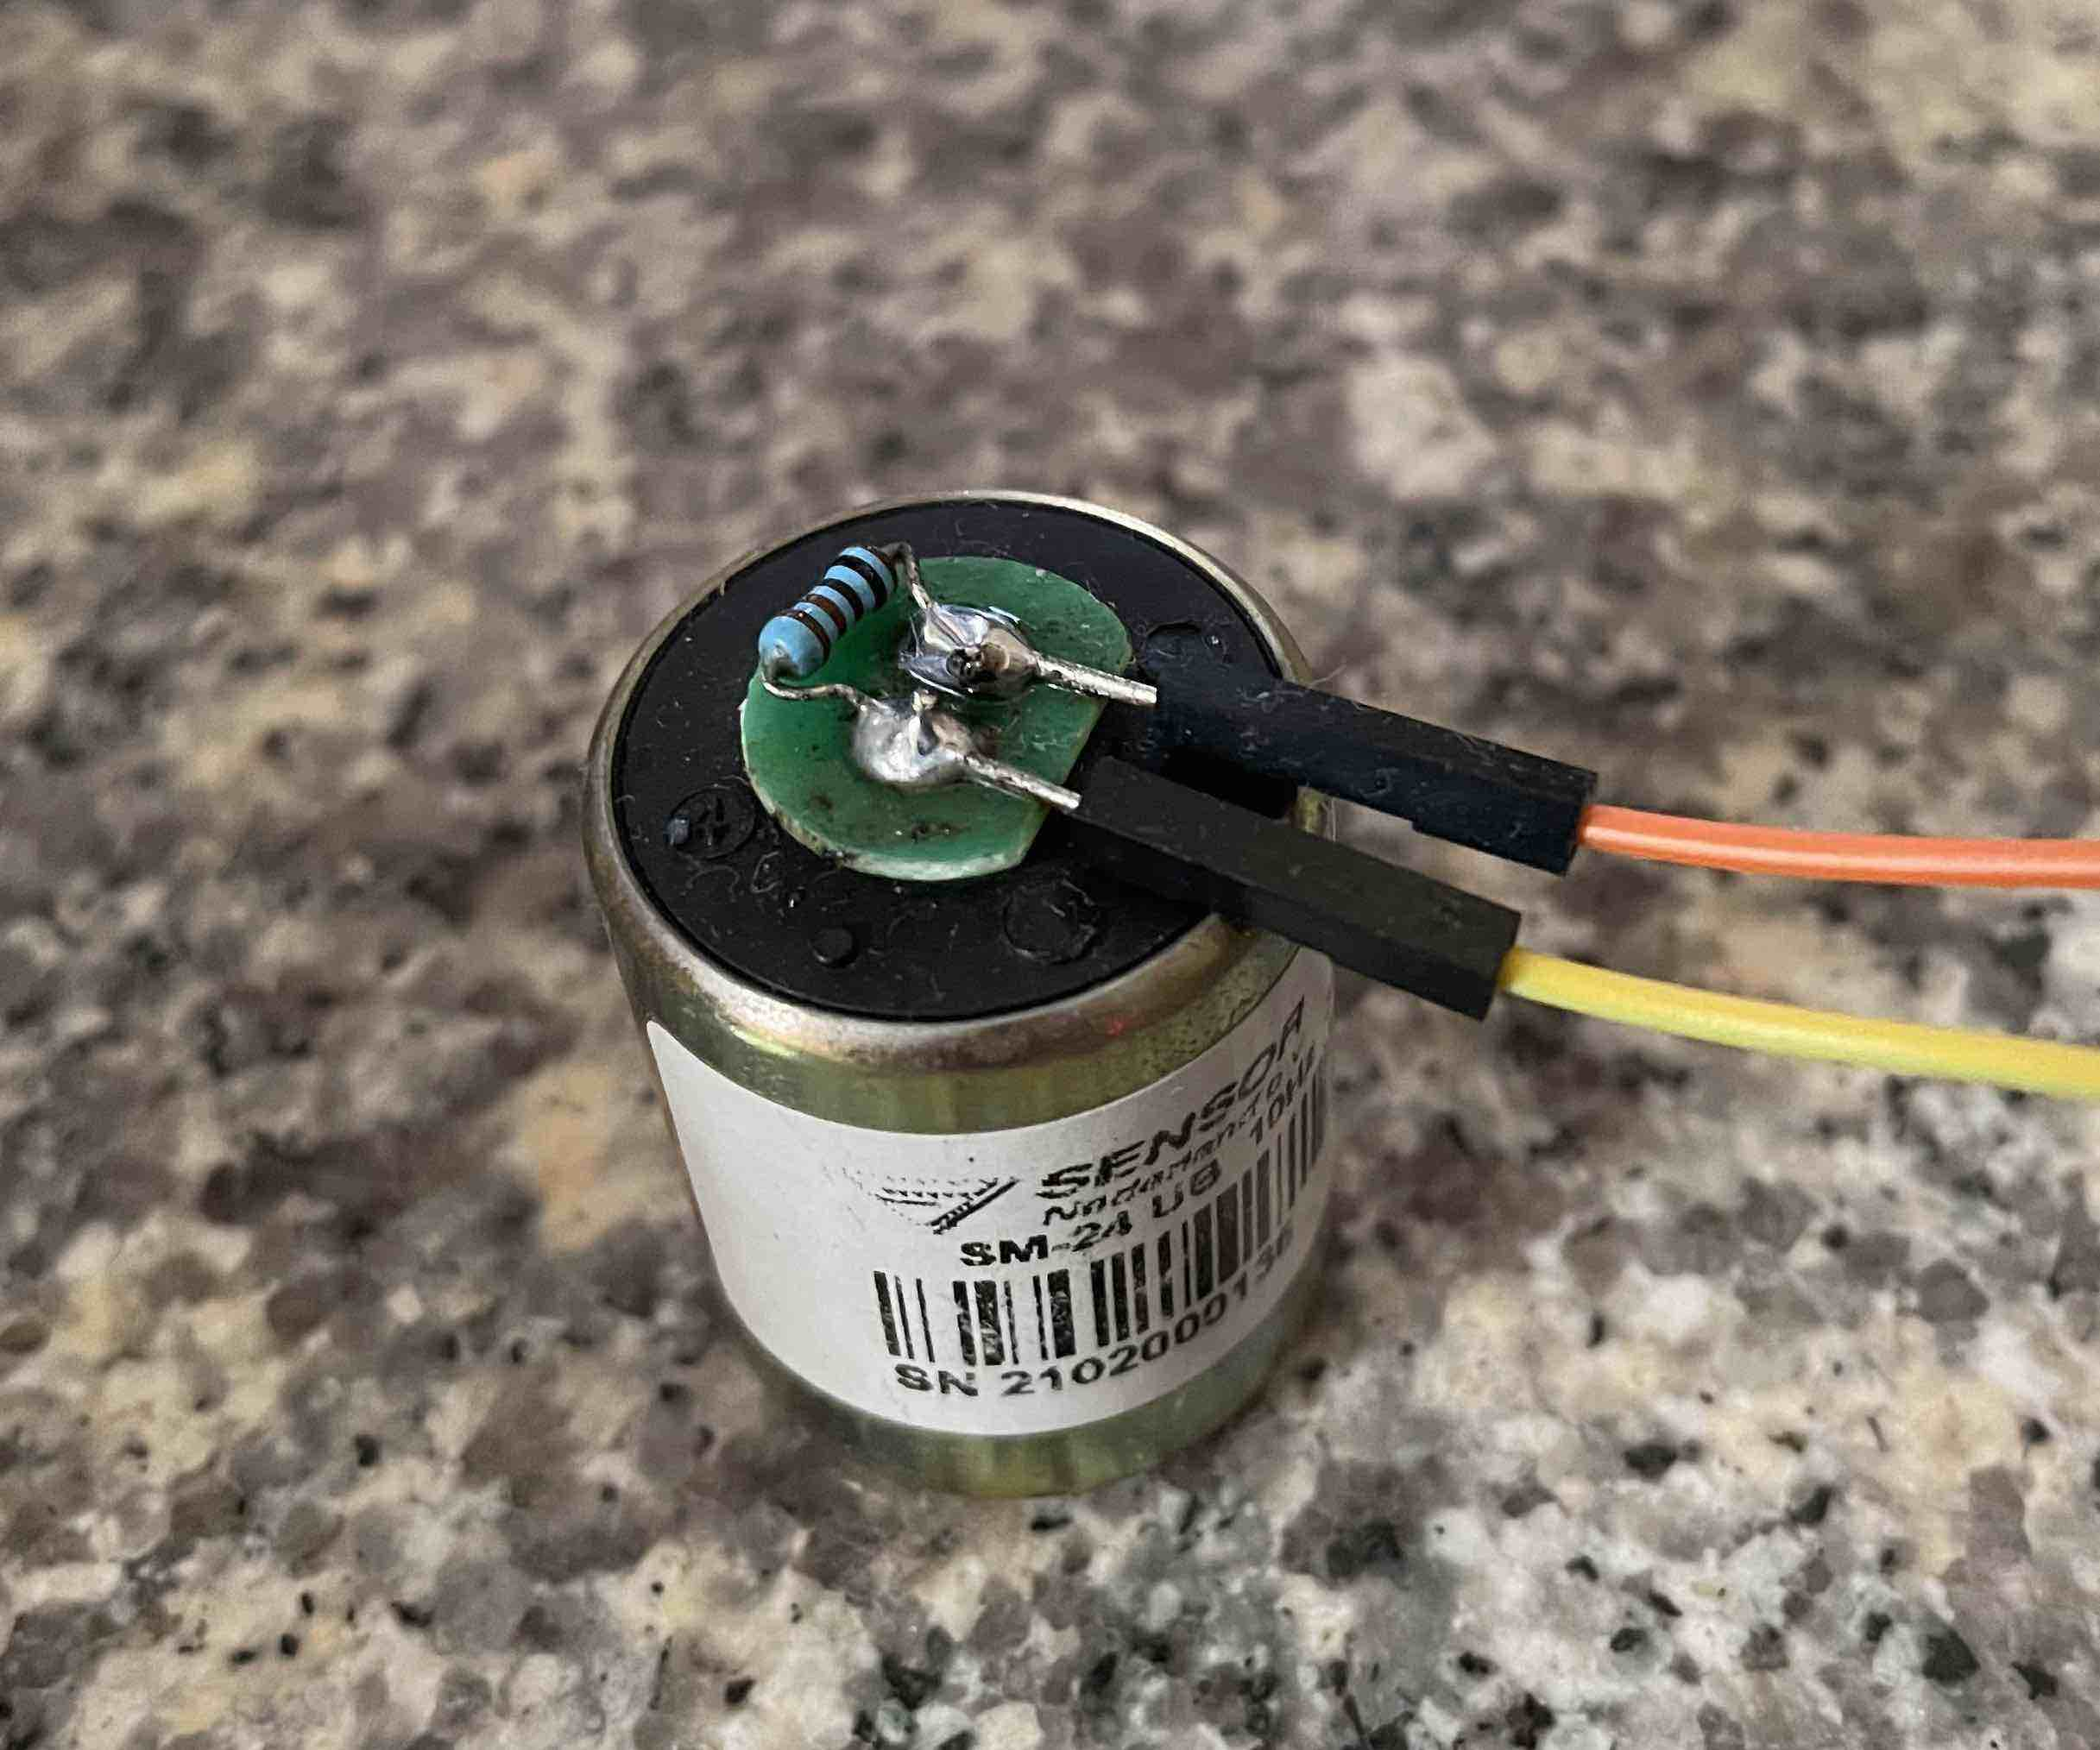
\includegraphics[scale = 0.13]{figures/seismic_res_low.jpg}
\end{figure}


The seismic sensor has a working range of 10 -- 240 Hz. Therefore, the analog filter circuit should implement a band-pass filter. We decided to use a non-inverting amplifier based band pass filter. The circuit components are shown in Figure \ref{fig:analog_circuit_}, and the circuit frequency response is shown in Figure \ref{fig:analog_circuit_cal}. We obtained an appropriate amplifier gain by a trial-and-error process at the AIT IoT lab. Once we were confident that the sensor and analog circuit could catch human activity signals within the range of the amplifier circuit output, i.e., 0-5 V, we designed and built the filter with an amplifier with voltage gain of : 400 V/V and a bandwidth : 1 -- 200 Hz. This amplifier gain is high because we need to extract information from faint vibrations due to human activity on the concrete floor. Lower amplifier gains make it very difficult to extract signal related to human activity. The physic of the complete data acquisition circuit is shown in Figure \ref{fig:physical_analog_circuit}.


The limitation of this data acquisition circuit is when these ranges are reached, some information cannot be extracted from sensor.


\begin{figure}[H]
  \centering
  \caption[Non-Inverting amplifier-based band Pass Filter.]{\emph{Non-Inverting amplifier-based band Pass Filter.}}\label{fig:analog_circuit_}
  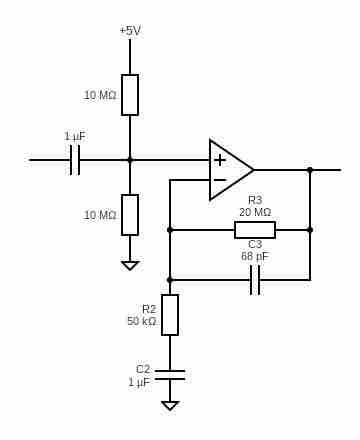
\includegraphics[scale = 0.7]{figures/analog_circuit_1.jpg}
\end{figure}

\begin{figure}[H]
  \centering
  \caption[Frequency response of non-inverting amplifier based band pass filter and formula.]{\emph{Frequency response of non-inverting amplifier based band pass filter and formula. 52 dB is equal to 400 V/V}}\label{fig:analog_circuit_cal}
  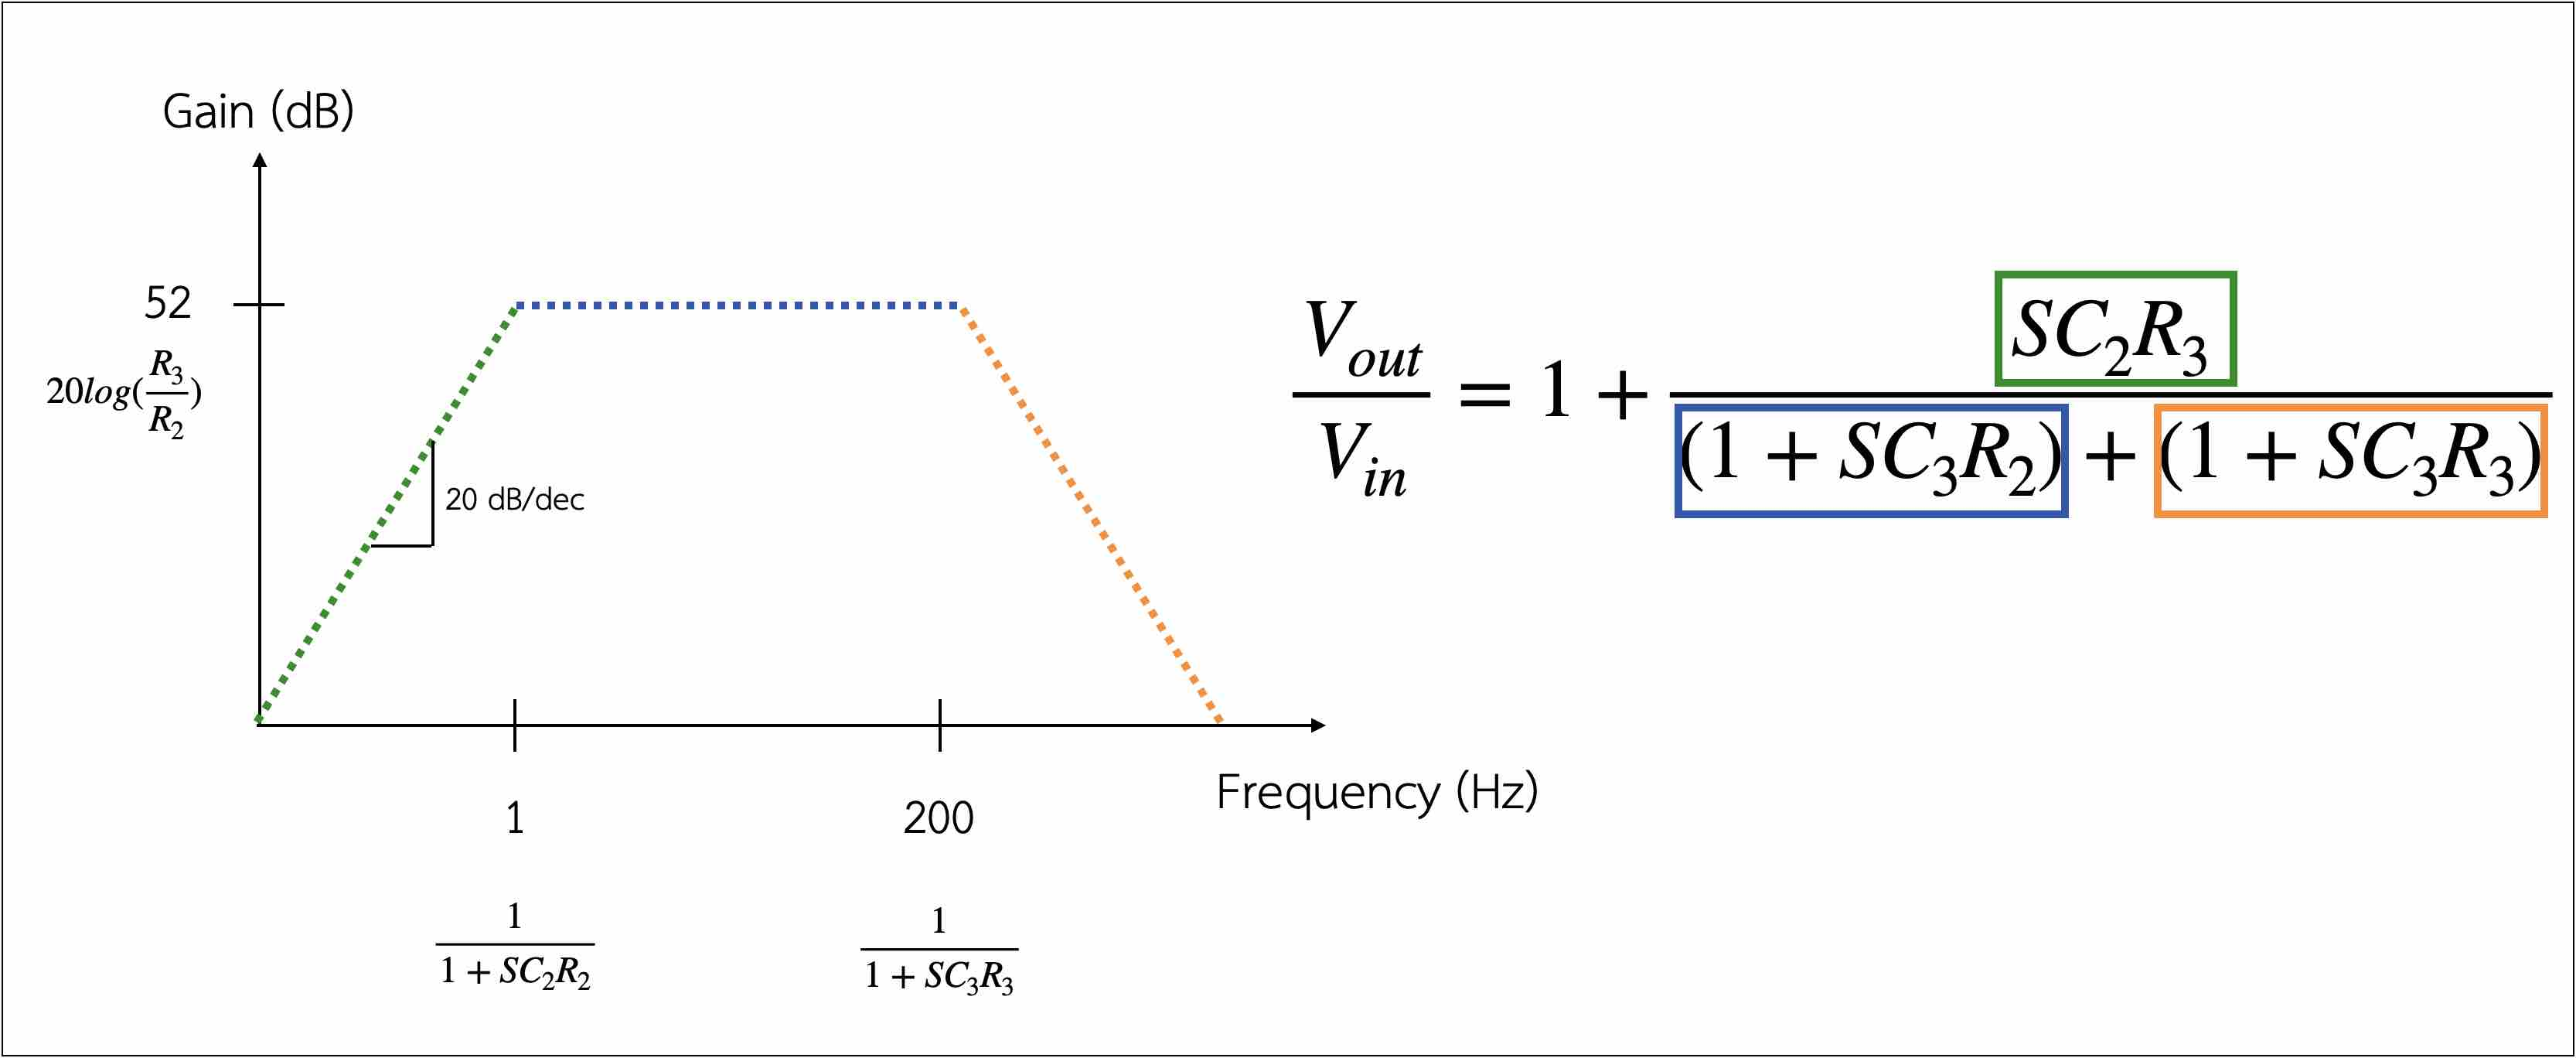
\includegraphics[scale = 0.15]{figures/analog_circuit_2.jpg}
\end{figure}

\begin{figure}[H]
  \centering
  \caption[The physical data acquisition circuit.]{\emph{The physical data acquisition circuit.}}\label{fig:physical_analog_circuit}
  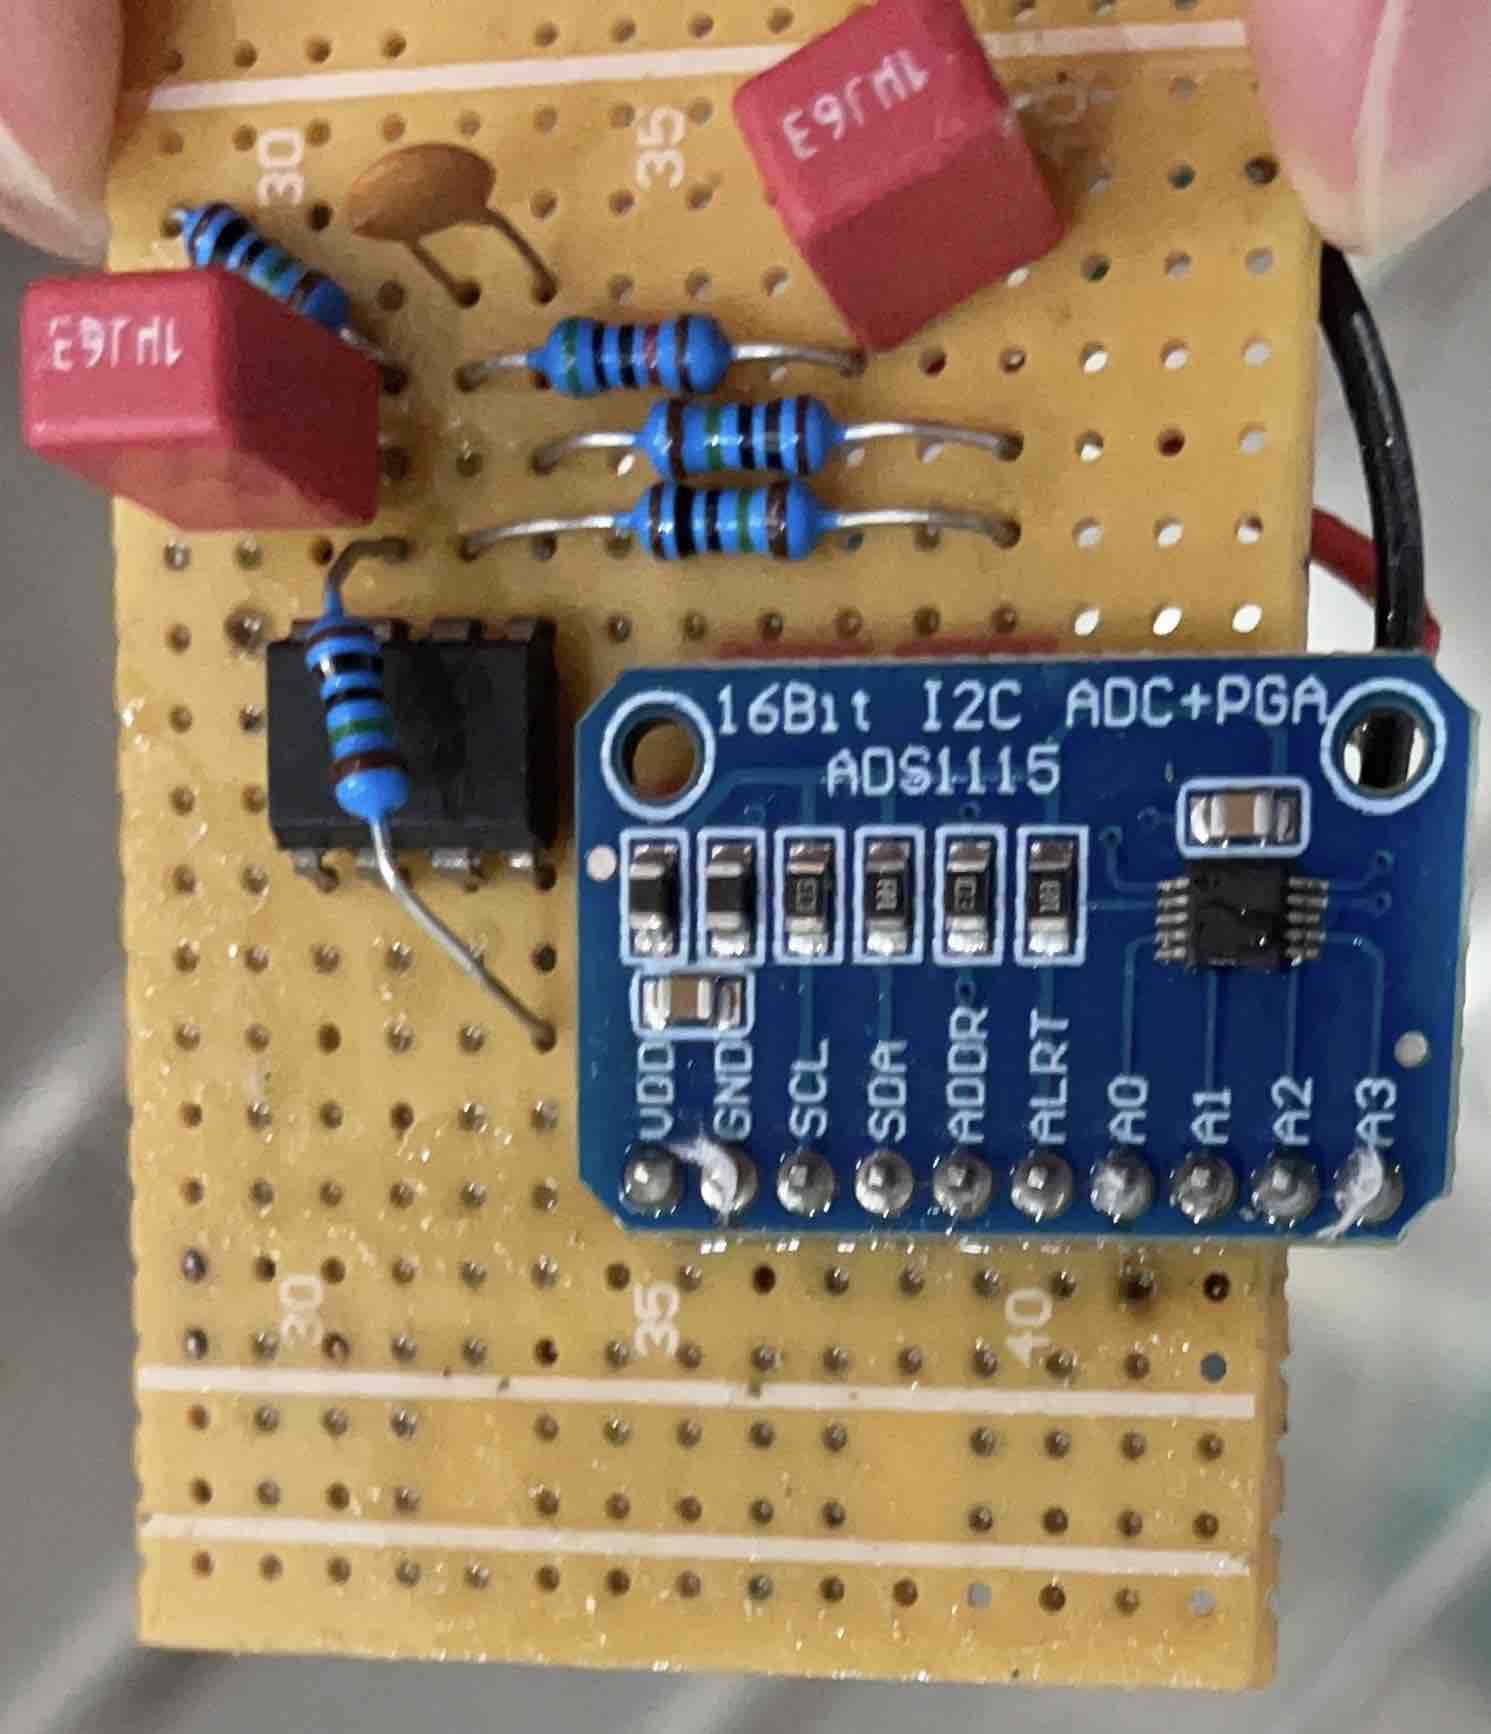
\includegraphics[scale = 0.15]{figures/physical_analog_circuit.jpg}
\end{figure}

\section{Collect data on daily human activities by many subjects.}
\subsection{Experimental Setup}


To collect the raw data, I performed experiments in the living room of my house in Bangkok, Thailand, which was built from reinforced concrete with tile, as shown in Figure \ref{fig:home}. The system can detect vibrations in a range of around five meters, and the room has dimension 3.5 m $\times$ 3.5 m, so one sensor unit is sufficient to extract humana activity signals occuring within the room. The hardware should be installed near a corner of the room in order to be as suitable for the application as possible.

\begin{figure}[H]
  \centering
  \caption[Living room area used for preliminary experiment.]{\emph{Living room area used for preliminary experiment.}}\label{fig:home}
  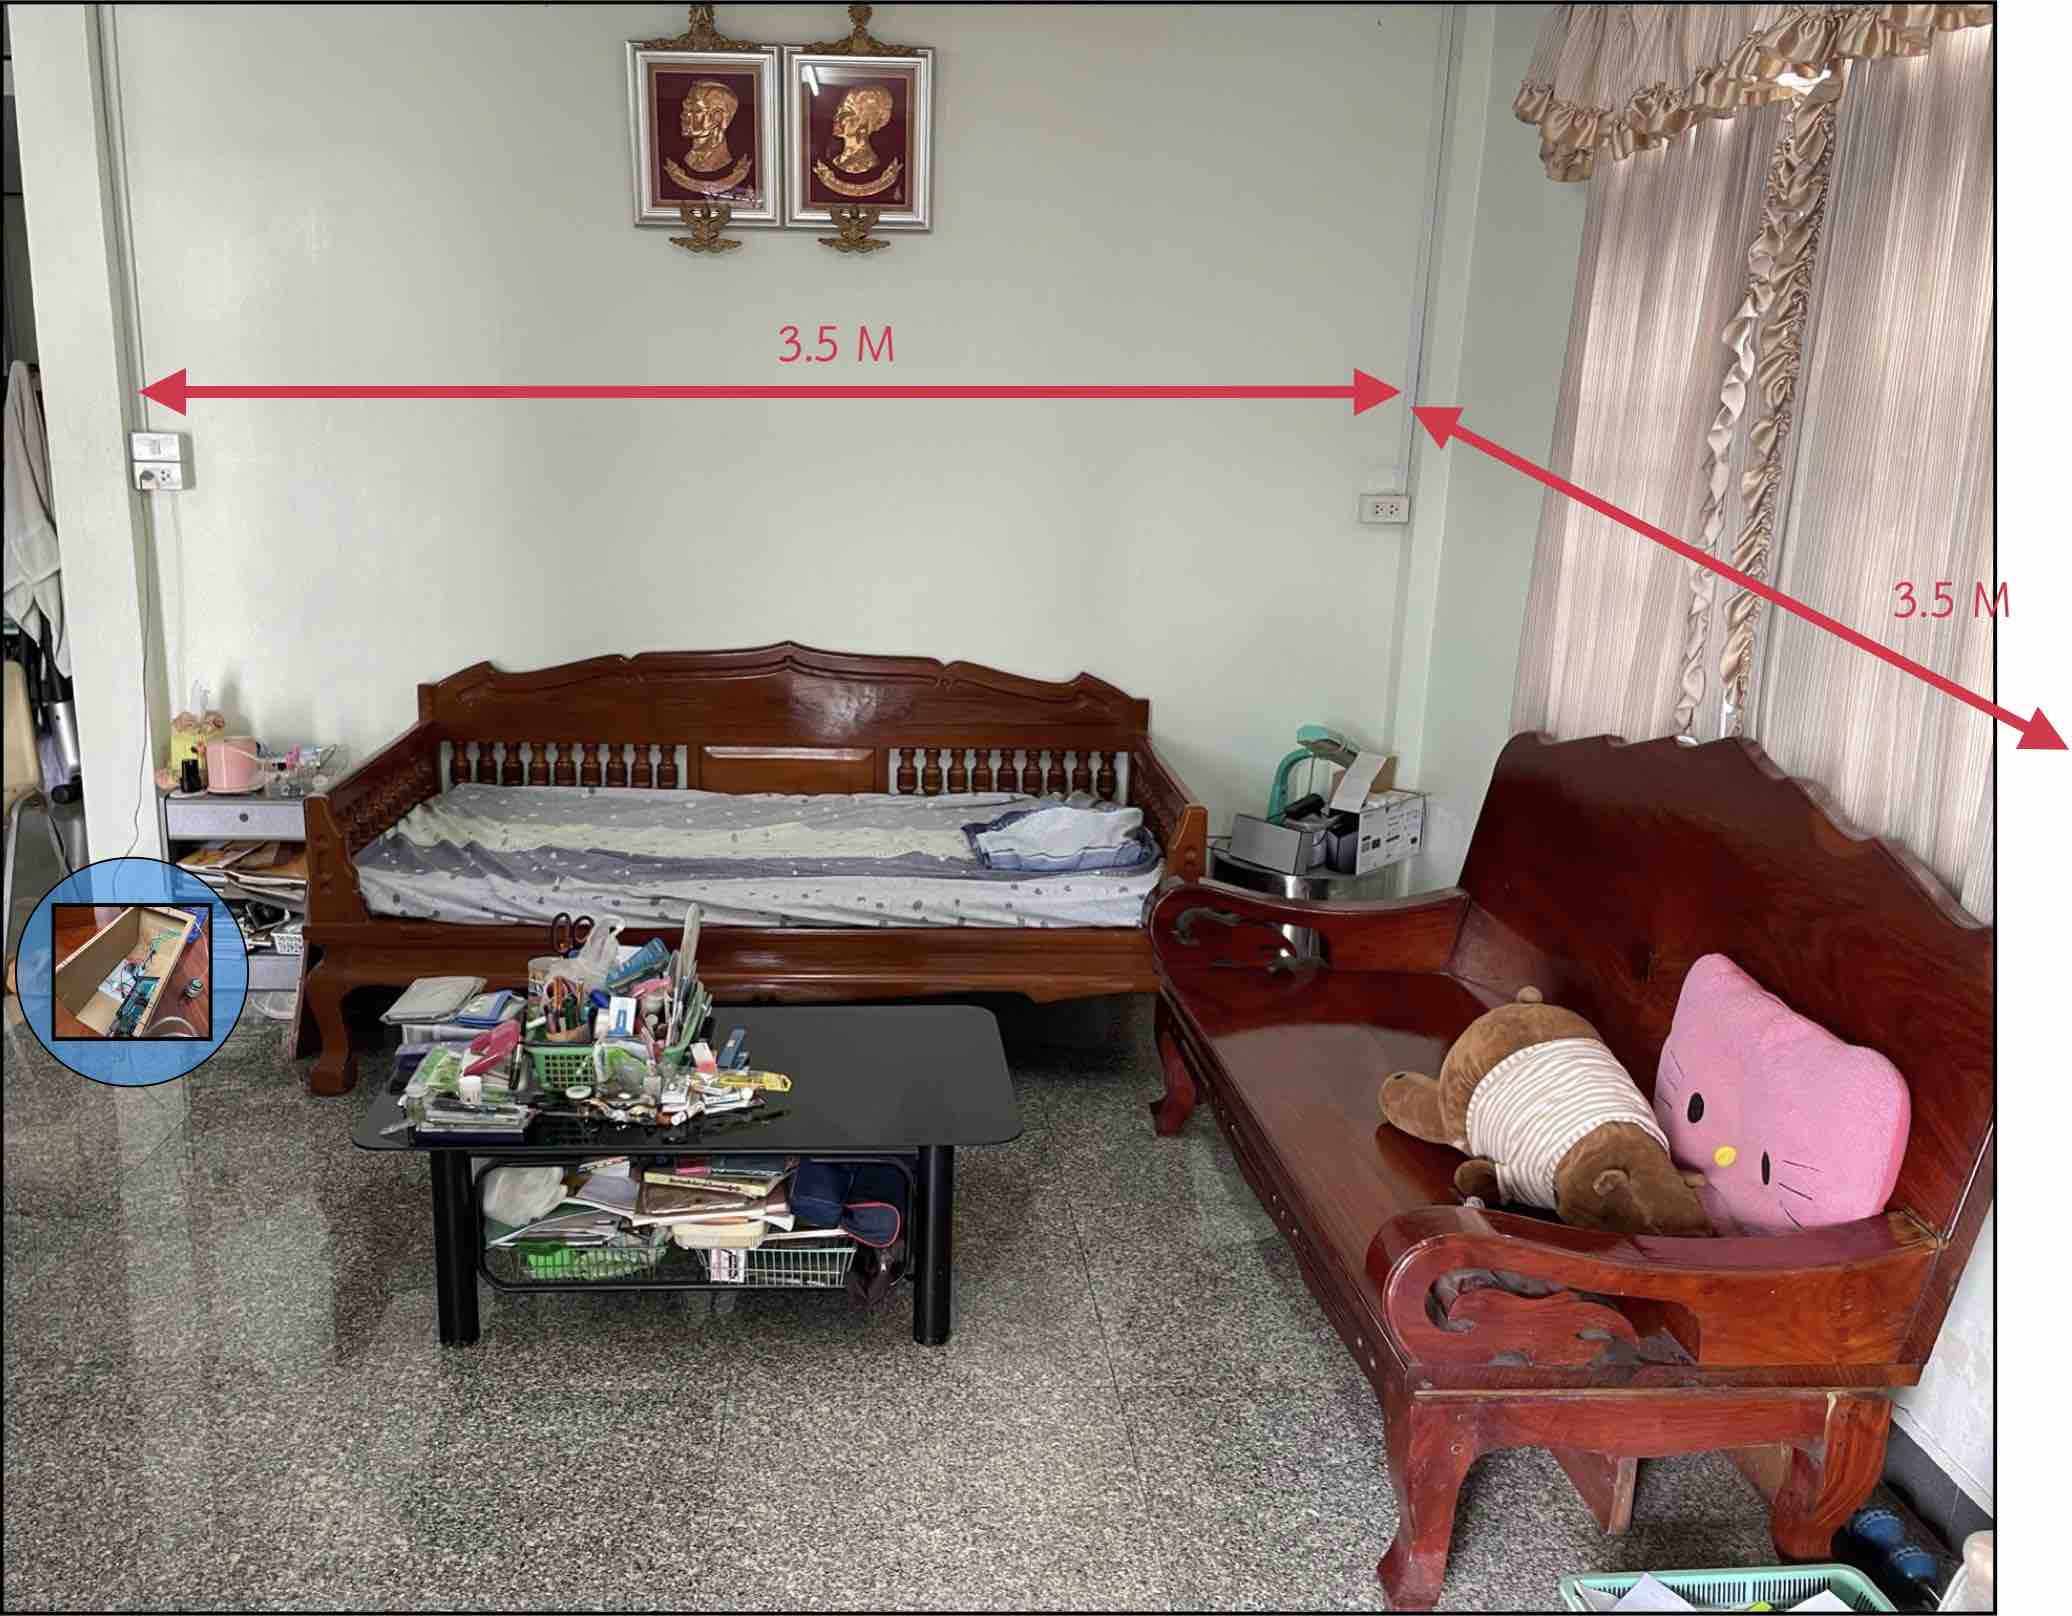
\includegraphics[scale = 0.2]{figures/home.jpg}
\end{figure}


\subsection{Ordinary activities}

There are several activities that occur normally during daily life. I focus on typical activities such as walking, sitting, standing and lying down, as shown in Table \ref{tab:number_action}. Under COVID-19, since I cannot invite outside volunteers to come indoor for data collection, I collected activities of four subjects, my father, my mother, my older brother, and me. Details of participants are shown in Table \ref{tab:participants}.

\begin{table}[H]
  \begin{center}
    \caption[Frequence of each ordinary activity.]{\emph{Frequence of each ordinary activity.} \\ \hspace{\textwidth}}\label{tab:number_action}
    \begin{tabular}{ l r }
      \textbf{Human Activity} & \textbf{Number of action} \\
      \hline
      Walking                 & 2,500                     \\
      \hline
      Sitting                 & 400                       \\
      \hline
      Standing                & 400                       \\
      \hline
      Lying                   & 400                       \\
      \hline
    \end{tabular}
  \end{center}
\end{table}

\begin{table}[H]
  \begin{center}
    \caption[Participant characteristics.]{\emph{Participant characteristics.}
      \\ \hspace{\textwidth}}\label{tab:participants}
    \begin{tabular}{c c c c}
      \textbf{Subject} & \textbf{Sex} & \textbf{Age} & \textbf{Weight $(kg)$} \\
      \hline

      1                & M            & 23           & 58                     \\
      \hline

      2                & M            & 25           & 70                     \\
      \hline

      3                & M            & 55           & 70                     \\
      \hline

      4                & F            & 58           & 75                     \\
      \hline
    \end{tabular}
  \end{center}
\end{table}


\subsection{Abnormal activities}

To understand the system's ability to highlight abnormal events, we need activities that rarely occur in normal daily life, such as jumping and dropping a 1.5 liter bottle of water (from different height levels) in random locations within the living room to ensure that regardless of the location of event, this system can detect the anomalous activities.

\subsection{Data folder architecture}

We do not only collect data for the current system, but we also would like others who are interested to futher develop the system to use our data. The folder structure is shown in Figure \ref{fig:folder}. On the main branch, each folder contains the activity details of each subject. Inside the activity folders, there are two folders, ``Raw'' containing raw data from the sensor, and ``Clean'' containing cleaned data that have been prepocessed (details are explained in next section). Anyone can access the data at \url{https://drive.google.com/drive/folders/1ZZjKl8cD5dTt1JukgNvjxWVY45wiKq6o?usp=sharing}.

\begin{figure}[H]
  \centering
  \caption[The folder structure for open dataset.]{\emph{The folder structure for open dataset.}} \label{fig:folder}
  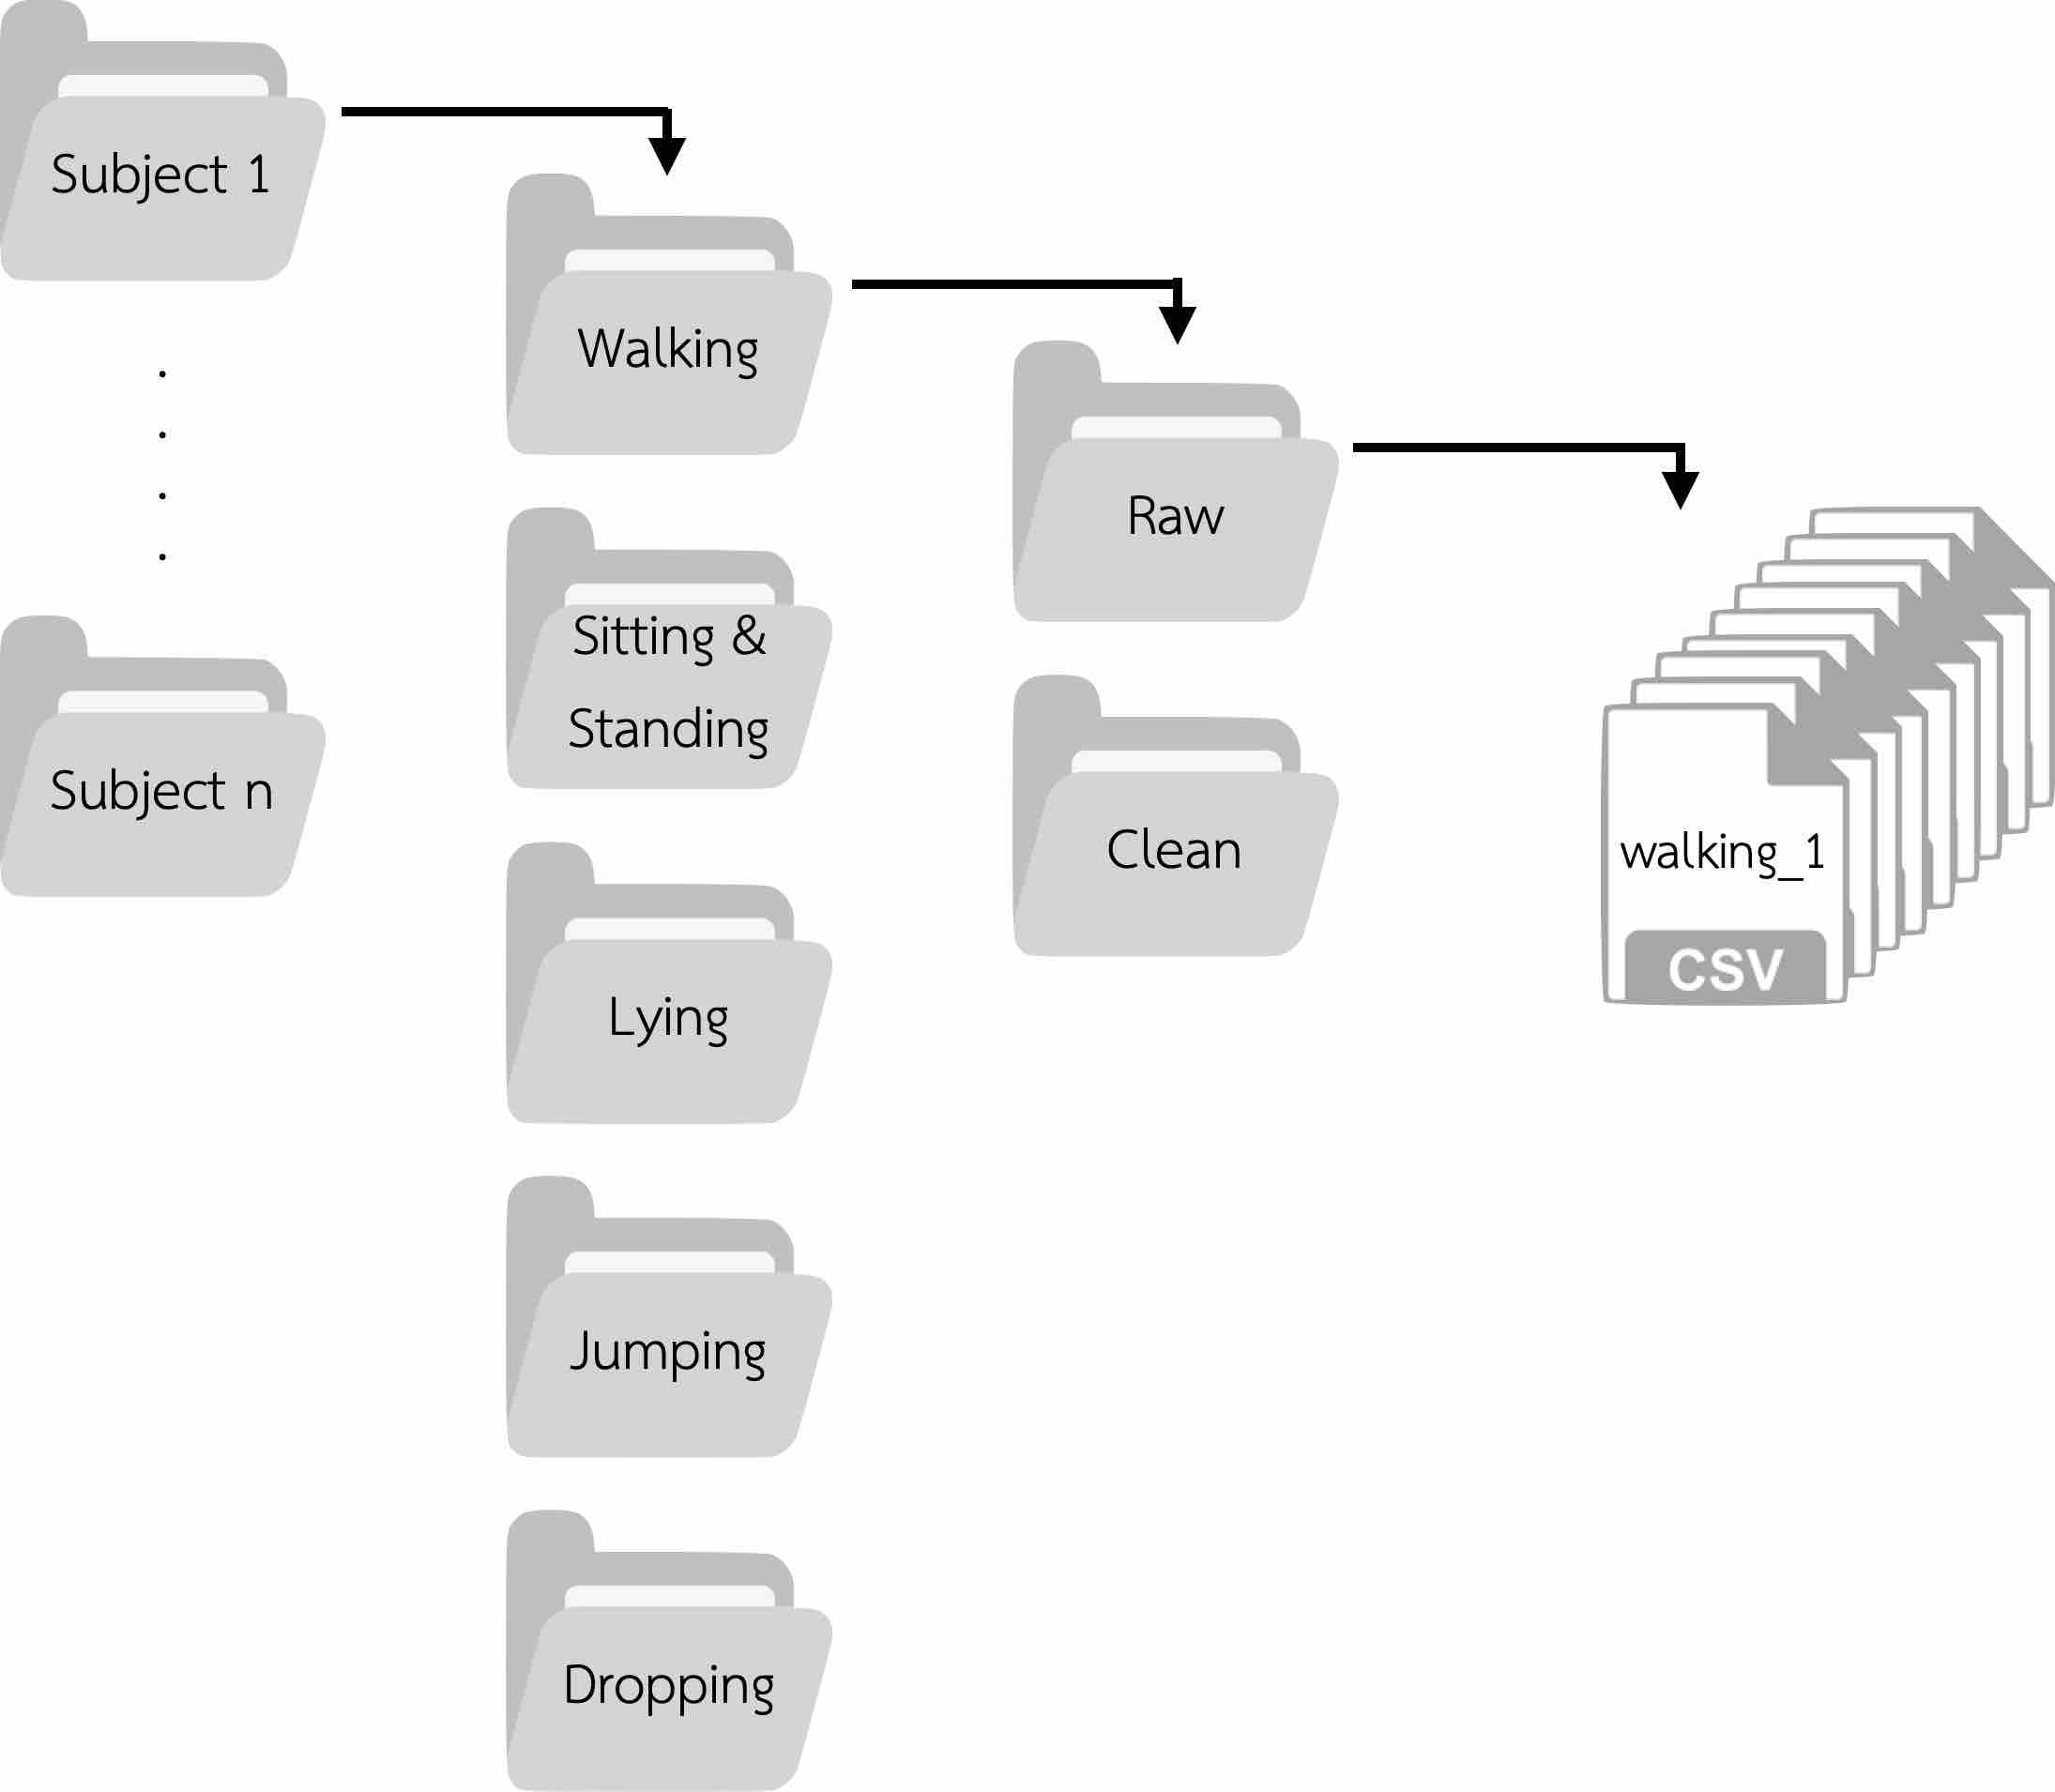
\includegraphics[scale = 0.15]{figures/data_architecture.jpg}
\end{figure}

\section{Build anomaly detection models likely to detect fall as anomalies}

The machine learning process is shown in Figure \ref{fig:work-flow}. The raw data cannot be fed directly to the model, because they contains power system noise. We therefore need to preprocess them first.

\begin{figure}[H]
  \centering
  \caption[Machine learning process.]{\emph{Machine learning process.}} \label{fig:work-flow}
  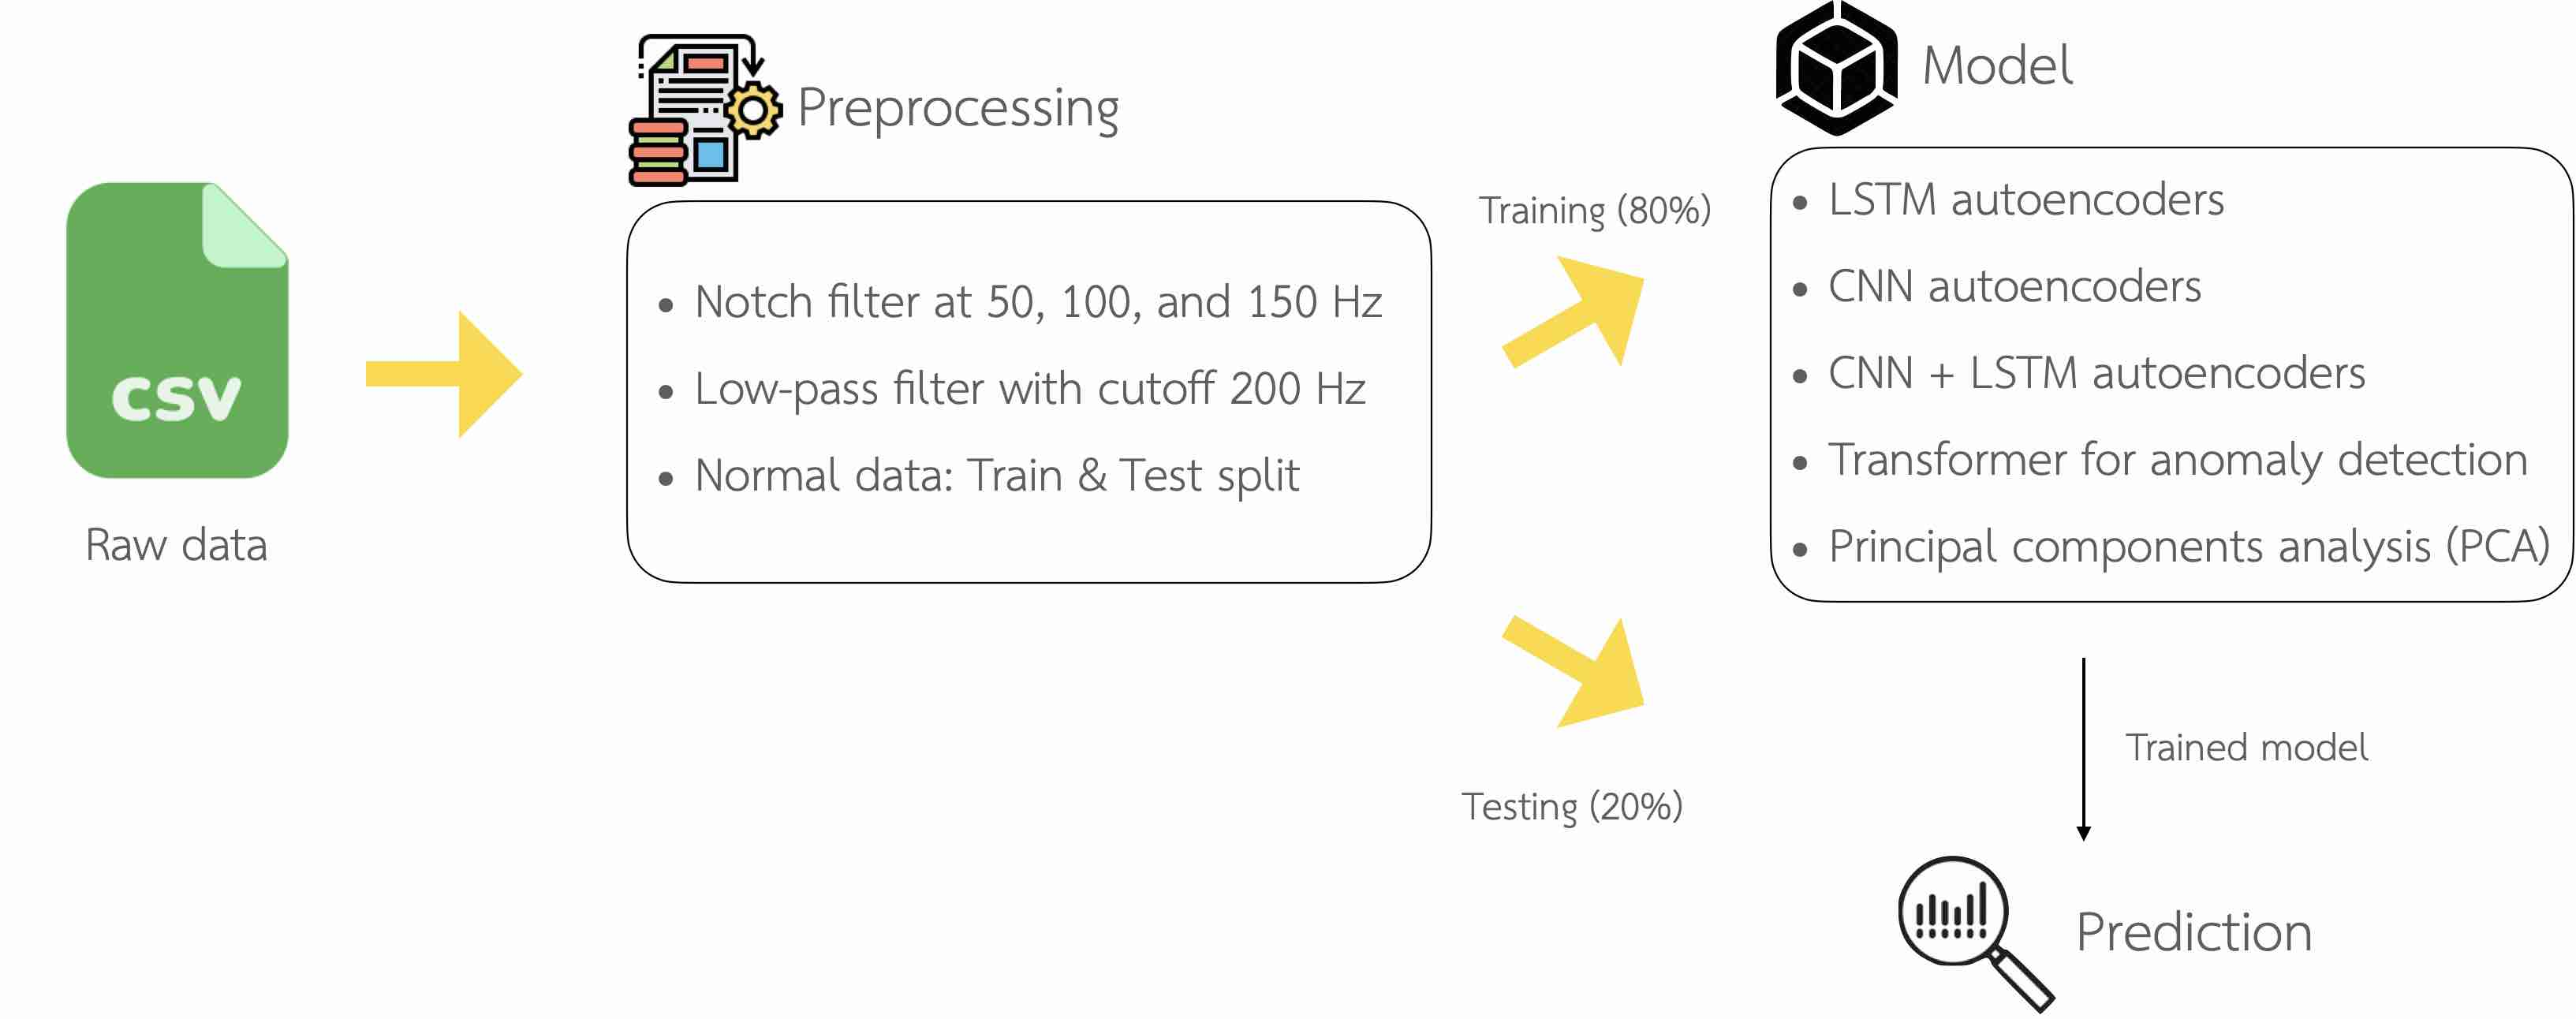
\includegraphics[scale = 0.13]{figures/work-flow.jpg}
\end{figure}


The need for prepocessing is examplified in the frequency domain profiles of a walking activity with and withiut a common earth ground as shown in Figure \ref{fig:fft_raw_data}. The upper image is the preferred signal recorded with an isolated ground provided by an oscilloscope. The lower image shows an actual signal collected without an isolated ground in a real home environment. There is clearly some AC coupling, resulting in spikes at 50 Hz, 100 Hz, 150 Hz, and so on. This problem may be exacerbated by the high amplifier gain used in the analog circuit. In order to allow convenient use of the system in an ordinary home, we apply a notch filter to the signal. We pass the signal though three notch filters at 50 Hz, 100 Hz, and 150 Hz. Figure \ref{fig:notch_filter} shows the outcome of each state of notch filter. Then we also add a low-pass filter with cutoff frequency at 200 Hz in order to be compatible with analog filter and we would like to ensure that all of information are in range 1 -- 200 Hz. The cleaned data for each event are shown in Figure \ref{fig:cleaned_data}. All of the evidence mentioned above proves why we need to add notch and low-pass filters.


\begin{figure}[H]
  \centering
  \caption[Ideal frequency domain profile of walking signal.]{\emph{Ideal frequency domain profile of walking signal (top) recorded with a common earth ground vs. the actual frequency domain profile (bottom) recorded without a common earth ground.}} \label{fig:fft_raw_data}
  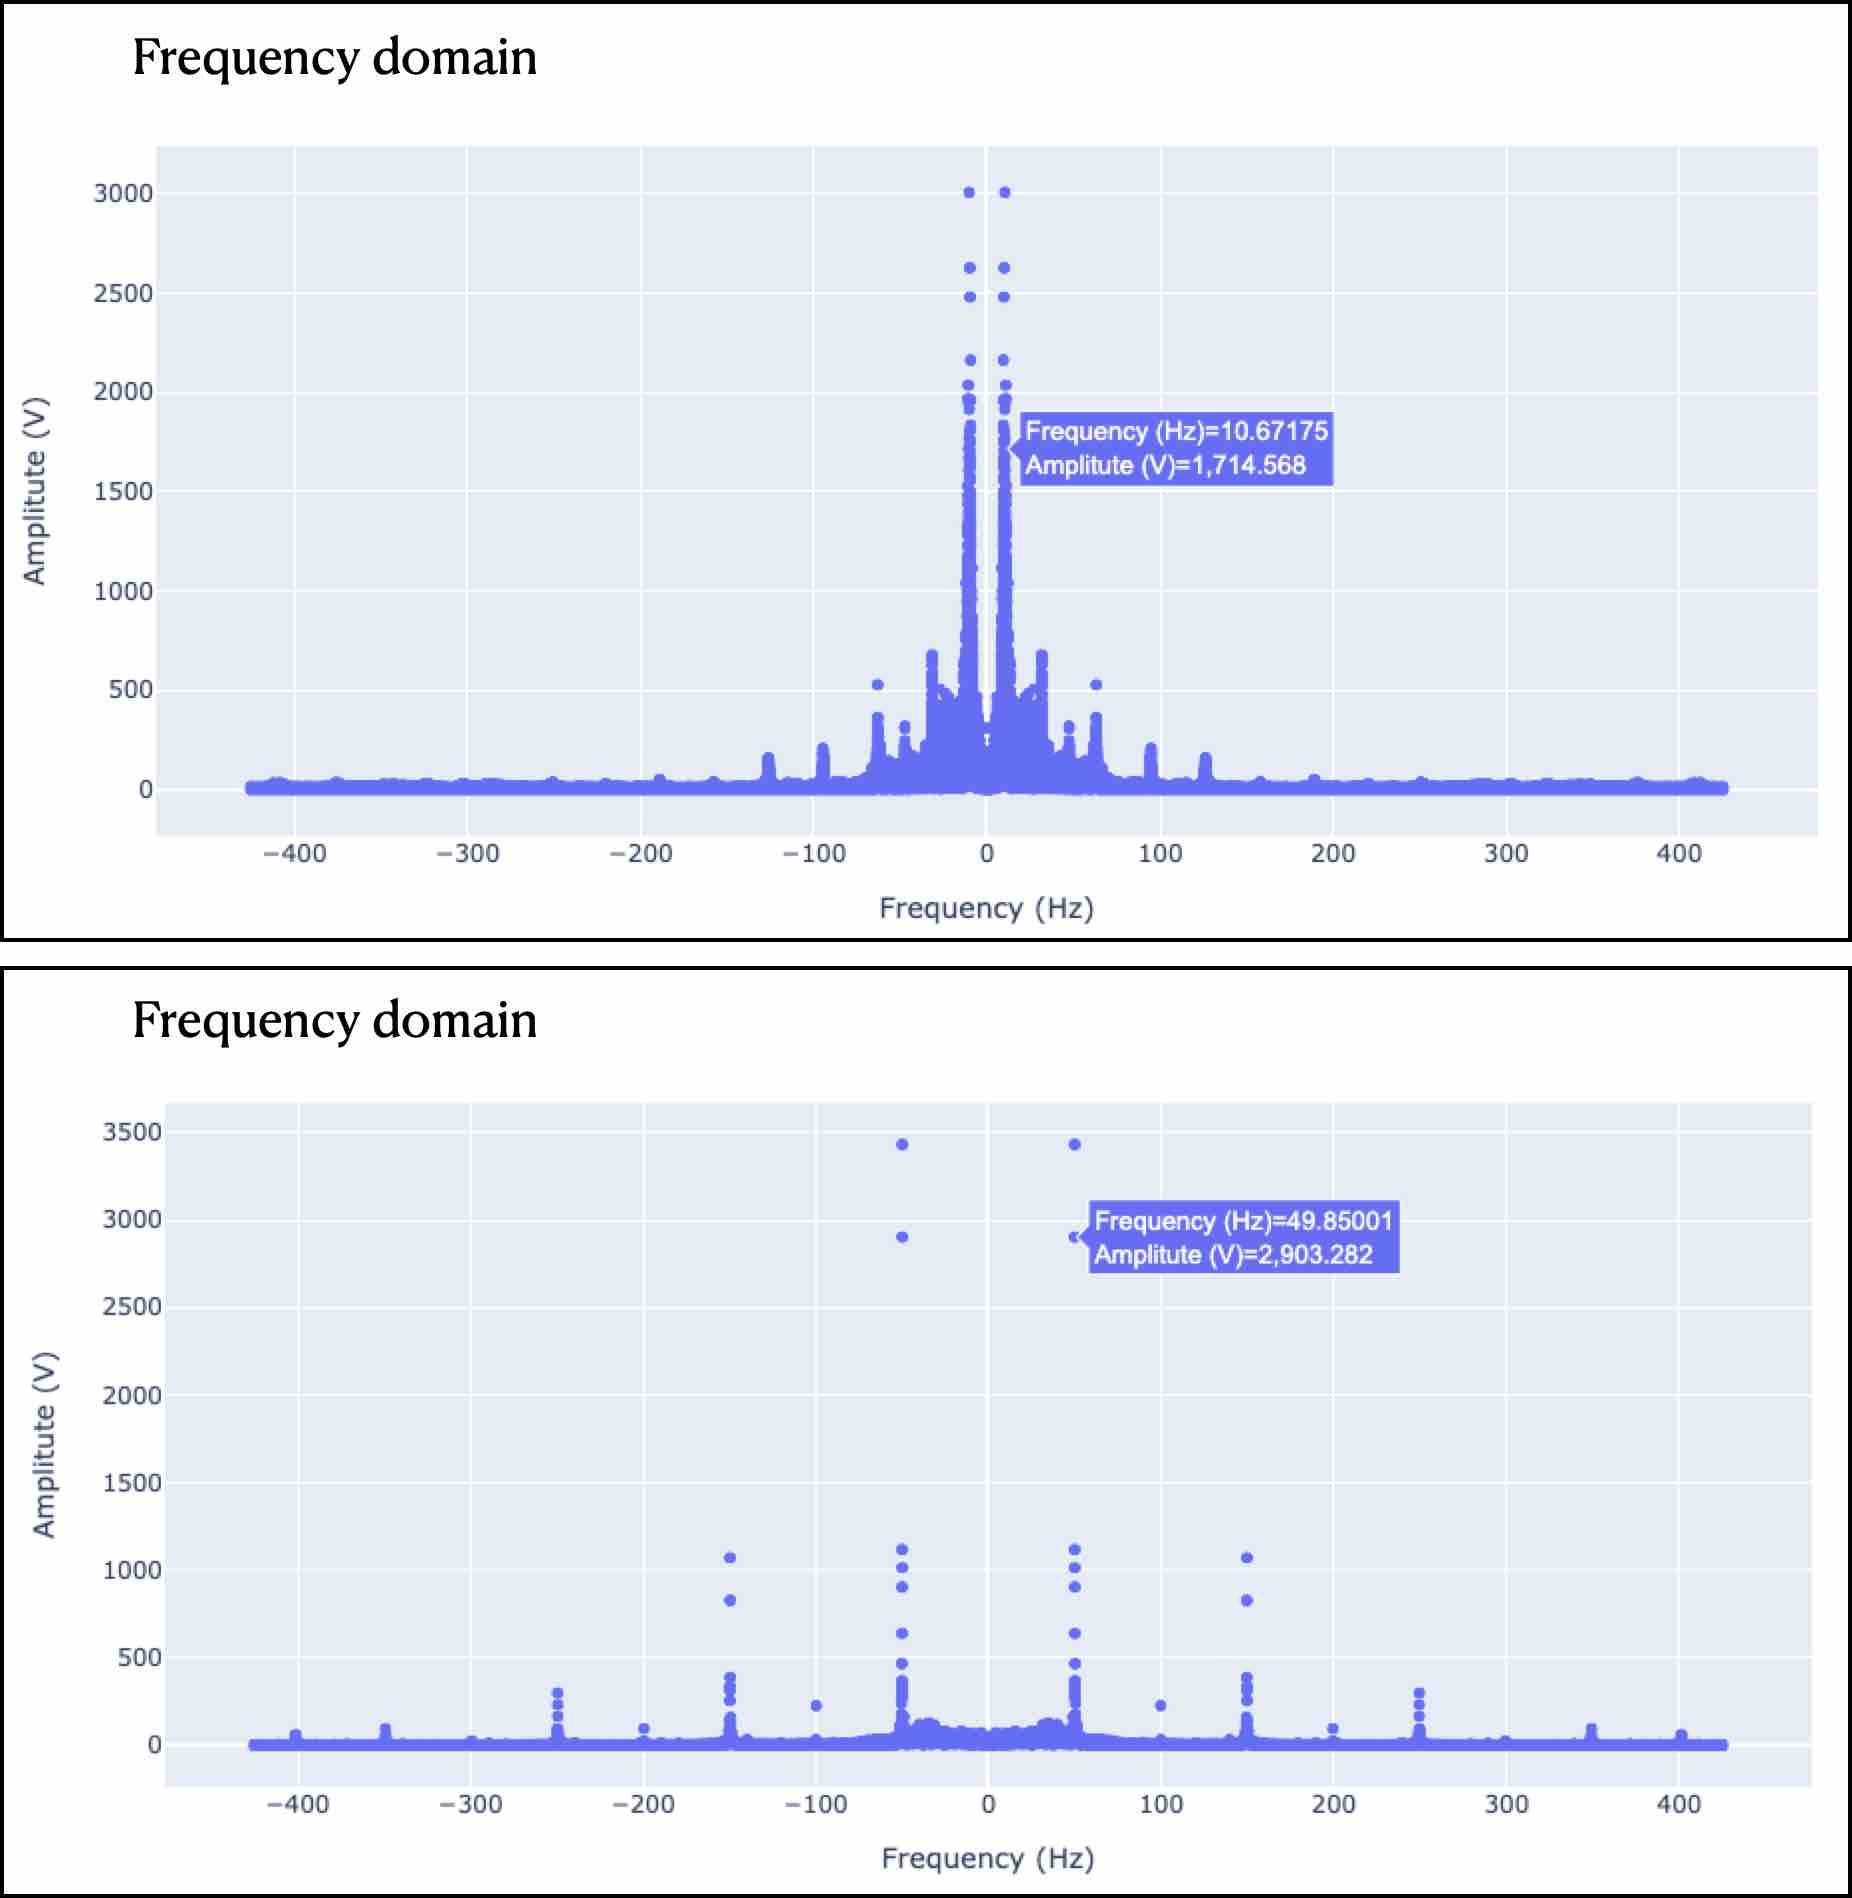
\includegraphics[scale = 0.22]{figures/fft_raw_data.jpg}
\end{figure}

\begin{figure}[H]
  \centering
  \caption[Output signal after prepocessing with each notch filter.]{\emph{Output signal after prepocessing with each notch filter.}} \label{fig:notch_filter}
  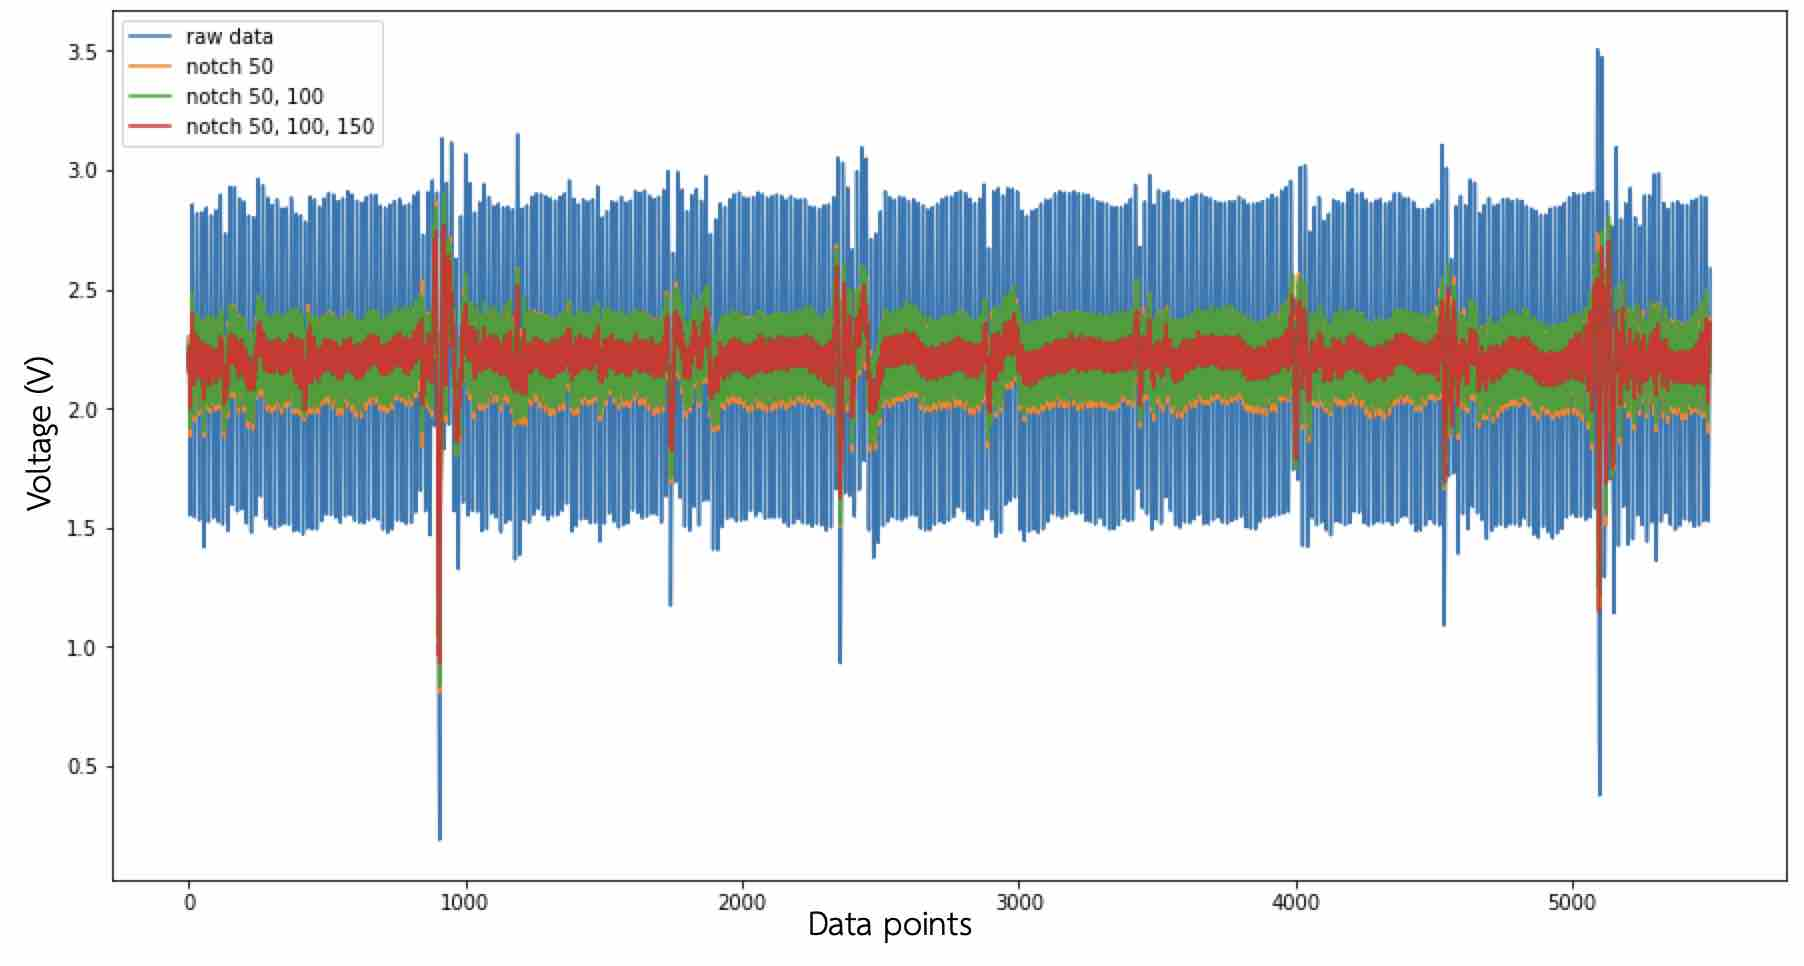
\includegraphics[scale = 0.22]{figures/notch_filter.jpg}
\end{figure}

\begin{figure}[H]
  \centering
  \caption[Samples of cleaned data for each event.]{\emph{Samples of cleaned data for each event.}} \label{fig:cleaned_data}
  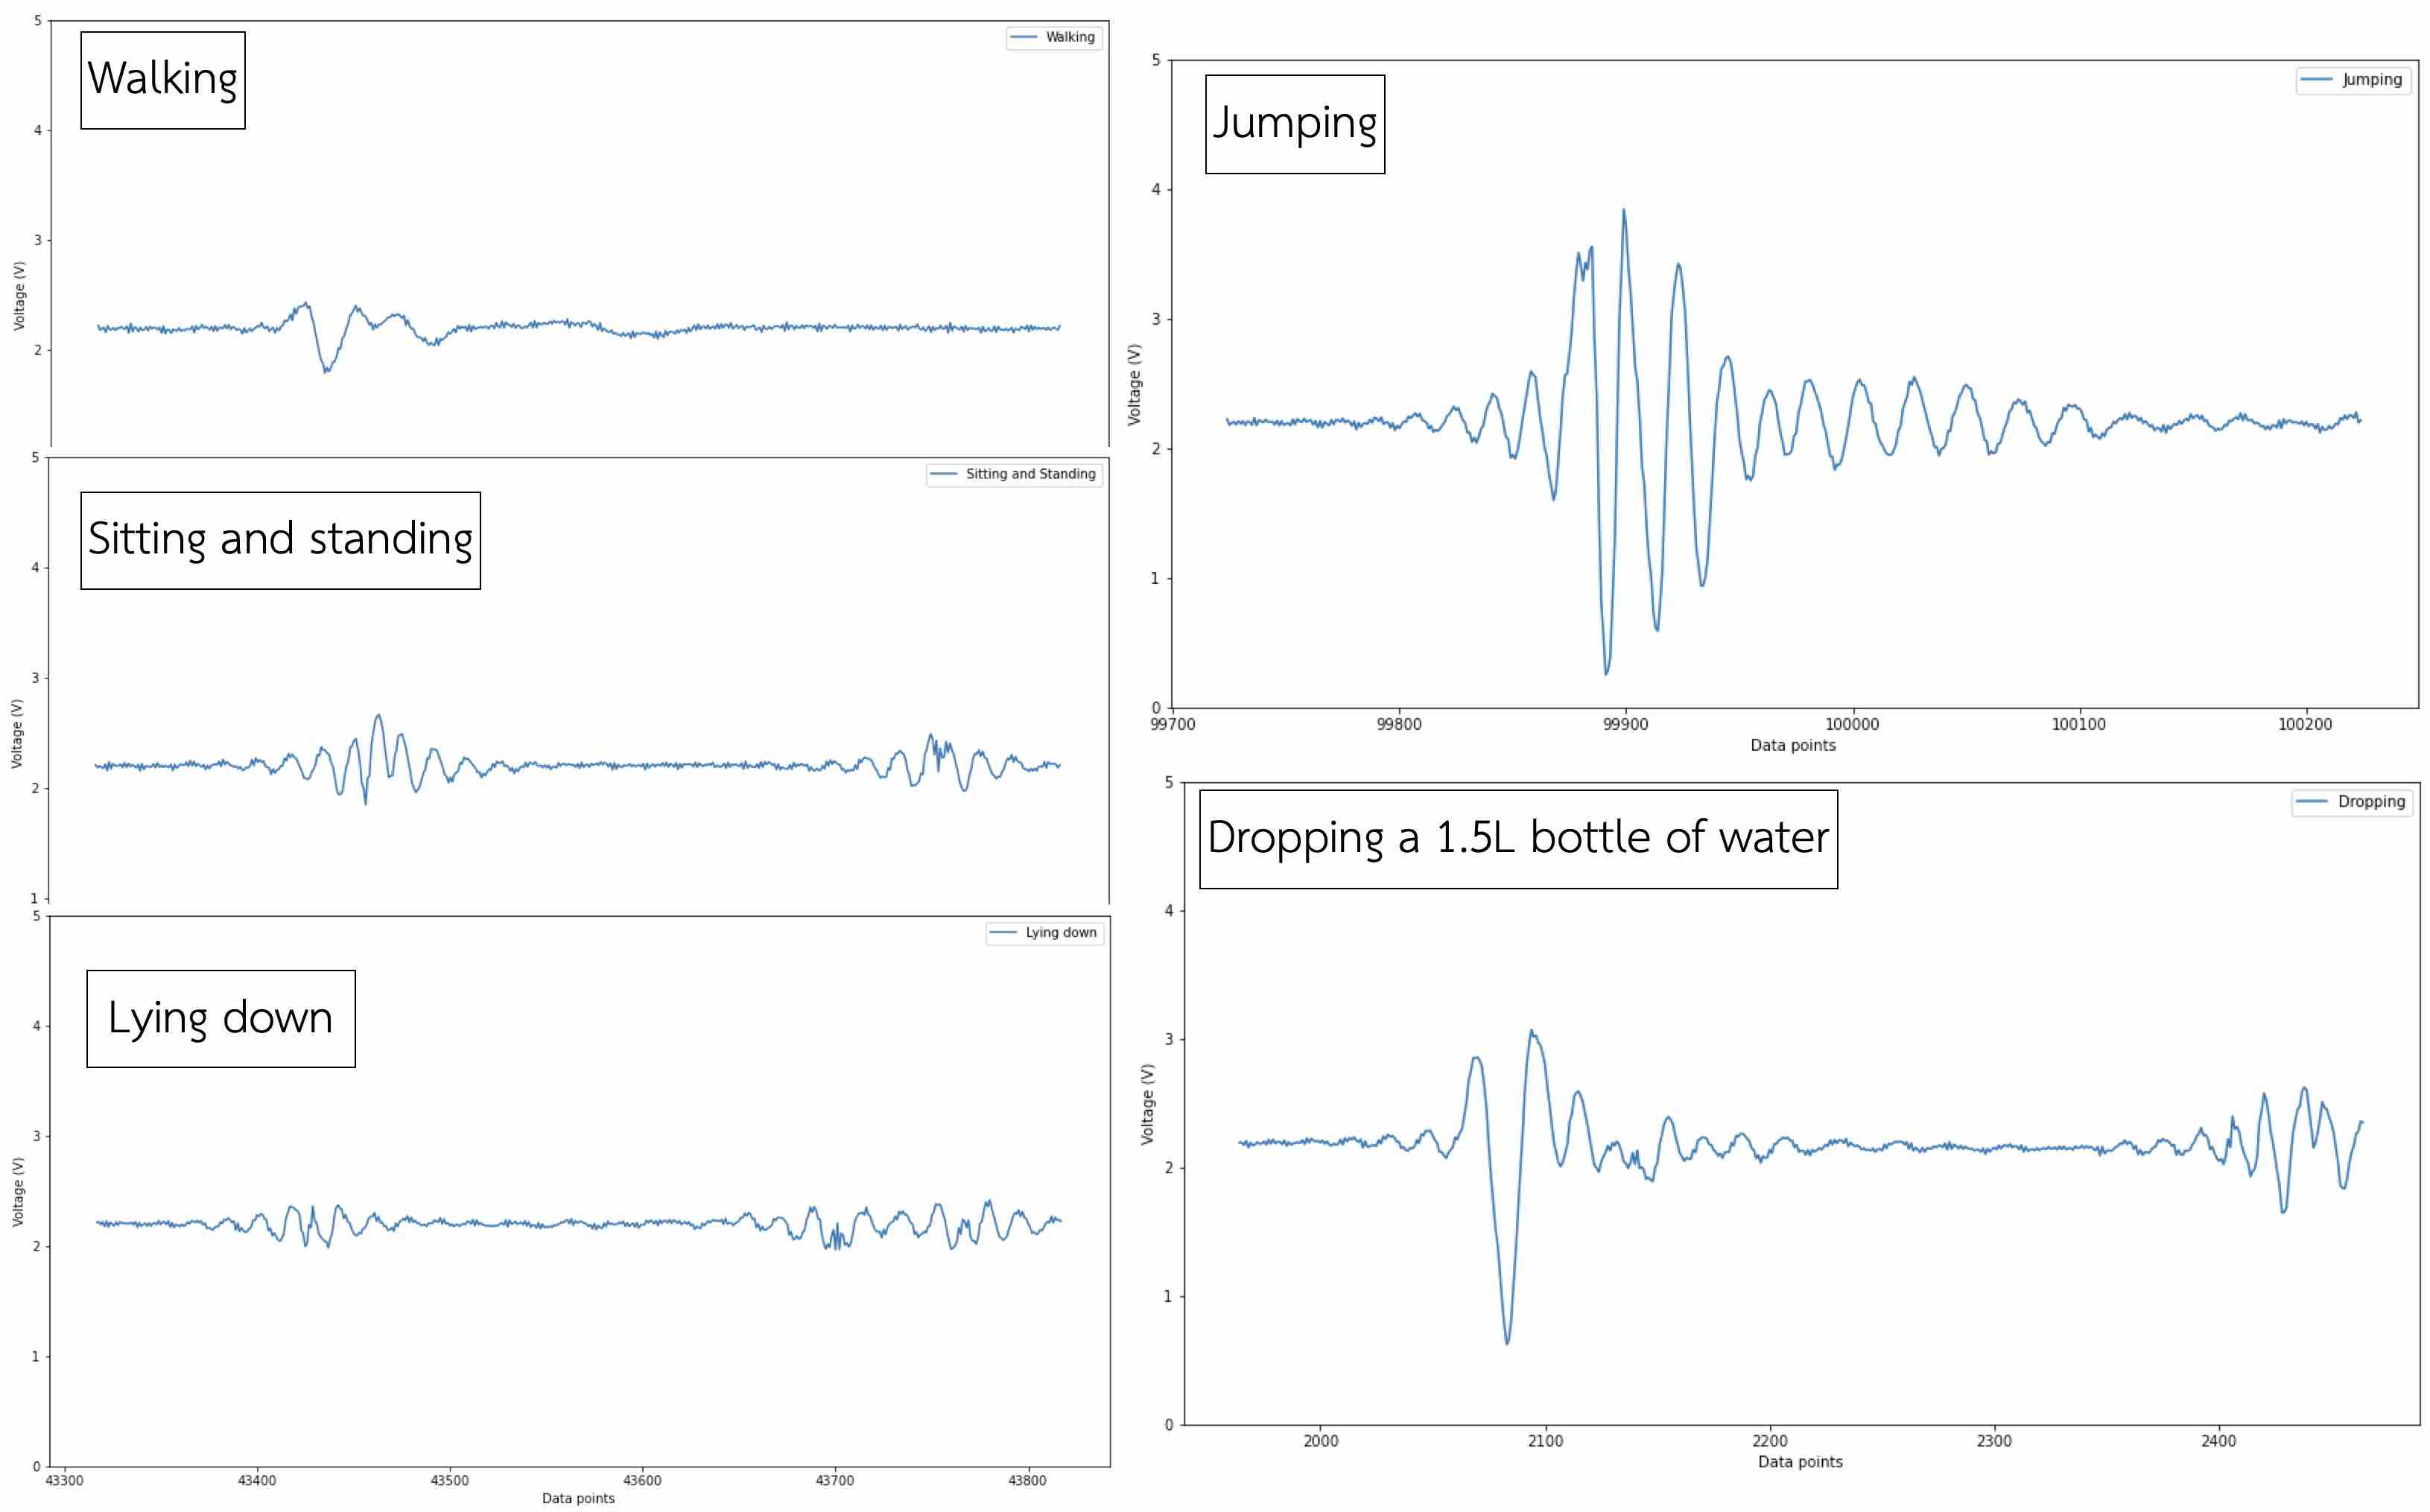
\includegraphics[scale = 0.15]{figures/cleaned_data.jpg}
\end{figure}

Given a cleaned signal for an event, in the machine learning model, we apply two main catagories of algorithms: deep learning models and traditional algorithms. Among the deep learning methods, we apply four models, an autoencoder with LSTM, a convolutional autoencoder, a convolutional autoencoder with LSTM, and a Transformer, for anomaly detection proposes. The four architectures are shown in Figures \ref{fig:autoencoder_lstm}, \ref{fig:autoencoder_cnn}, \ref{fig:autoencoder_cnnlstm} , and \ref{fig:transformer_1} respectively. We observe that the structures are quite similar in that they first pass sequential data though encoder modules and then transform the data back to the original dimensionality in decoder modules. The detailed configuration parameters and performance of each model are explained below. As a traditional algorithm, we apply principal components analysis (PCA).

\begin{figure}[H]
  \centering
  \caption[Anomaly detection autoencoder with LSTM architecture.]{\emph{Anomaly detection autoencoder with LSTM architecture.}} \label{fig:autoencoder_lstm}
  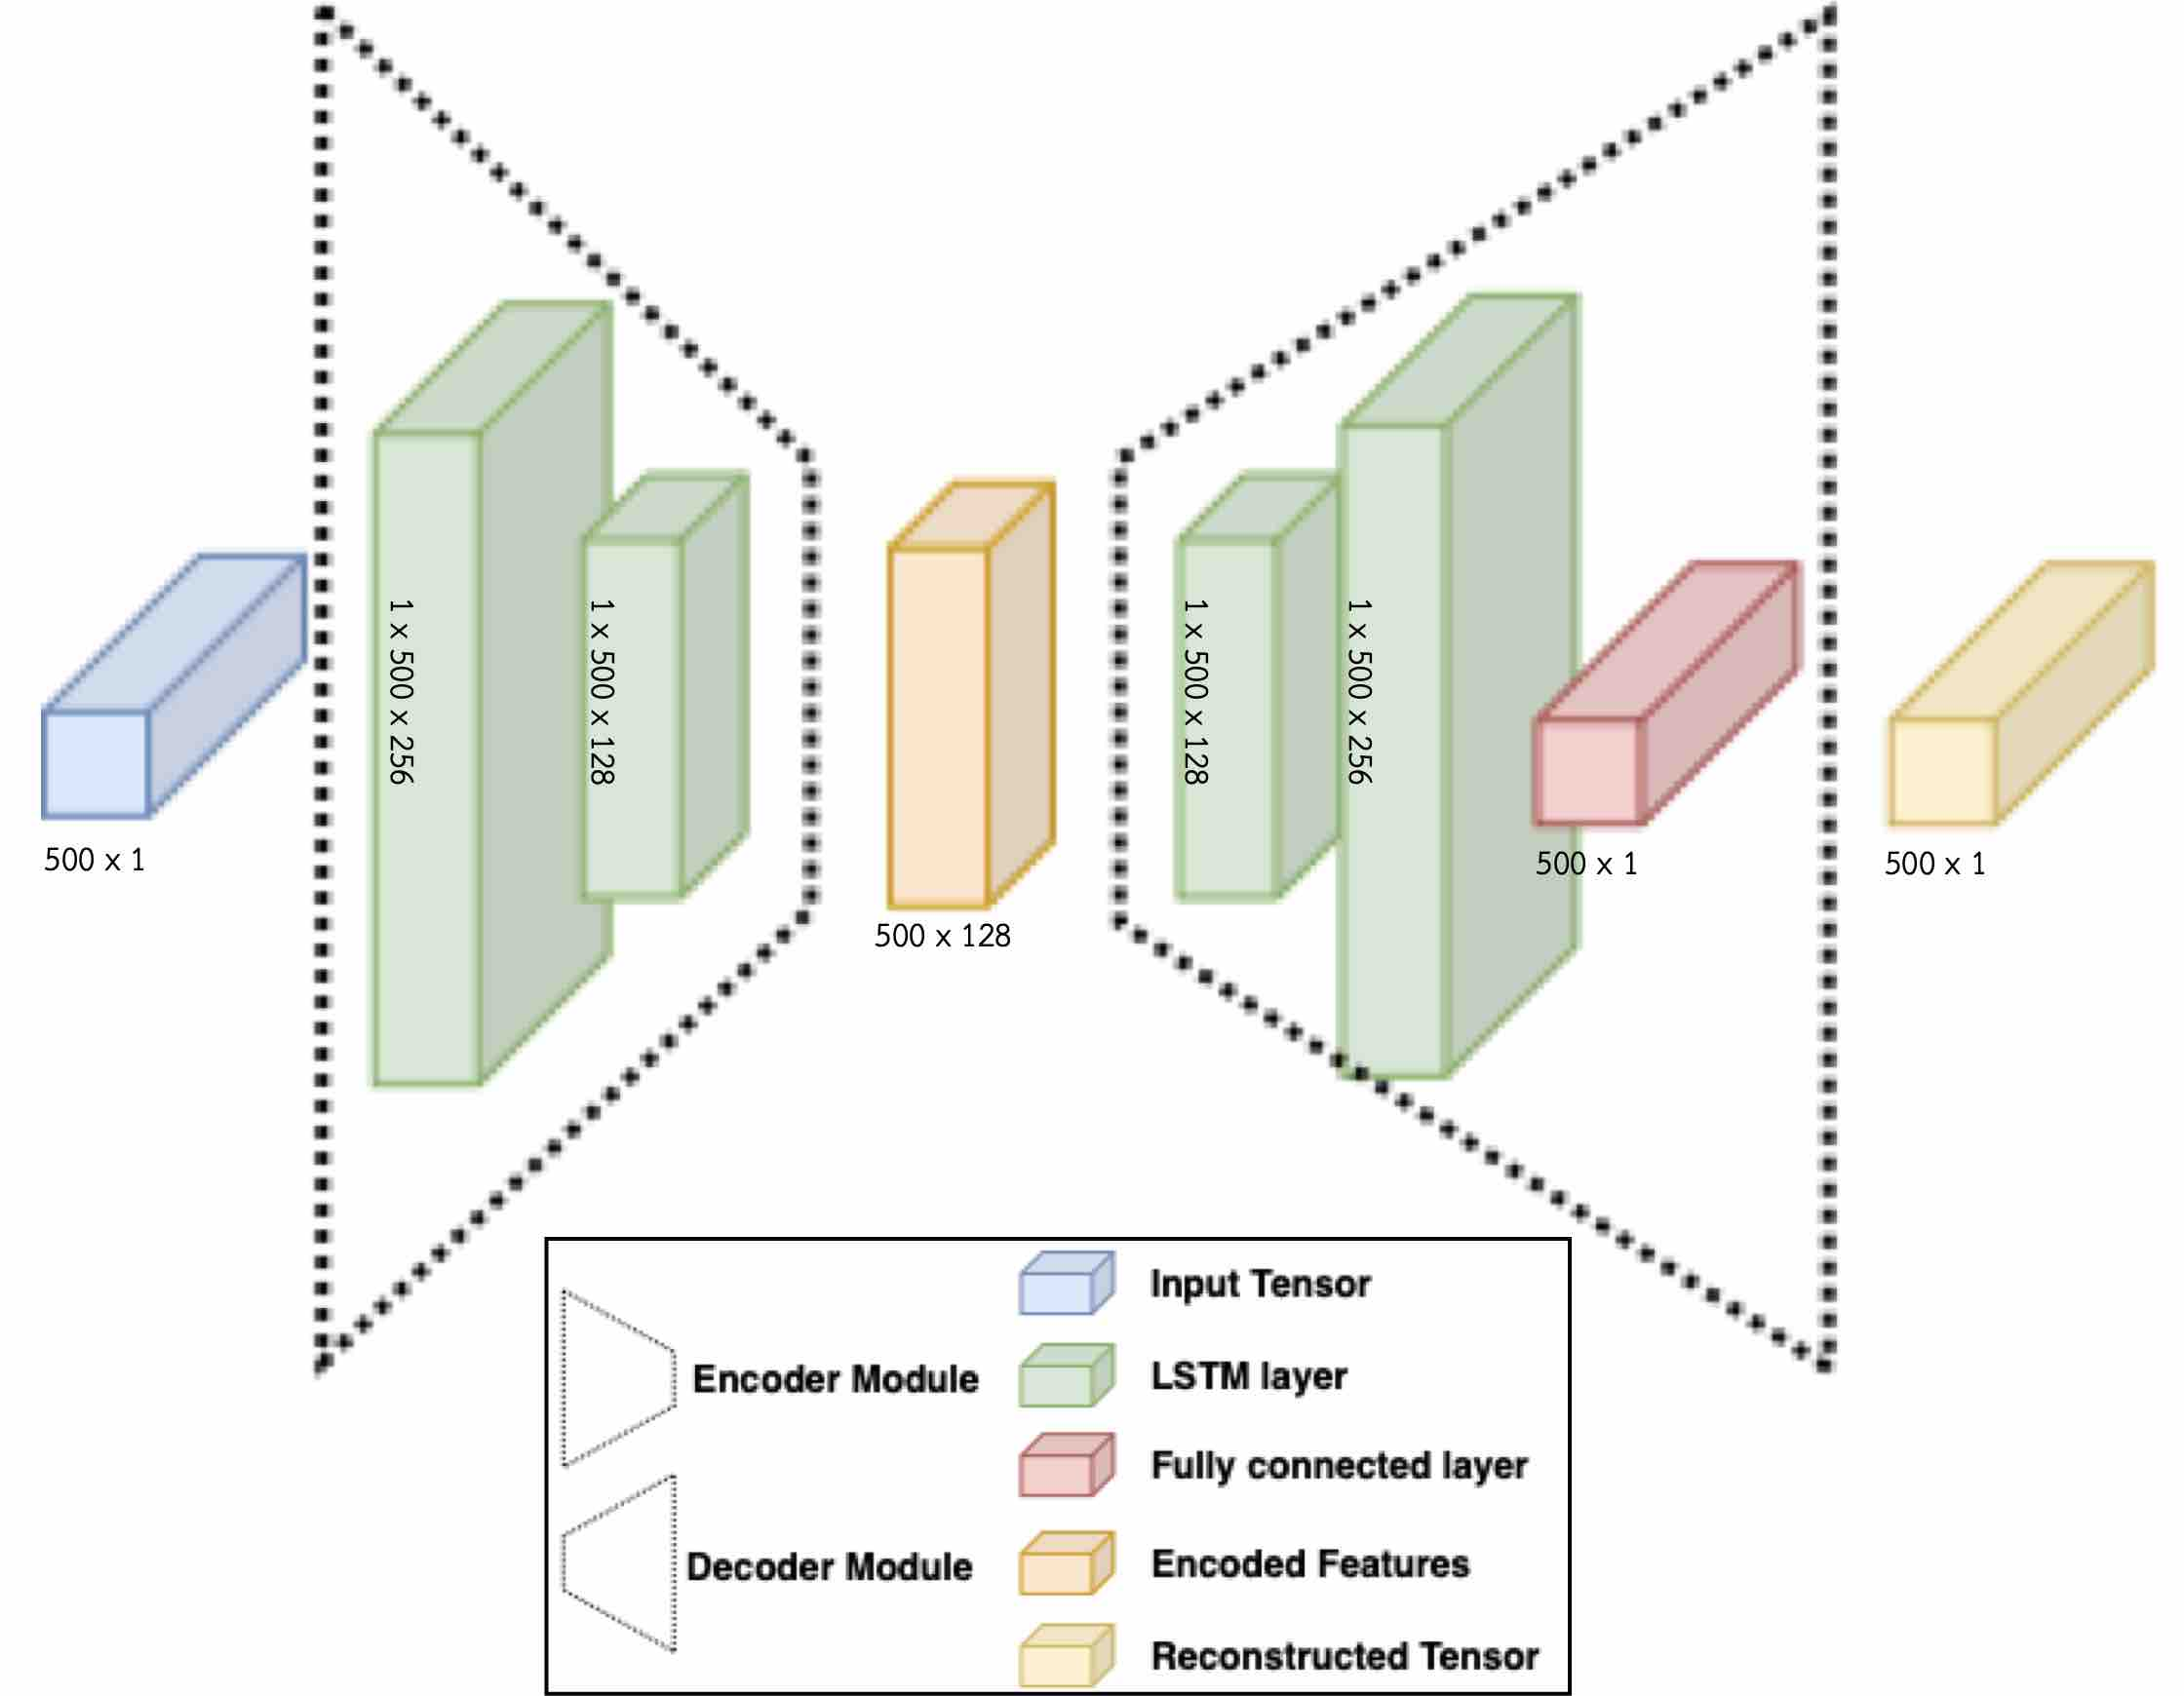
\includegraphics[scale = 0.22]{figures/autoencoder_lstm.jpg}
\end{figure}

\begin{figure}[H]
  \centering
  \caption[Convolutional anomaly detection autoencoder.]{\emph{Convolutional anomaly detection autoencoder.}} \label{fig:autoencoder_cnn}
  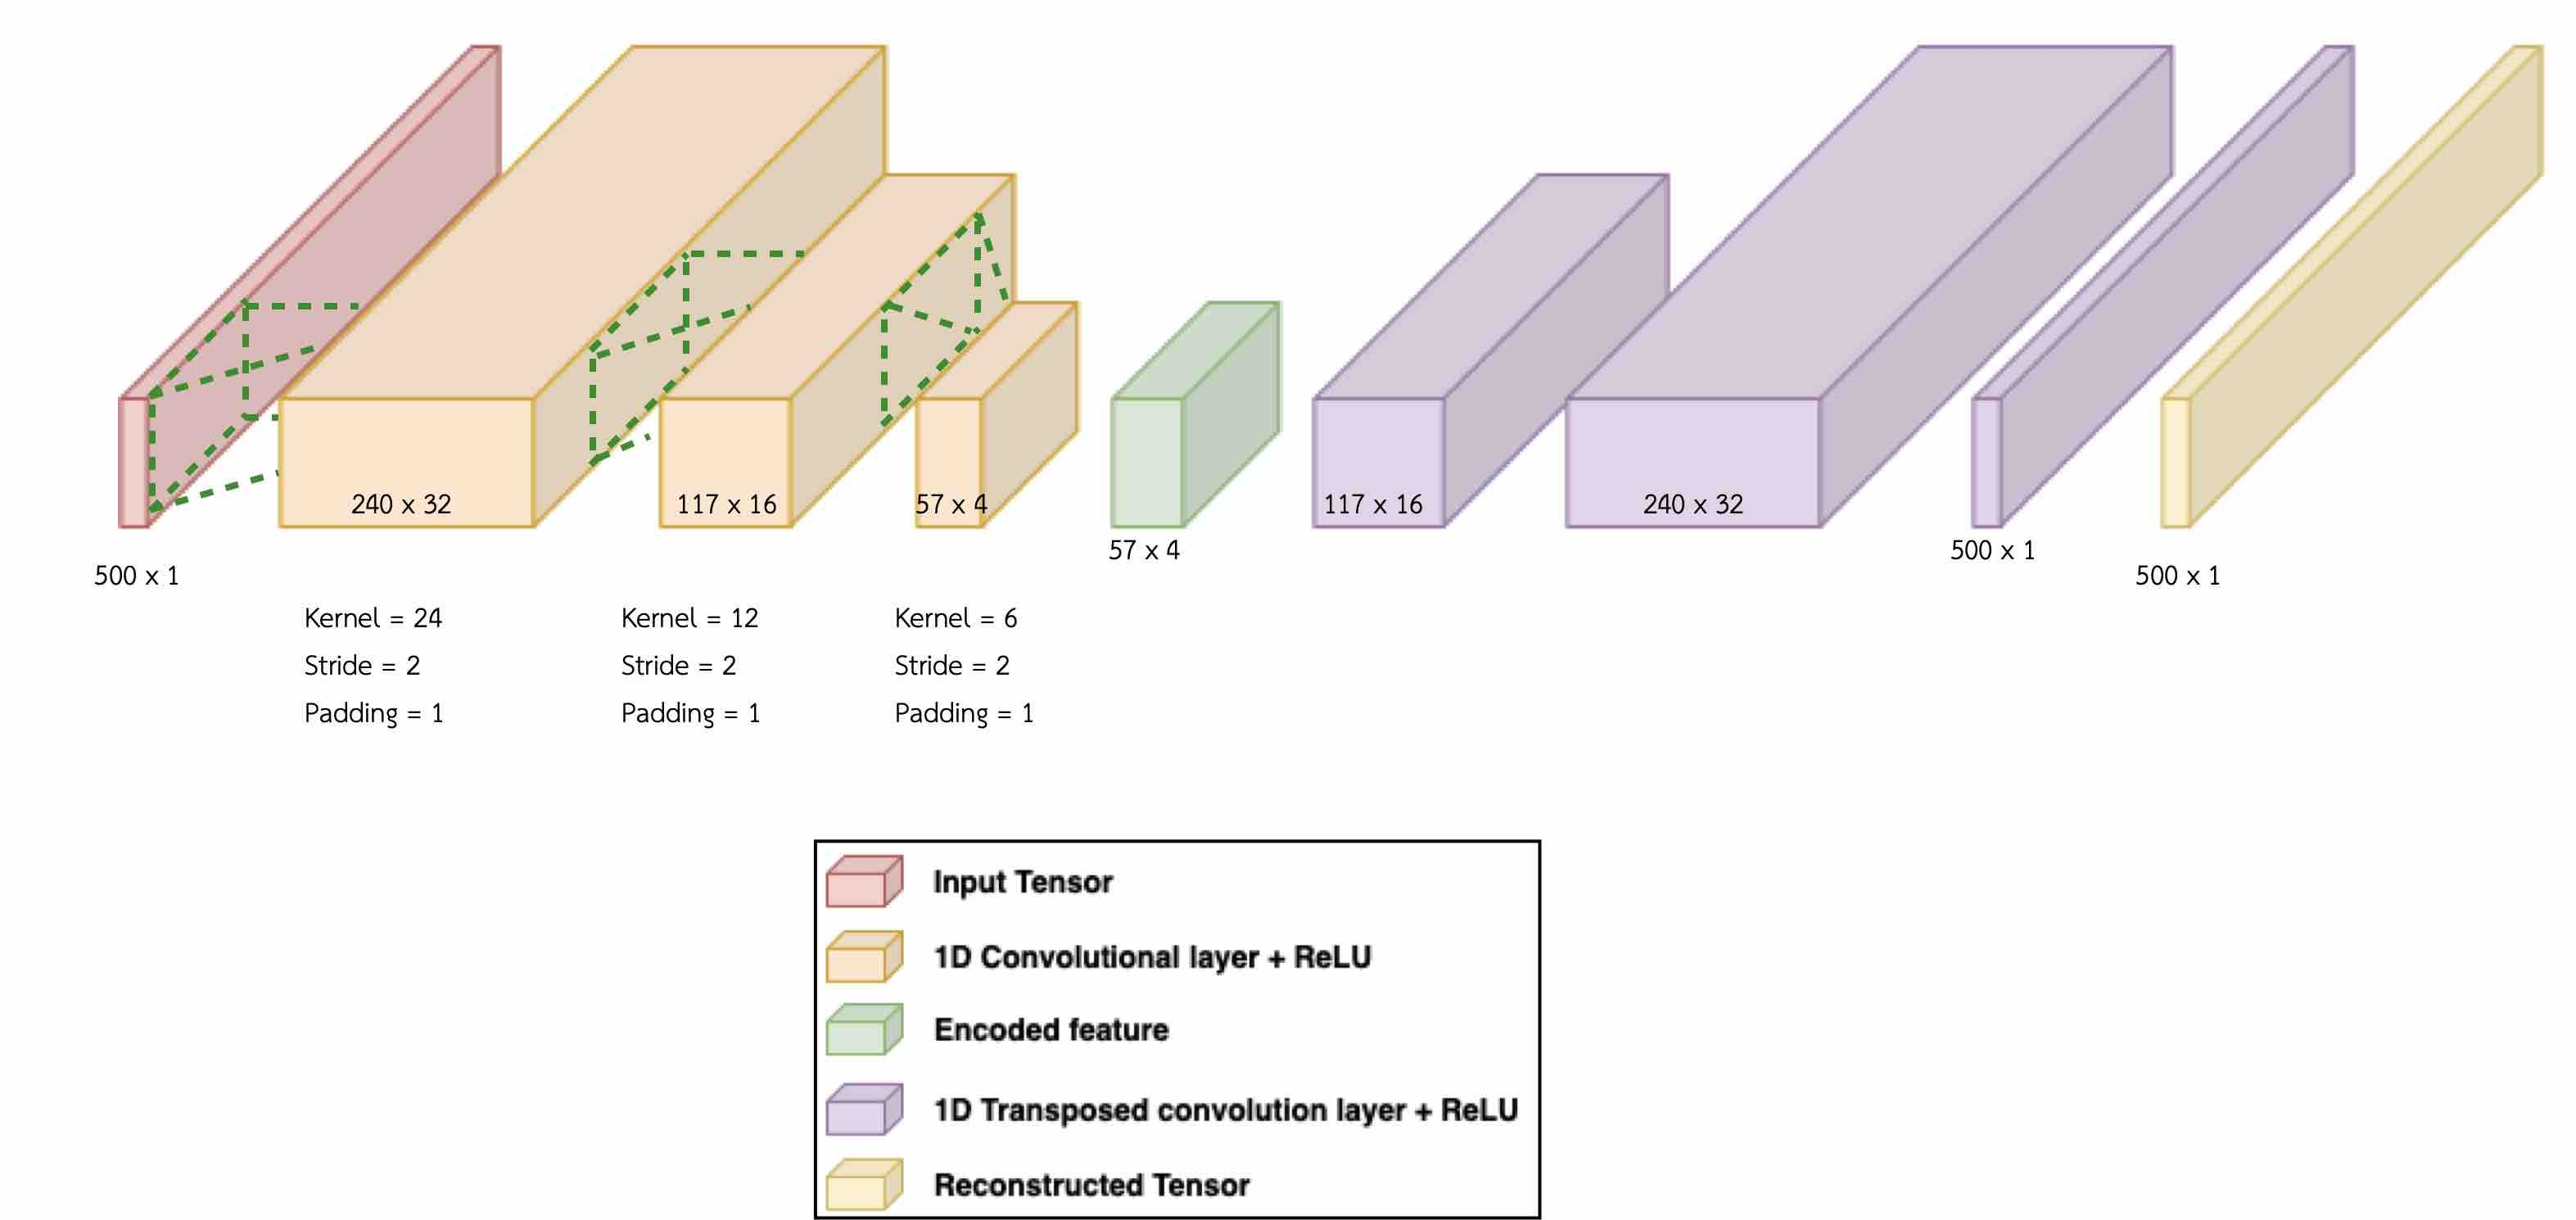
\includegraphics[scale = 0.15]{figures/autoencoder_cnn.jpg}
\end{figure}

\begin{figure}[H]
  \centering
  \caption[Convolutional + LSTM anomaly detection  autoencoder.]{\emph{Convolutional + LSTM anomaly detection  autoencoder.}} \label{fig:autoencoder_cnnlstm}
  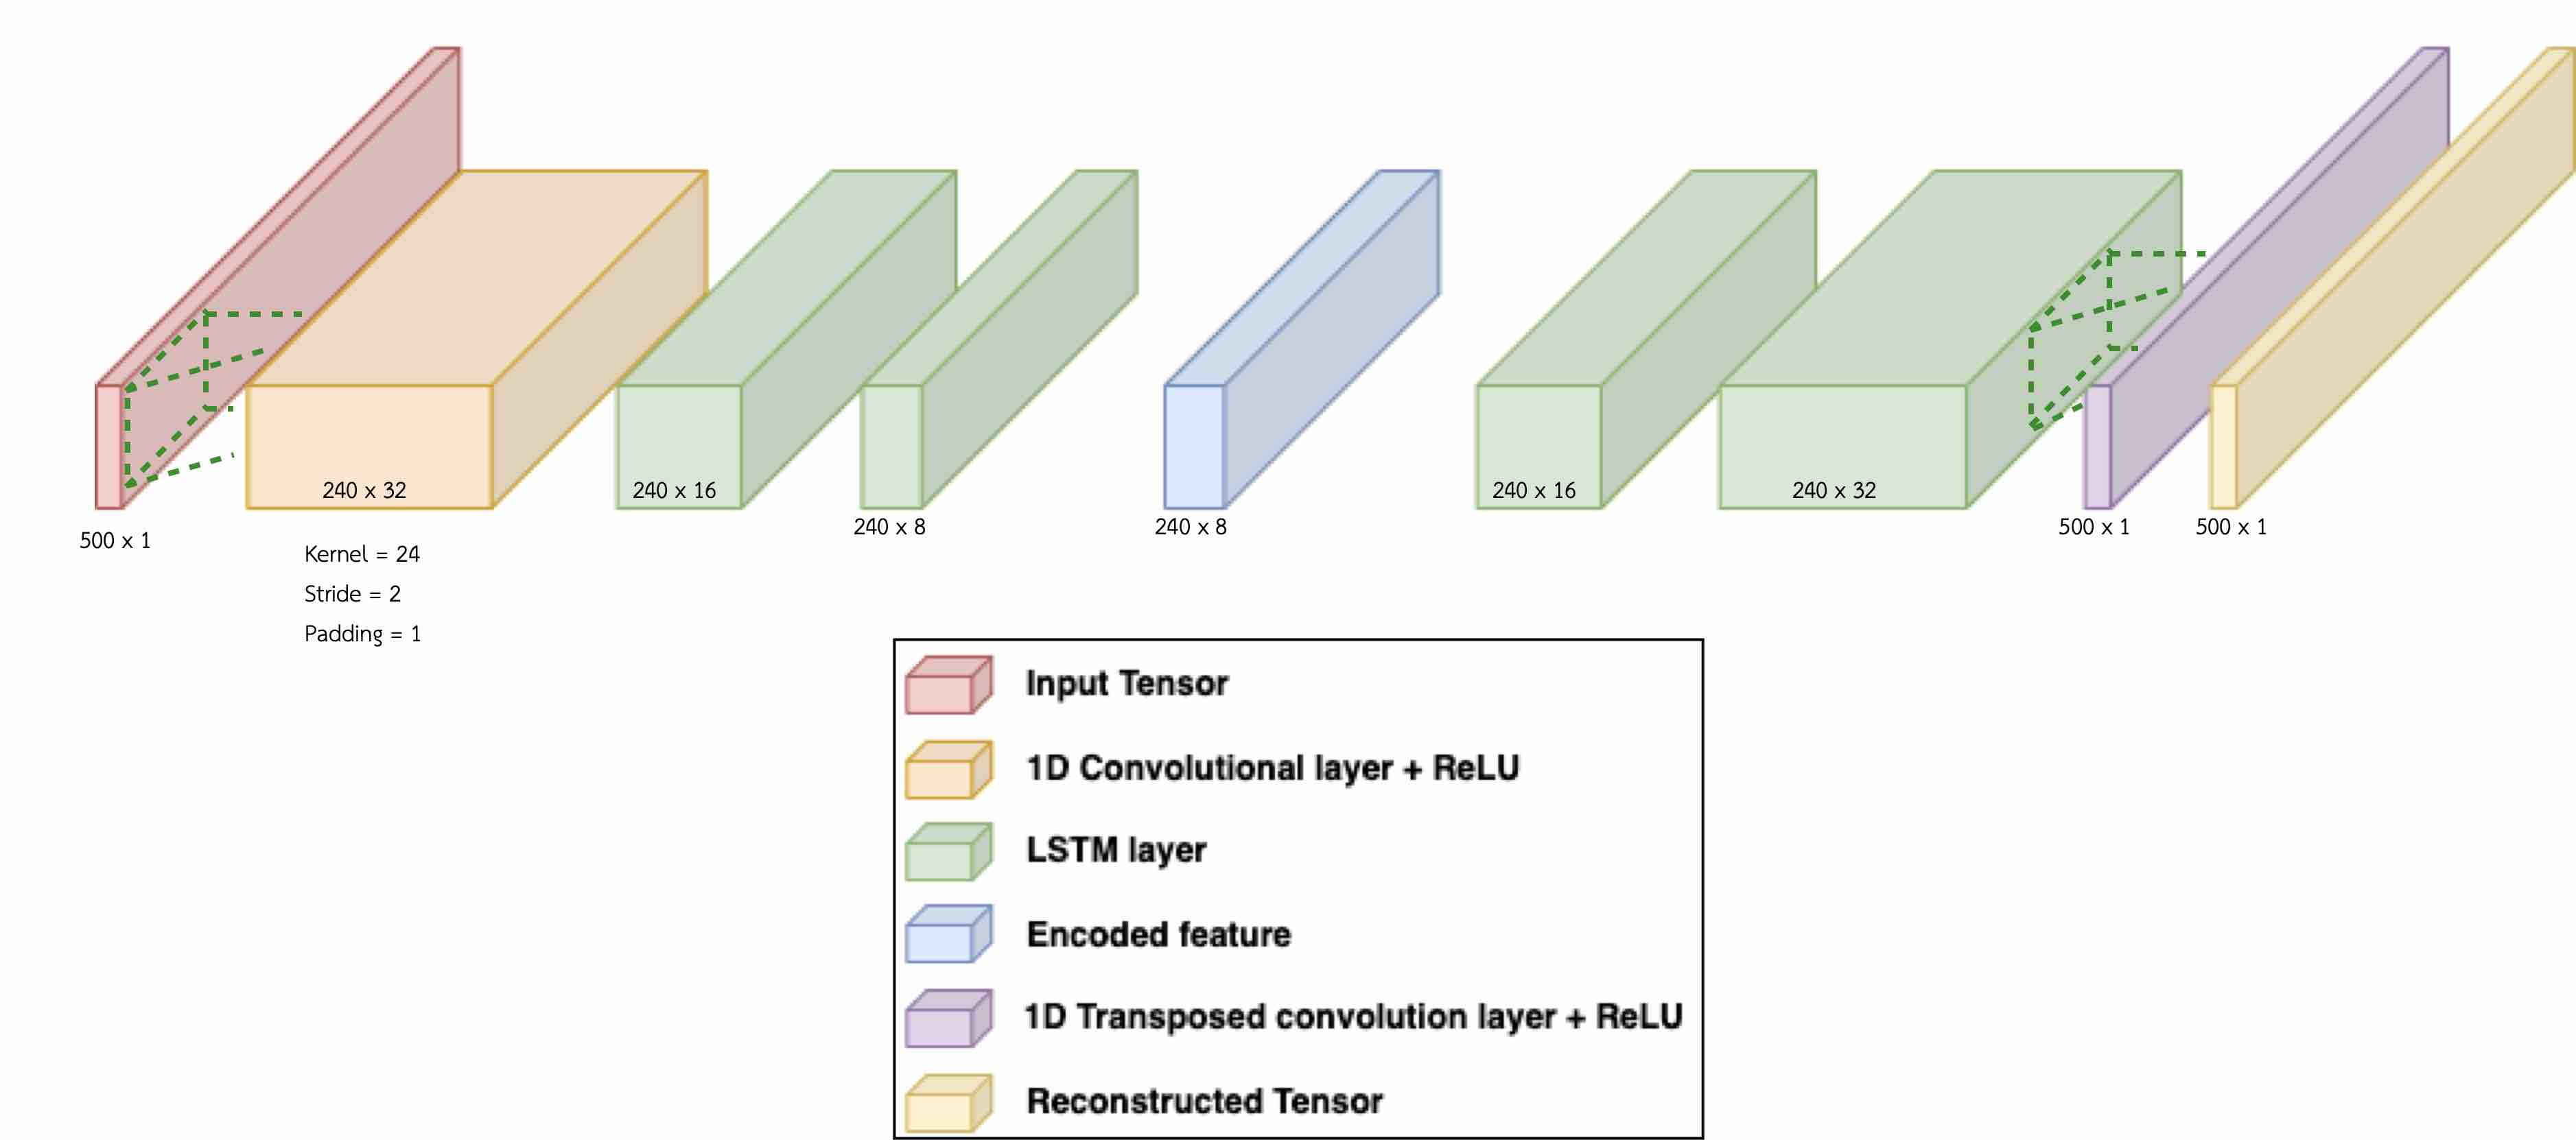
\includegraphics[scale = 0.13]{figures/autoencoder_cnnlstm.jpg}
\end{figure}

\begin{figure}[H]
  \centering
  \caption[Anomaly detection Transformer.]{\emph{Anomaly detection Transformer.}} \label{fig:transformer_1}
  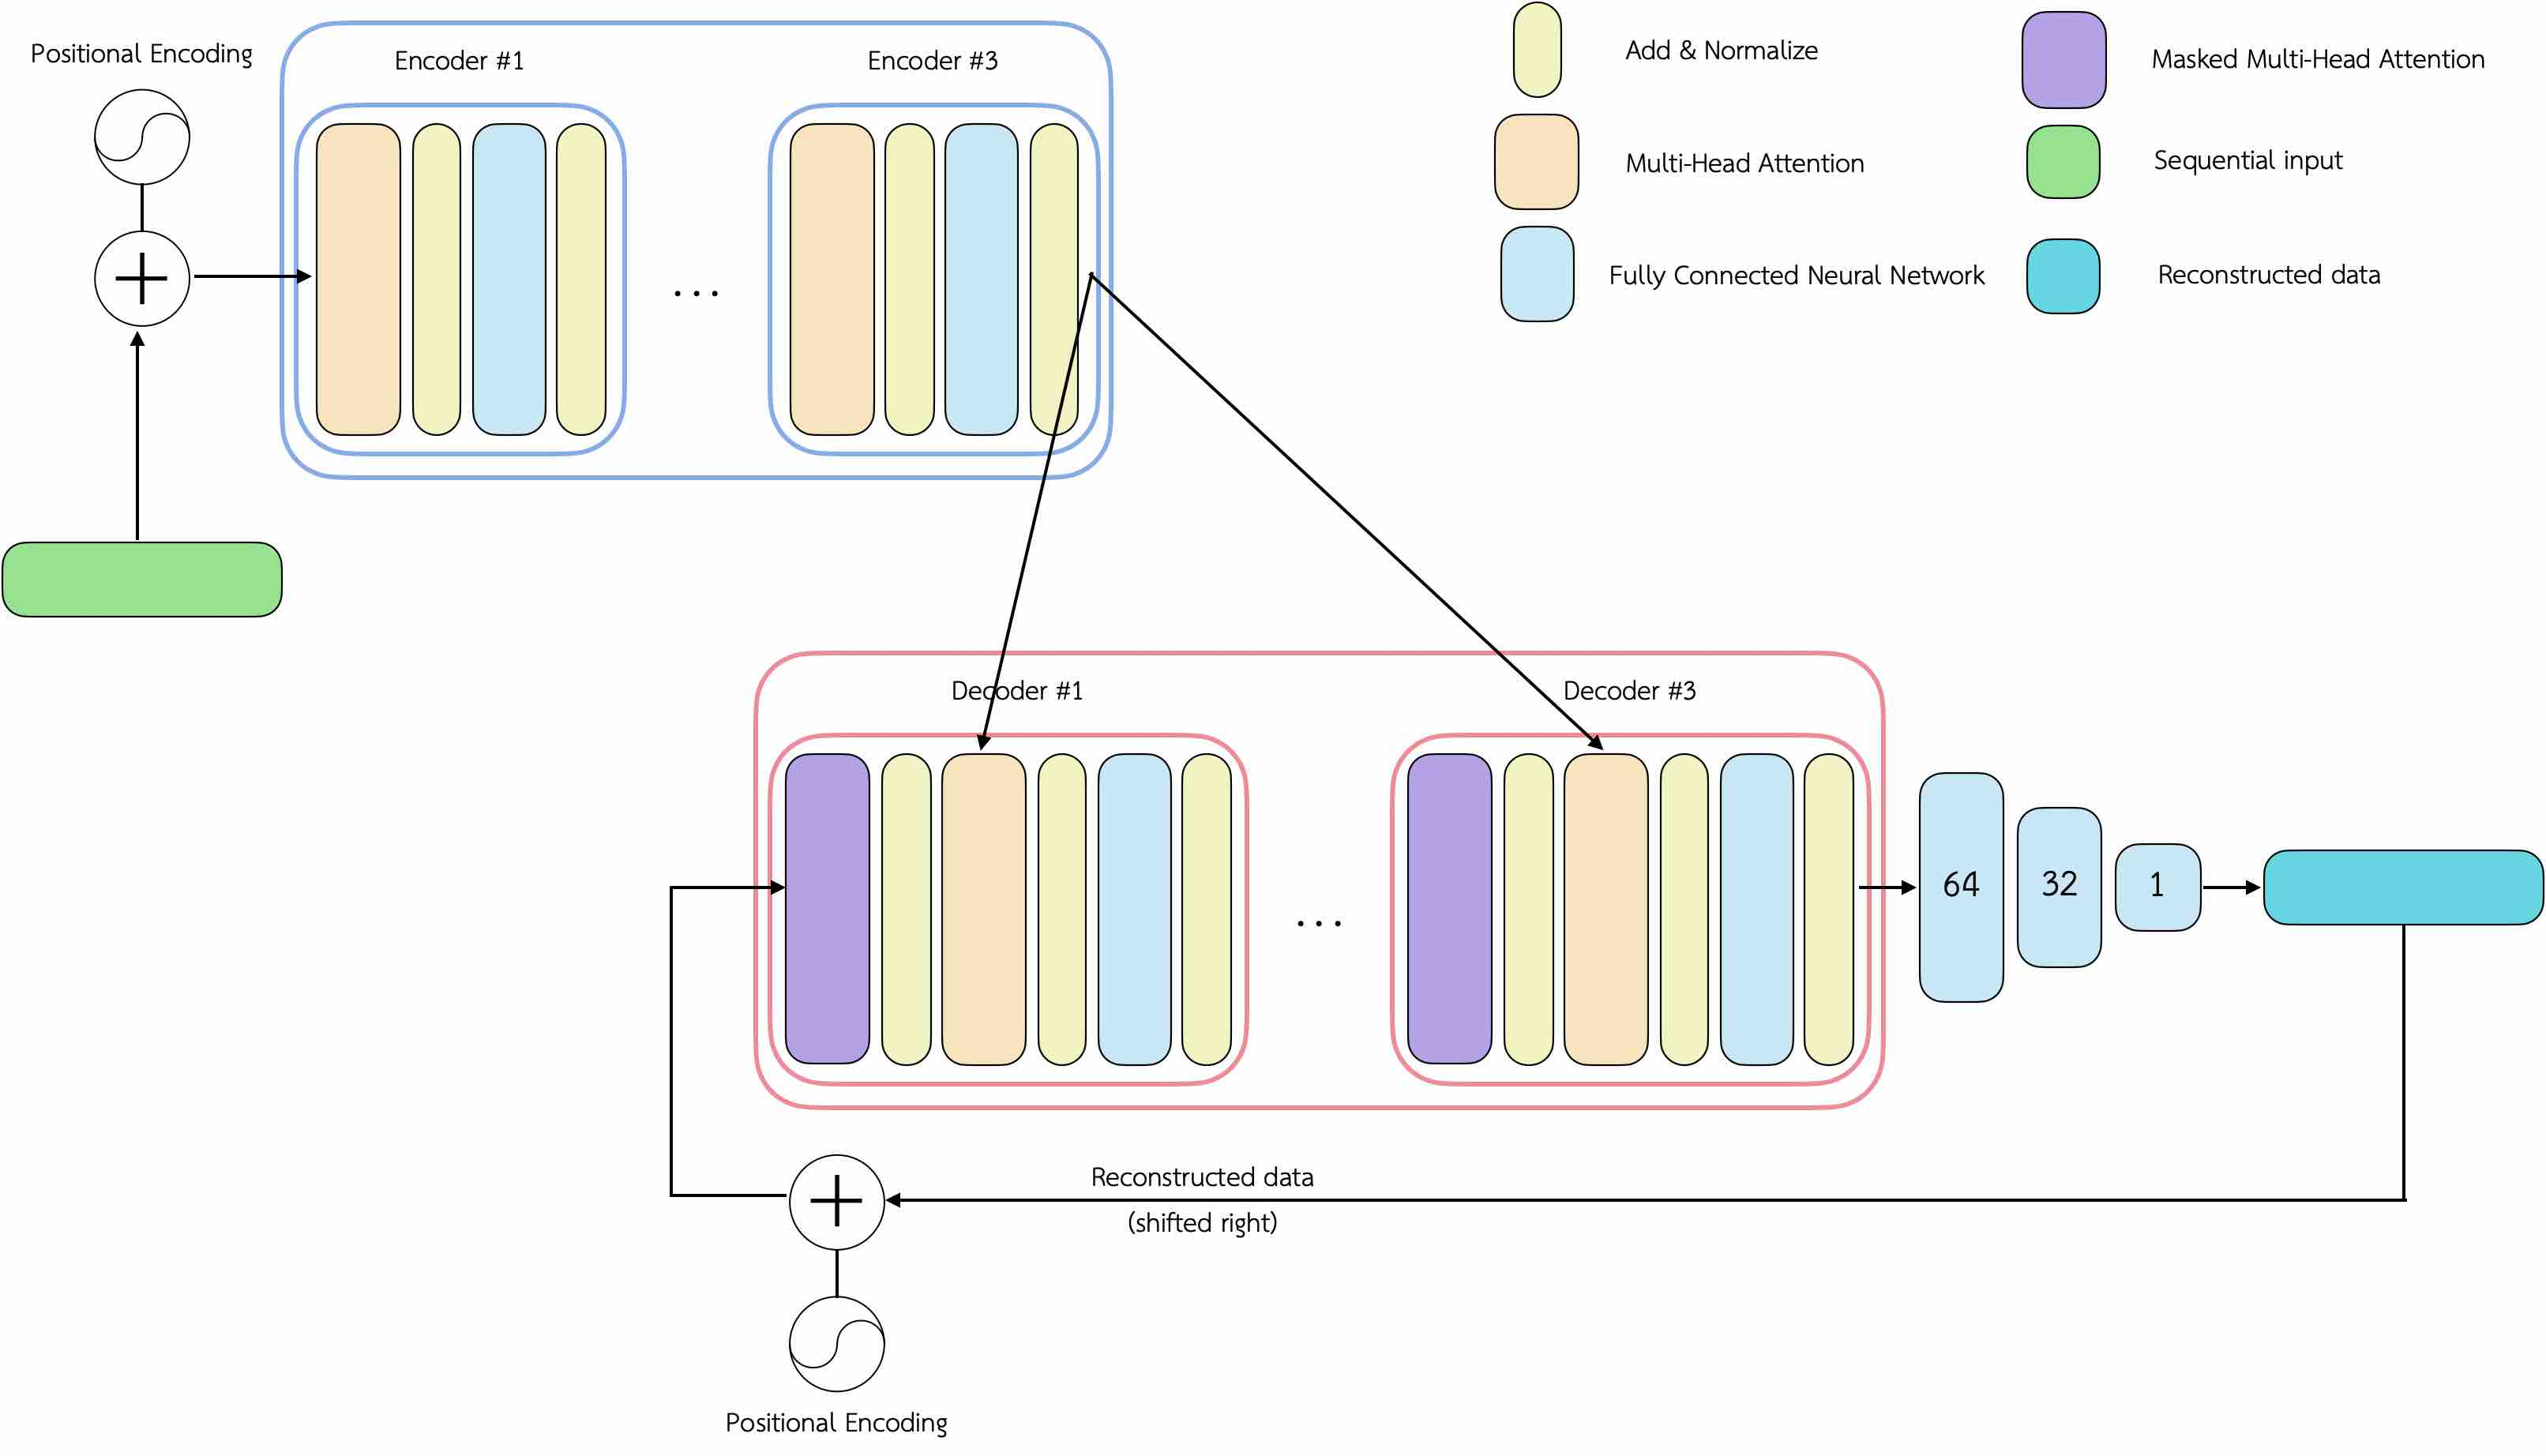
\includegraphics[scale = 0.15]{figures/transformer_job.jpg}
\end{figure}

\subsection{LSTM Autoencoder}
The encoder in the autoencoder with only LSTM (Figure \ref{fig:autoencoder_lstm}) uses two LSTM layers to compress the time series data input. The compressed representation is then decoded. The decoder also contains two LSTM layers in order to produce the final reconstructed data. Training takes approximately three minutes per epoch on a Intel Xeon E5-2620 v4 CPU @ 2.10GHz with a Geforce RTX 2080 GPU. Figure \ref{fig:autoencoder_outcome} shows the distribution of reconstruction error over the test set. The reconstruction error distributions for normal and abnormal activities are approximately normal with means of 19.60 and 64.10, respectively. With a threshold of 30.0, we obtain an accuracy of 89.08$\%$ for normal activities and 93.00$\%$ for anomalous activities, corresponding to 89.5$\%$ precision and F1 of 93.0$\%$ for the anomalous activities. Figure \ref{fig:autoencoder_reconstructed_data} compares the input signal and reconstructed data for normal and abnormal activities. Despite many attempts to adjust hyperparameter such as the learning rate, number of LSTM layers, and number of LSTM modules. The model had very poor reconstruction accuracy. Even though the autoencoder with LSTM architecture can separate the two classes perhaps based on amplitude alone, it clearly does not reconstruct well, apparently only regressing the mean.

\begin{figure}[H]
  \centering
  \caption[LSTM autoencoder reconstruction error distributions for normal and anomalous activities.]{\emph{LSTM autoencoder reconstruction error distributions for normal and anomalous activities.}} \label{fig:autoencoder_outcome}
  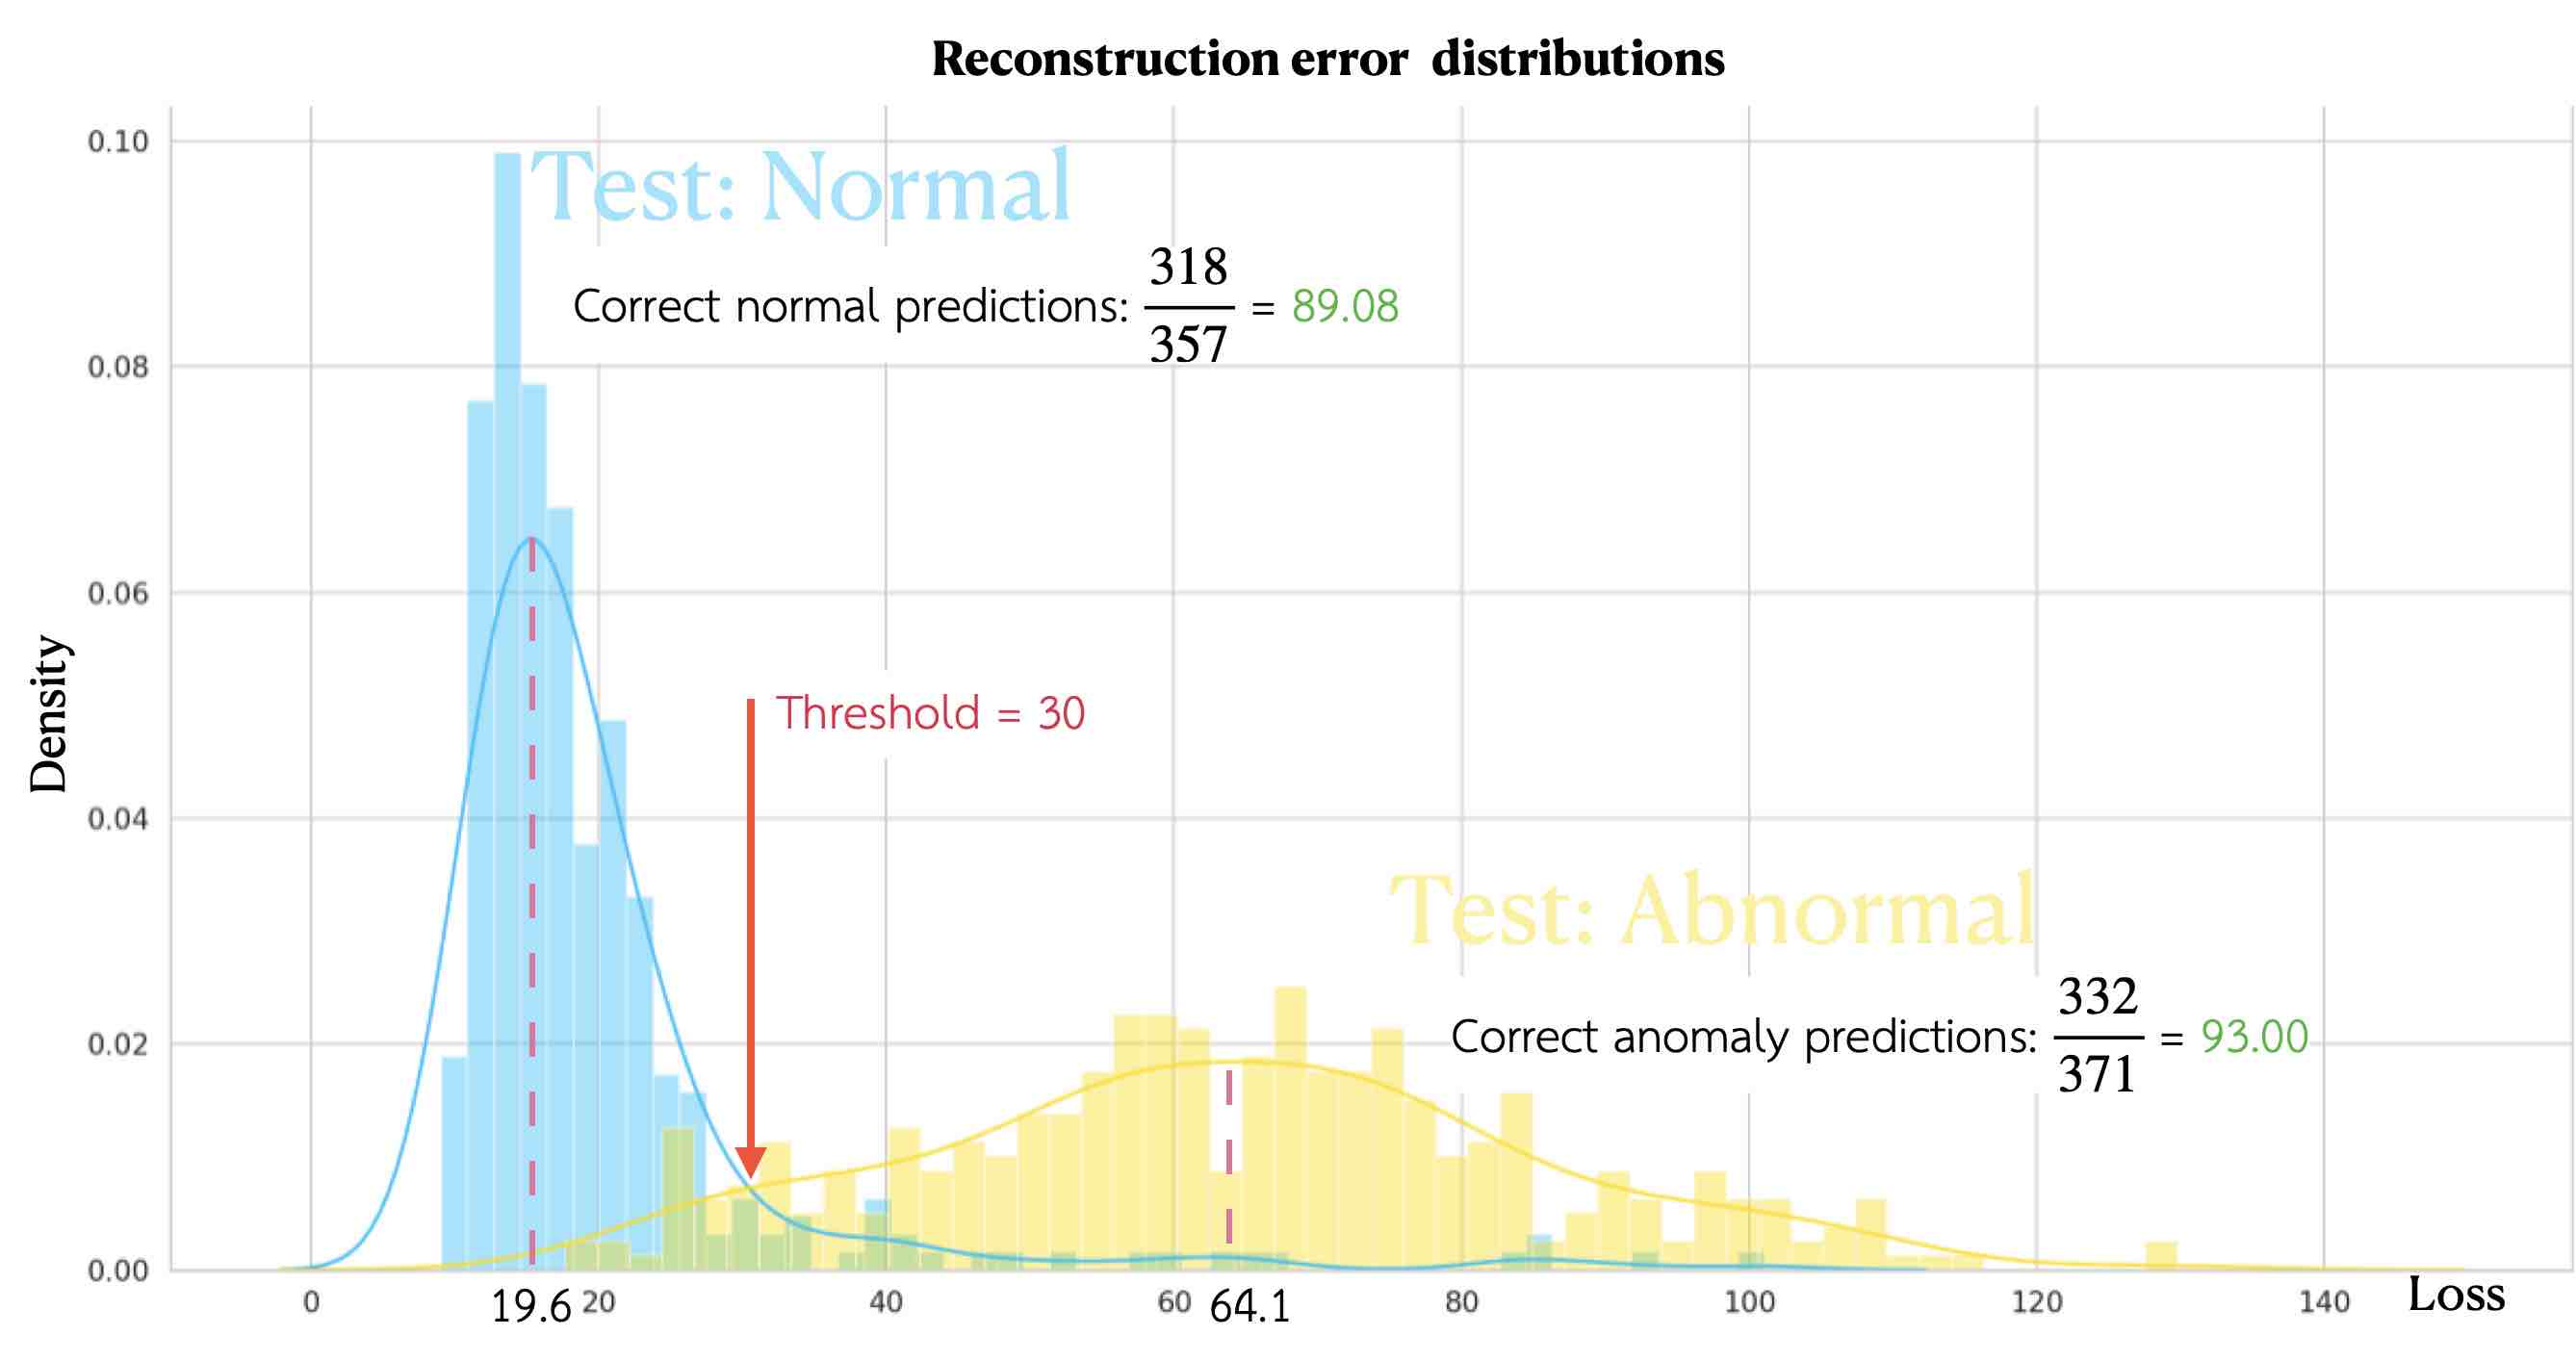
\includegraphics[scale = 0.18]{figures/autoencoder_outcome.jpg}
\end{figure}

\begin{figure}[H]
  \centering
  \caption[Reconstruction data of normal and abnormal activities using LSTM autoencoder.]{\emph{Reconstruction data of normal and abnormal activities using LSTM autoencoder.}} \label{fig:autoencoder_reconstructed_data}
  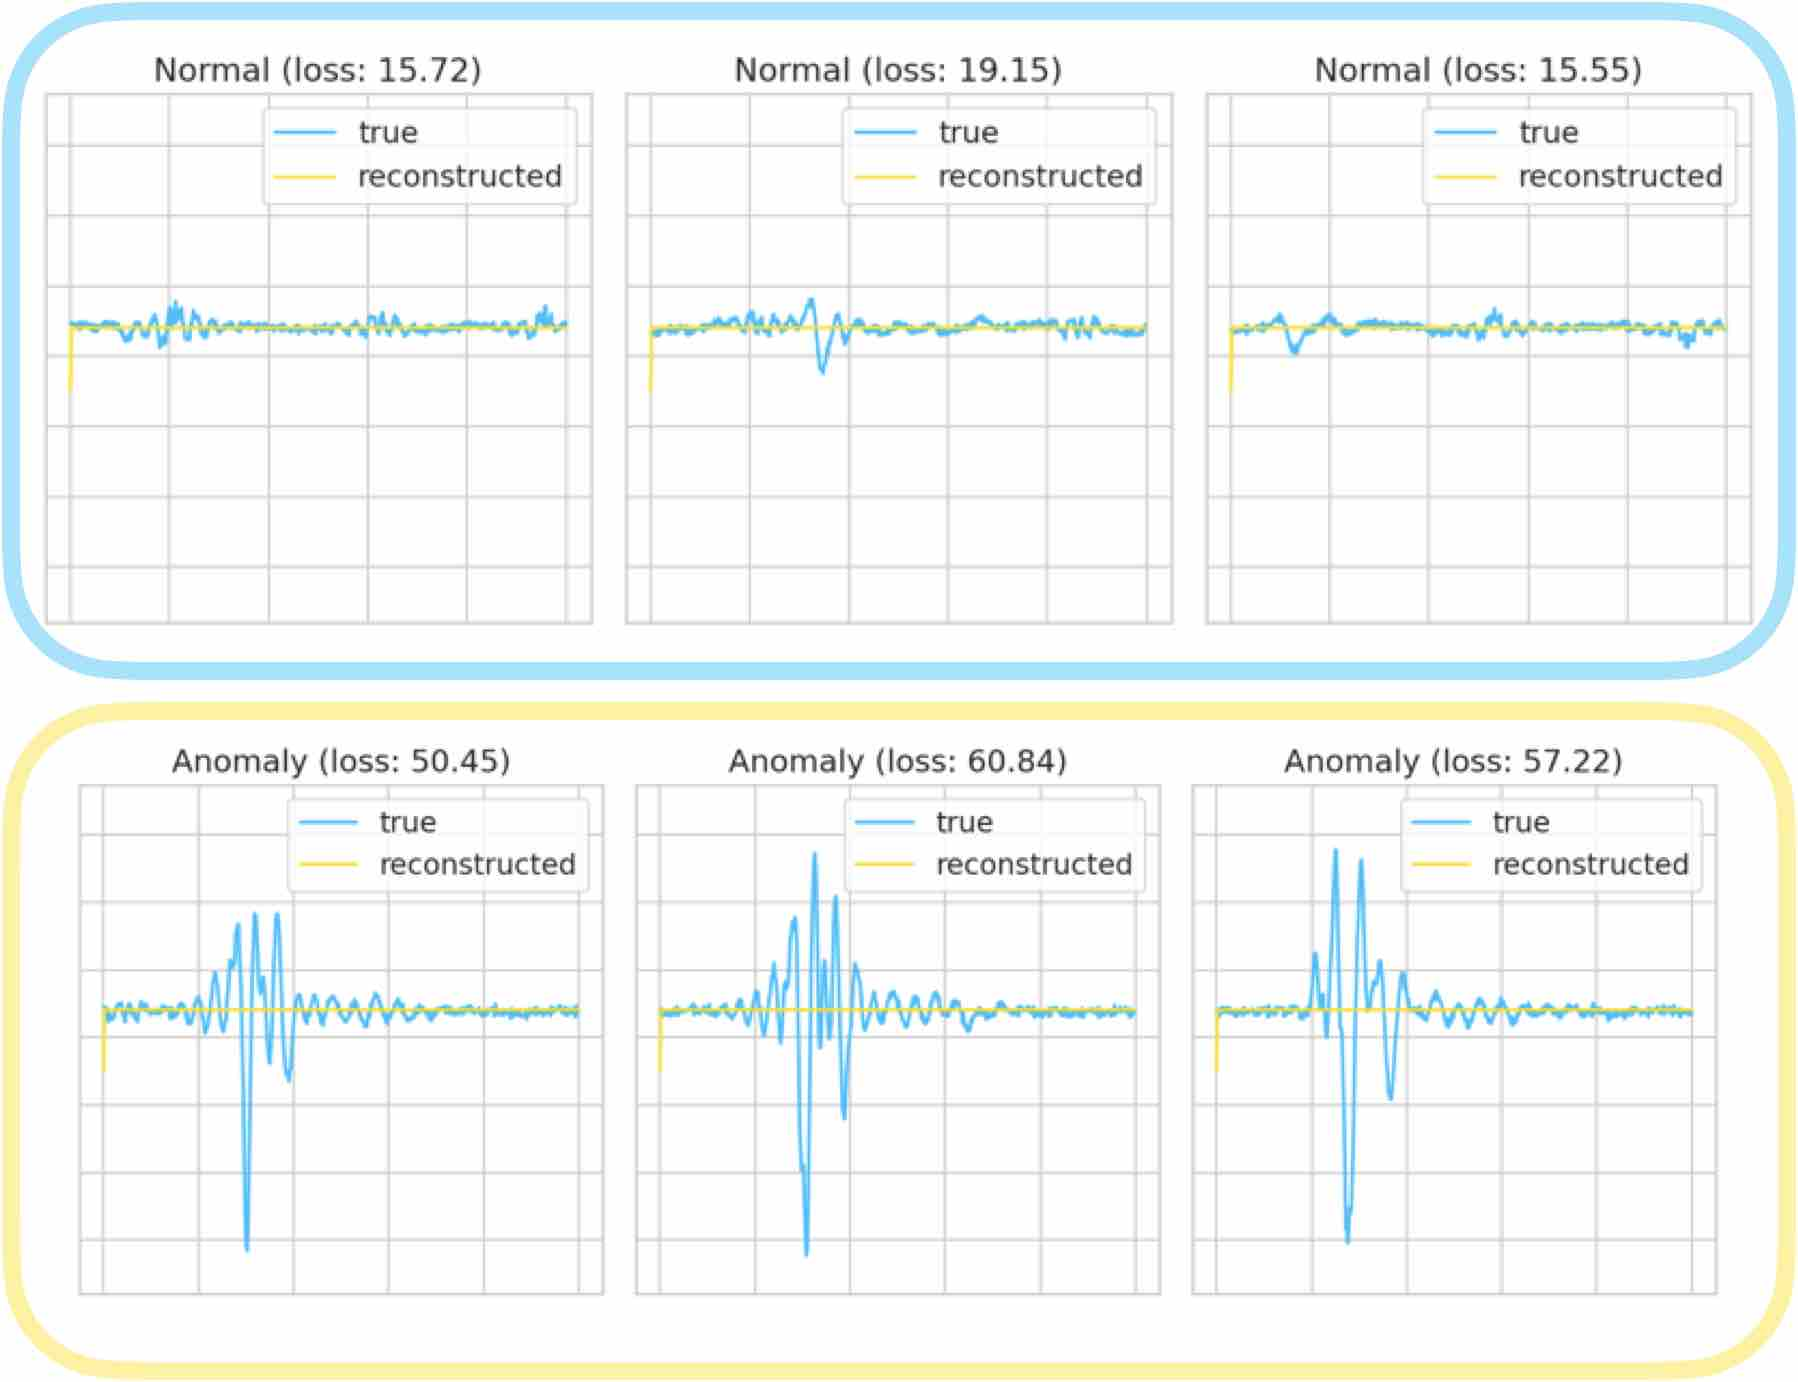
\includegraphics[scale = 0.2]{figures/autoencoder_reconstructed_data.jpg}
\end{figure}

\subsection{Convolutional Autoencoder}
The convolutional autoencoder is designed to be similar to the LSTM autoencoder, but we replace the LSTM layers wuth covolutional layer. Training takes approximately 13 seconds per epoch. The adjusted hyperparameters (number of output features and kernel size in each CNN layer) are shown in Table \ref{tab:cnn1t} and \ref{tab:cnn2t}. We select the best model according to F1 score from first trial to adjust kernel size in the second trial. Figure \ref{fig:autoencoder_cnn_outcome} shows the  distribution of reconstruction error over the test set. The reconstruction error distributions for normal and abnormal activities are approximately normal with means of 7.50 and 36.96, respectively. With a threshold of 13.0, we obtain an accuracy of 94.00$\%$ for normal activities and 92.72$\%$ for anomalous activities, giving 92.42$\%$ precision and 93.20$\%$ F1 score. Figure \ref{fig:autoencoder_cnn_reconstructed_data} compares the input signal and reconstructed data for normal and abnormal activities. It seems that the convolutional layers can help the model reconstructed the input more effectively than the LSTM autoencoder.

\begin{table}[H]
  \begin{center}
    \caption[First trial: adjust number of output feature of convolutional layers.]{\emph{First trial: adjust number of output feature of convolutional layers.} \\ \hspace{\textwidth}}\label{tab:cnn1t}
    \begin{tabular}{c c c c c c c}
      \hline
      \multicolumn{2}{c}{\multirow{2}{*}{\textbf{Output feature}}} & \multicolumn{4}{c}{\textbf{Accuracy (\%)}} & \multirow{2}{*}{\textbf{Threshold}}                                      \\
      \cline{3-6}
                                                                   &                                            & Normal events                       & Abnormal events & Precision & F1 & \\
      \hline
      \multicolumn{2}{l}{64 -$>$ 32 -$>$ 16 : 32 -$>$ 64 -$>$ 1}   & 93.94                                      & 83.03                               & 84.07           & 89.08     & 13   \\
      \multicolumn{2}{l}{32 -$>$ 16 -$>$  8 : 16 -$>$ 32 -$>$ 1}   & 94.00                                      & 92.72                               & 92.42           & 93.20     & 13   \\
      \multicolumn{2}{l}{16 -$>$  8 -$>$  4 :  8 -$>$ 16 -$>$ 1}   & 88.48                                      & 90.30                               & 90.12           & 89.30     & 10   \\
      \hline
    \end{tabular}
  \end{center}
\end{table}

\begin{table}[H]
  \begin{center}
    \caption[Second trial: adjust kernel size of in convolutional layers.]{\emph{Second trial: adjust kernel size of in convolutional layers.} \\ \hspace{\textwidth}}\label{tab:cnn2t}
    \begin{tabular}{c c c c c c c}
      \hline
      \multicolumn{2}{c}{\multirow{2}{*}{\textbf{Kernel size}}}   & \multicolumn{4}{c}{\textbf{Accuracy (\%)}} & \multirow{2}{*}{\textbf{Threshold}}                                      \\
      \cline{3-6}
                                                                  &                                            & Normal events                       & Abnormal events & Precision & F1 & \\
      \hline
      \multicolumn{2}{c}{12 -$>$  6 -$>$  3 :  3 -$>$  6 -$>$ 12} & 89.09                                      & 86.67                               & 86.98           & 88.02     & 6    \\
      \multicolumn{2}{c}{24 -$>$ 12 -$>$  6 :  6 -$>$ 12 -$>$ 24} & 94.00                                      & 92.72                               & 92.42           & 93.20     & 13   \\
      \multicolumn{2}{c}{64 -$>$ 32 -$>$ 16 : 16 -$>$ 32 -$>$ 64} & 88.48                                      & 90.30                               & 90.12           & 89.30     & 15   \\
      \hline
    \end{tabular}
  \end{center}
\end{table}

\begin{figure}[H]
  \centering
  \caption[1DCNN autoencoder reconstruction error distributions for normal and anomalous activities.]{\emph{1DCNN autoencoder reconstruction error distributions for normal and anomalous activities.}} \label{fig:autoencoder_cnn_outcome}
  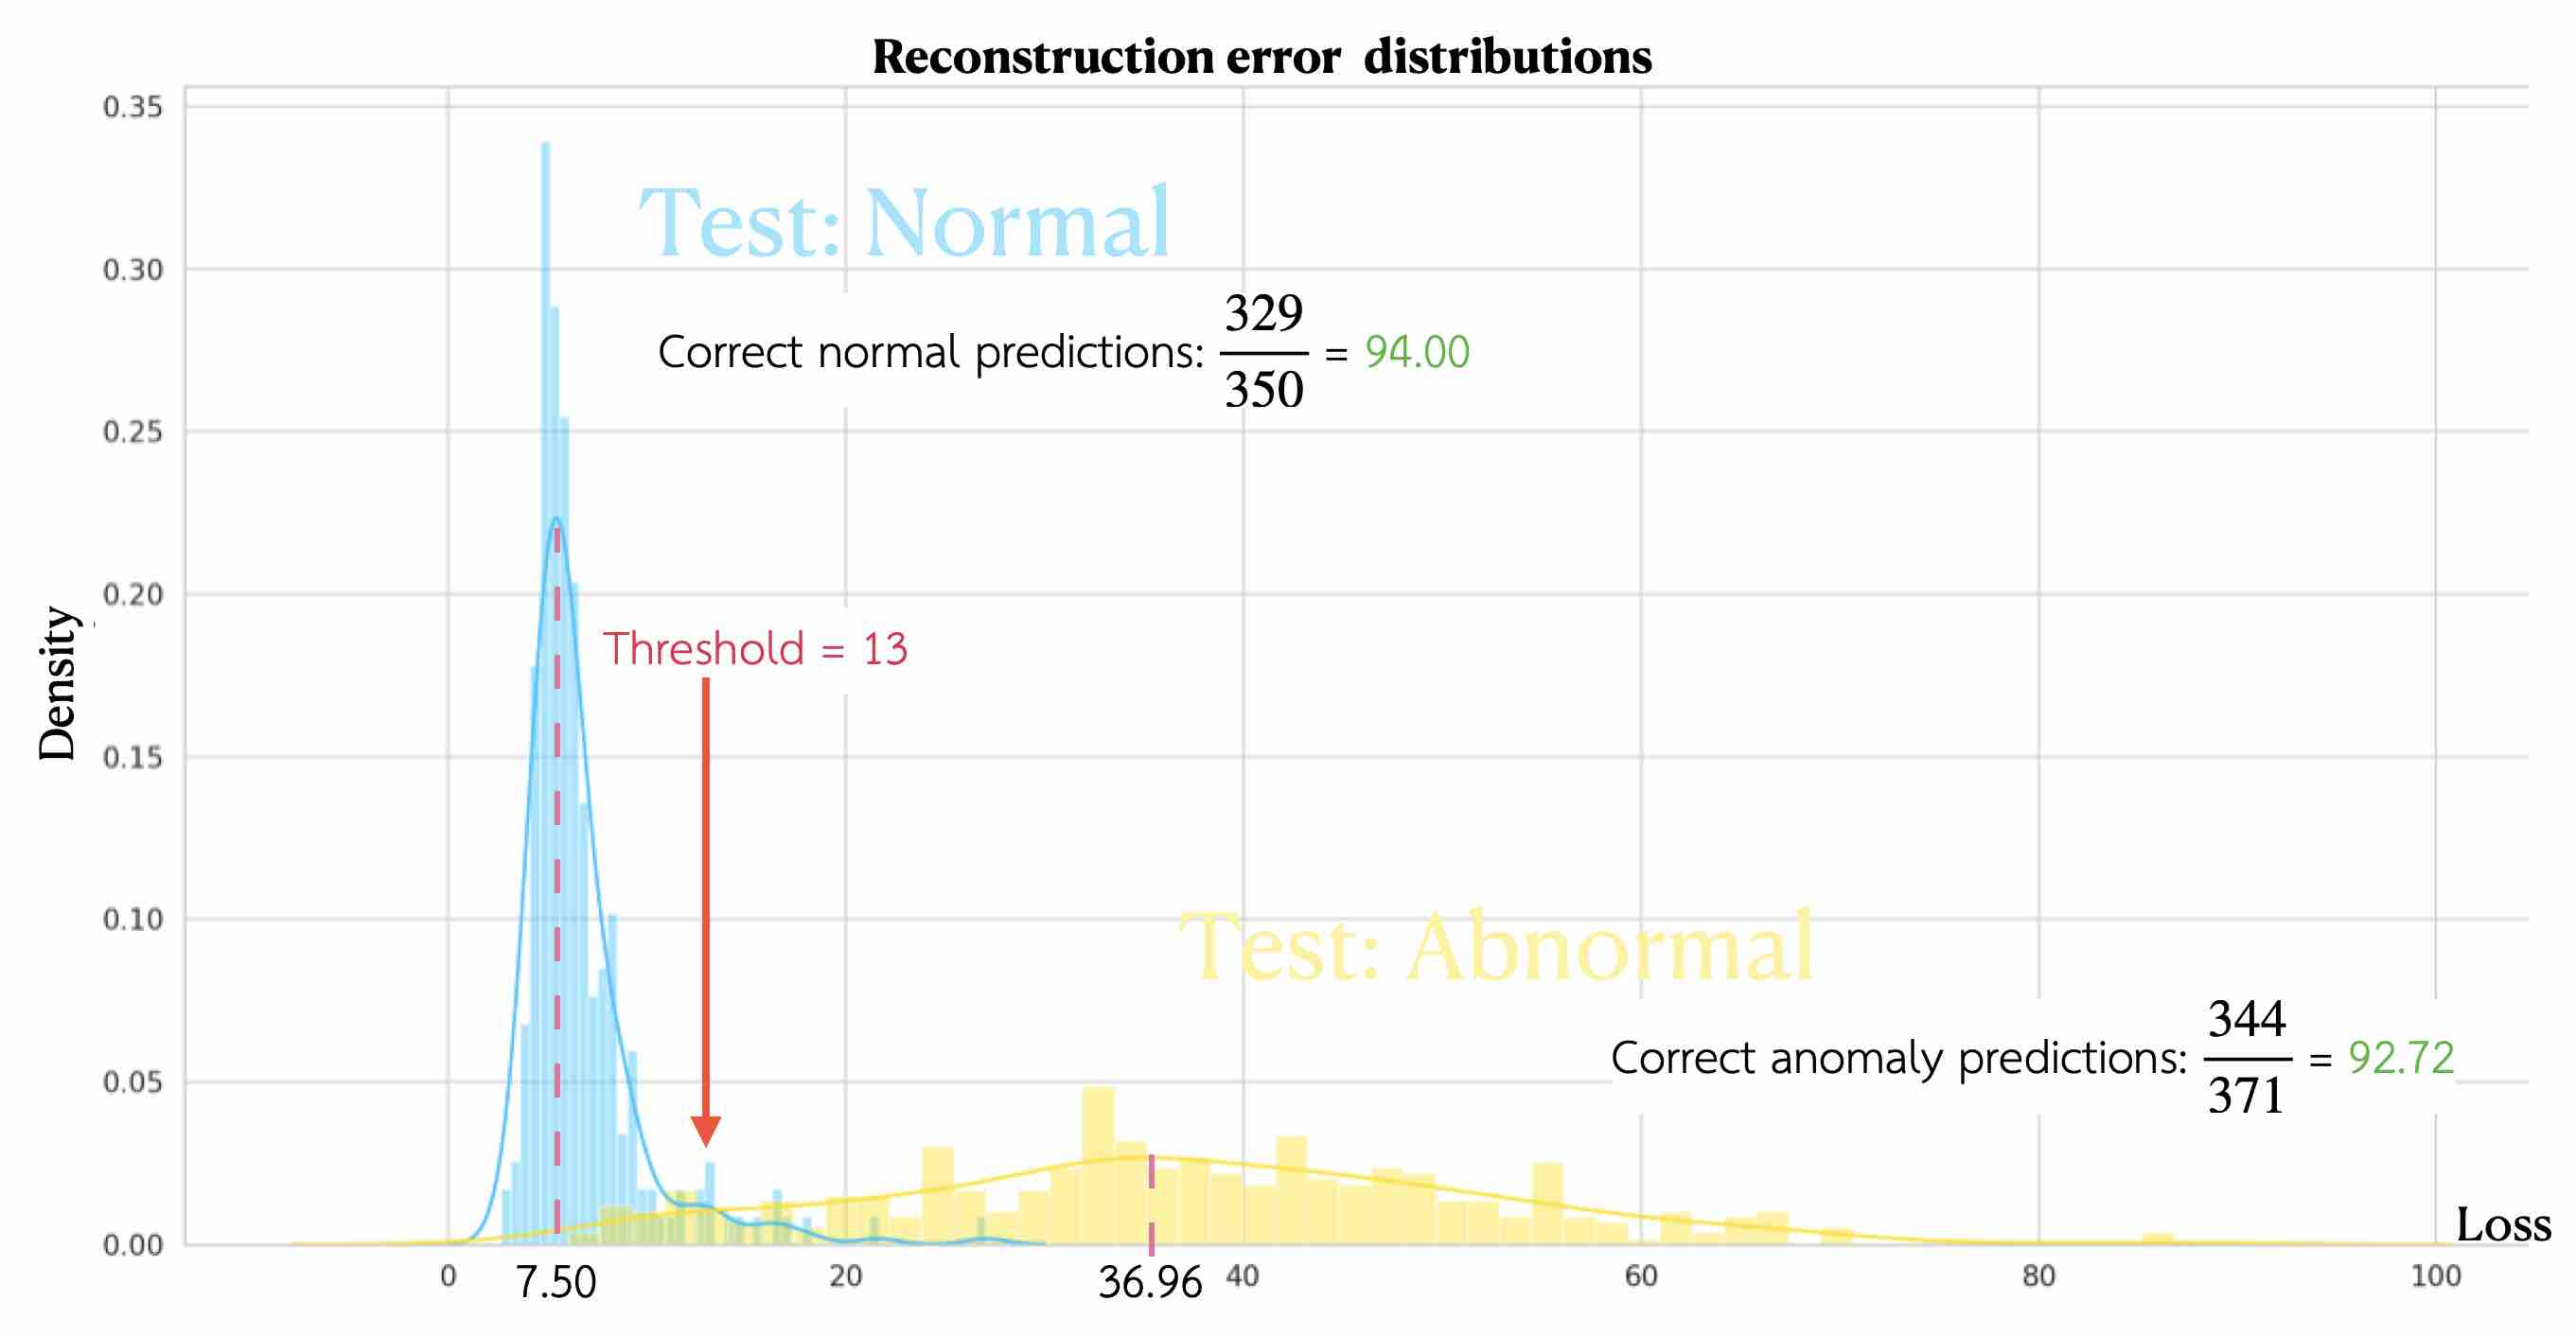
\includegraphics[scale = 0.18]{figures/autoencoder_cnn_outcome.jpg}
\end{figure}

\begin{figure}[H]
  \centering
  \caption[Reconstruction of normal and abnormal activities using 1DCNN autoencoder.]{\emph{Reconstruction of normal and abnormal activities using 1DCNN autoencoder.}} \label{fig:autoencoder_cnn_reconstructed_data}
  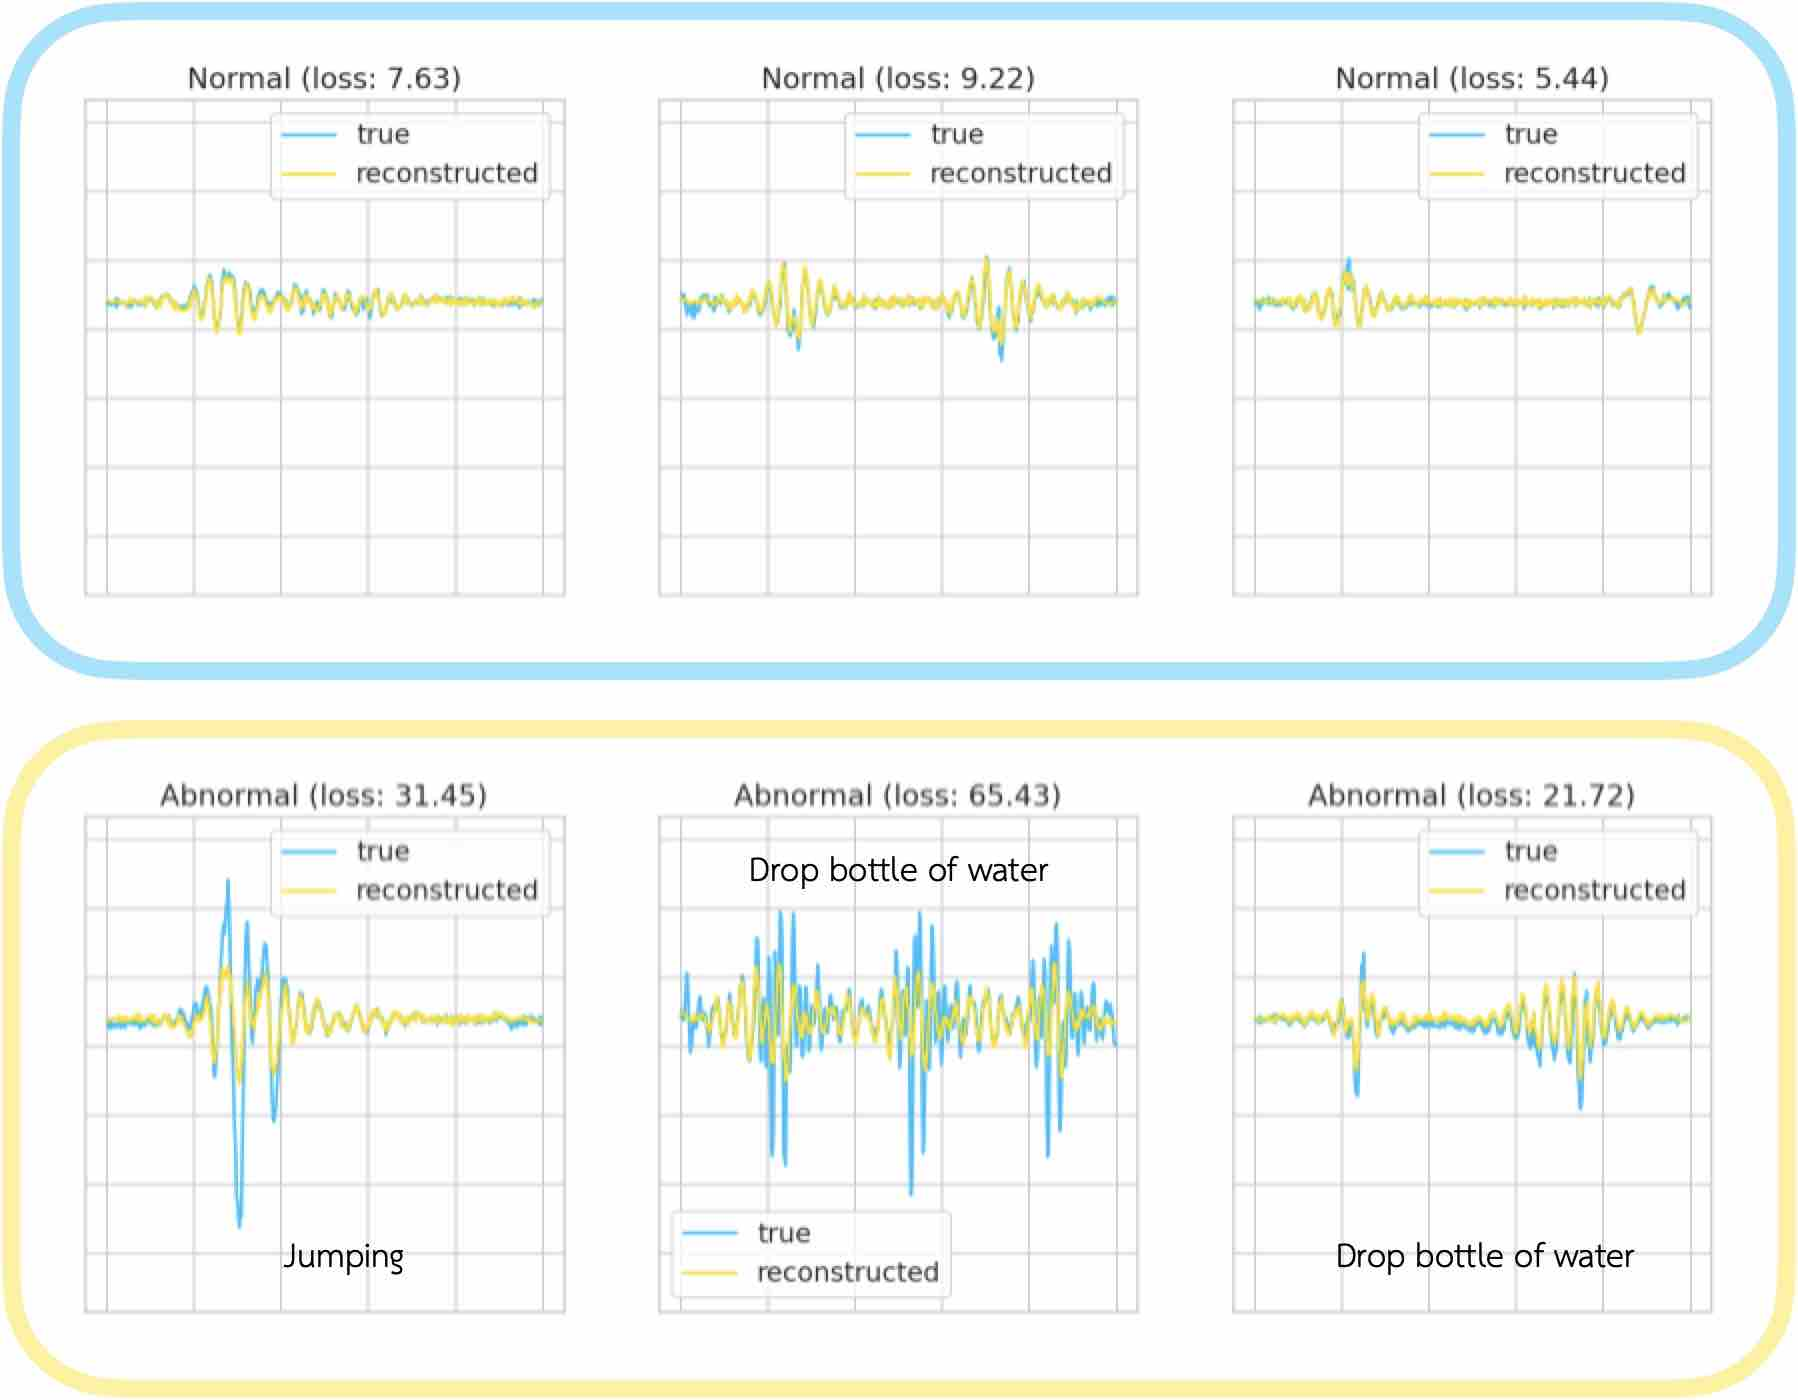
\includegraphics[scale = 0.22]{figures/autoencoder_cnn_reconstructed_data.jpg}
\end{figure}

\subsection{CNN + LSTM Autoencoder}
Here we combine the CNN and LSTM to get a CNN + LSTM autoencoder. Training takes approximately 95 seconds per epoch. We copy the configuration of CNN from the previous model and adjust only the output features of the LSTM layer. The configuration is shown in Table \ref{tab:cnnlstm}. Figure \ref{fig:autoencoder_cnnlstm_outcome} shows the distribution of reconstruction error over the test set. The reconstruction error distributions for normal and abnormal activities are approximately normal with means of 4.55 and 40.00, respectively. With a threshold of 10.0, we obtain an accuracy of 93.71$\%$ for normal activities and 93.26$\%$ for anomalous activities, giving a 92.92$\%$ precision and 93.31$\%$ F1 score. Reconstructions by the CNN + LSTM autoencoder are shown in Figure \ref{fig:autoencoder_cnnlstm_reconstructed_data}.


\begin{table}[H]
  \begin{center}
    \caption[Adjusting number of output feature in LSTM layer.]{\emph{Adjusting number of output feature in LSTM layer.} \\ \hspace{\textwidth}}\label{tab:cnnlstm}
    \begin{tabular}{c c c c c c c}
      \hline
      \multicolumn{2}{c}{\multirow{2}{*}{\textbf{Output feature}}} & \multicolumn{4}{c}{\textbf{Accuracy (\%)}} & \multirow{2}{*}{\textbf{Threshold}}                                      \\
      \cline{3-6}
                                                                   &                                            & Normal events                       & Abnormal events & Precision & F1 & \\
      \hline
      \multicolumn{2}{c}{ 4 -$>$  2:  4 -$>$  32}                  & 94.57                                      & 87.87                               & 88.03           & 91.18     & 17   \\
      \multicolumn{2}{c}{ 8 -$>$  4:  8 -$>$  32}                  & 92.29                                      & 92.29                               & 92.55           & 92.53     & 9    \\
      \multicolumn{2}{c}{16 -$>$  8:  8 -$>$  32}                  & 93.71                                      & 93.26                               & 92.92           & 93.31     & 10   \\
      \multicolumn{2}{c}{32 -$>$ 16: 32 -$>$  32}                  & 96.57                                      & 98.65                               & 98.38           & 92.10     & 7    \\
      \hline
    \end{tabular}
  \end{center}
\end{table}

\begin{figure}[H]
  \centering
  \caption[1DCNN + LSTM autoencoder reconstruction error distributions for normal and anomalous activities.]{\emph{1DCNN + LSTM autoencoder reconstruction error distributions for normal and anomalous activities.}} \label{fig:autoencoder_cnnlstm_outcome}
  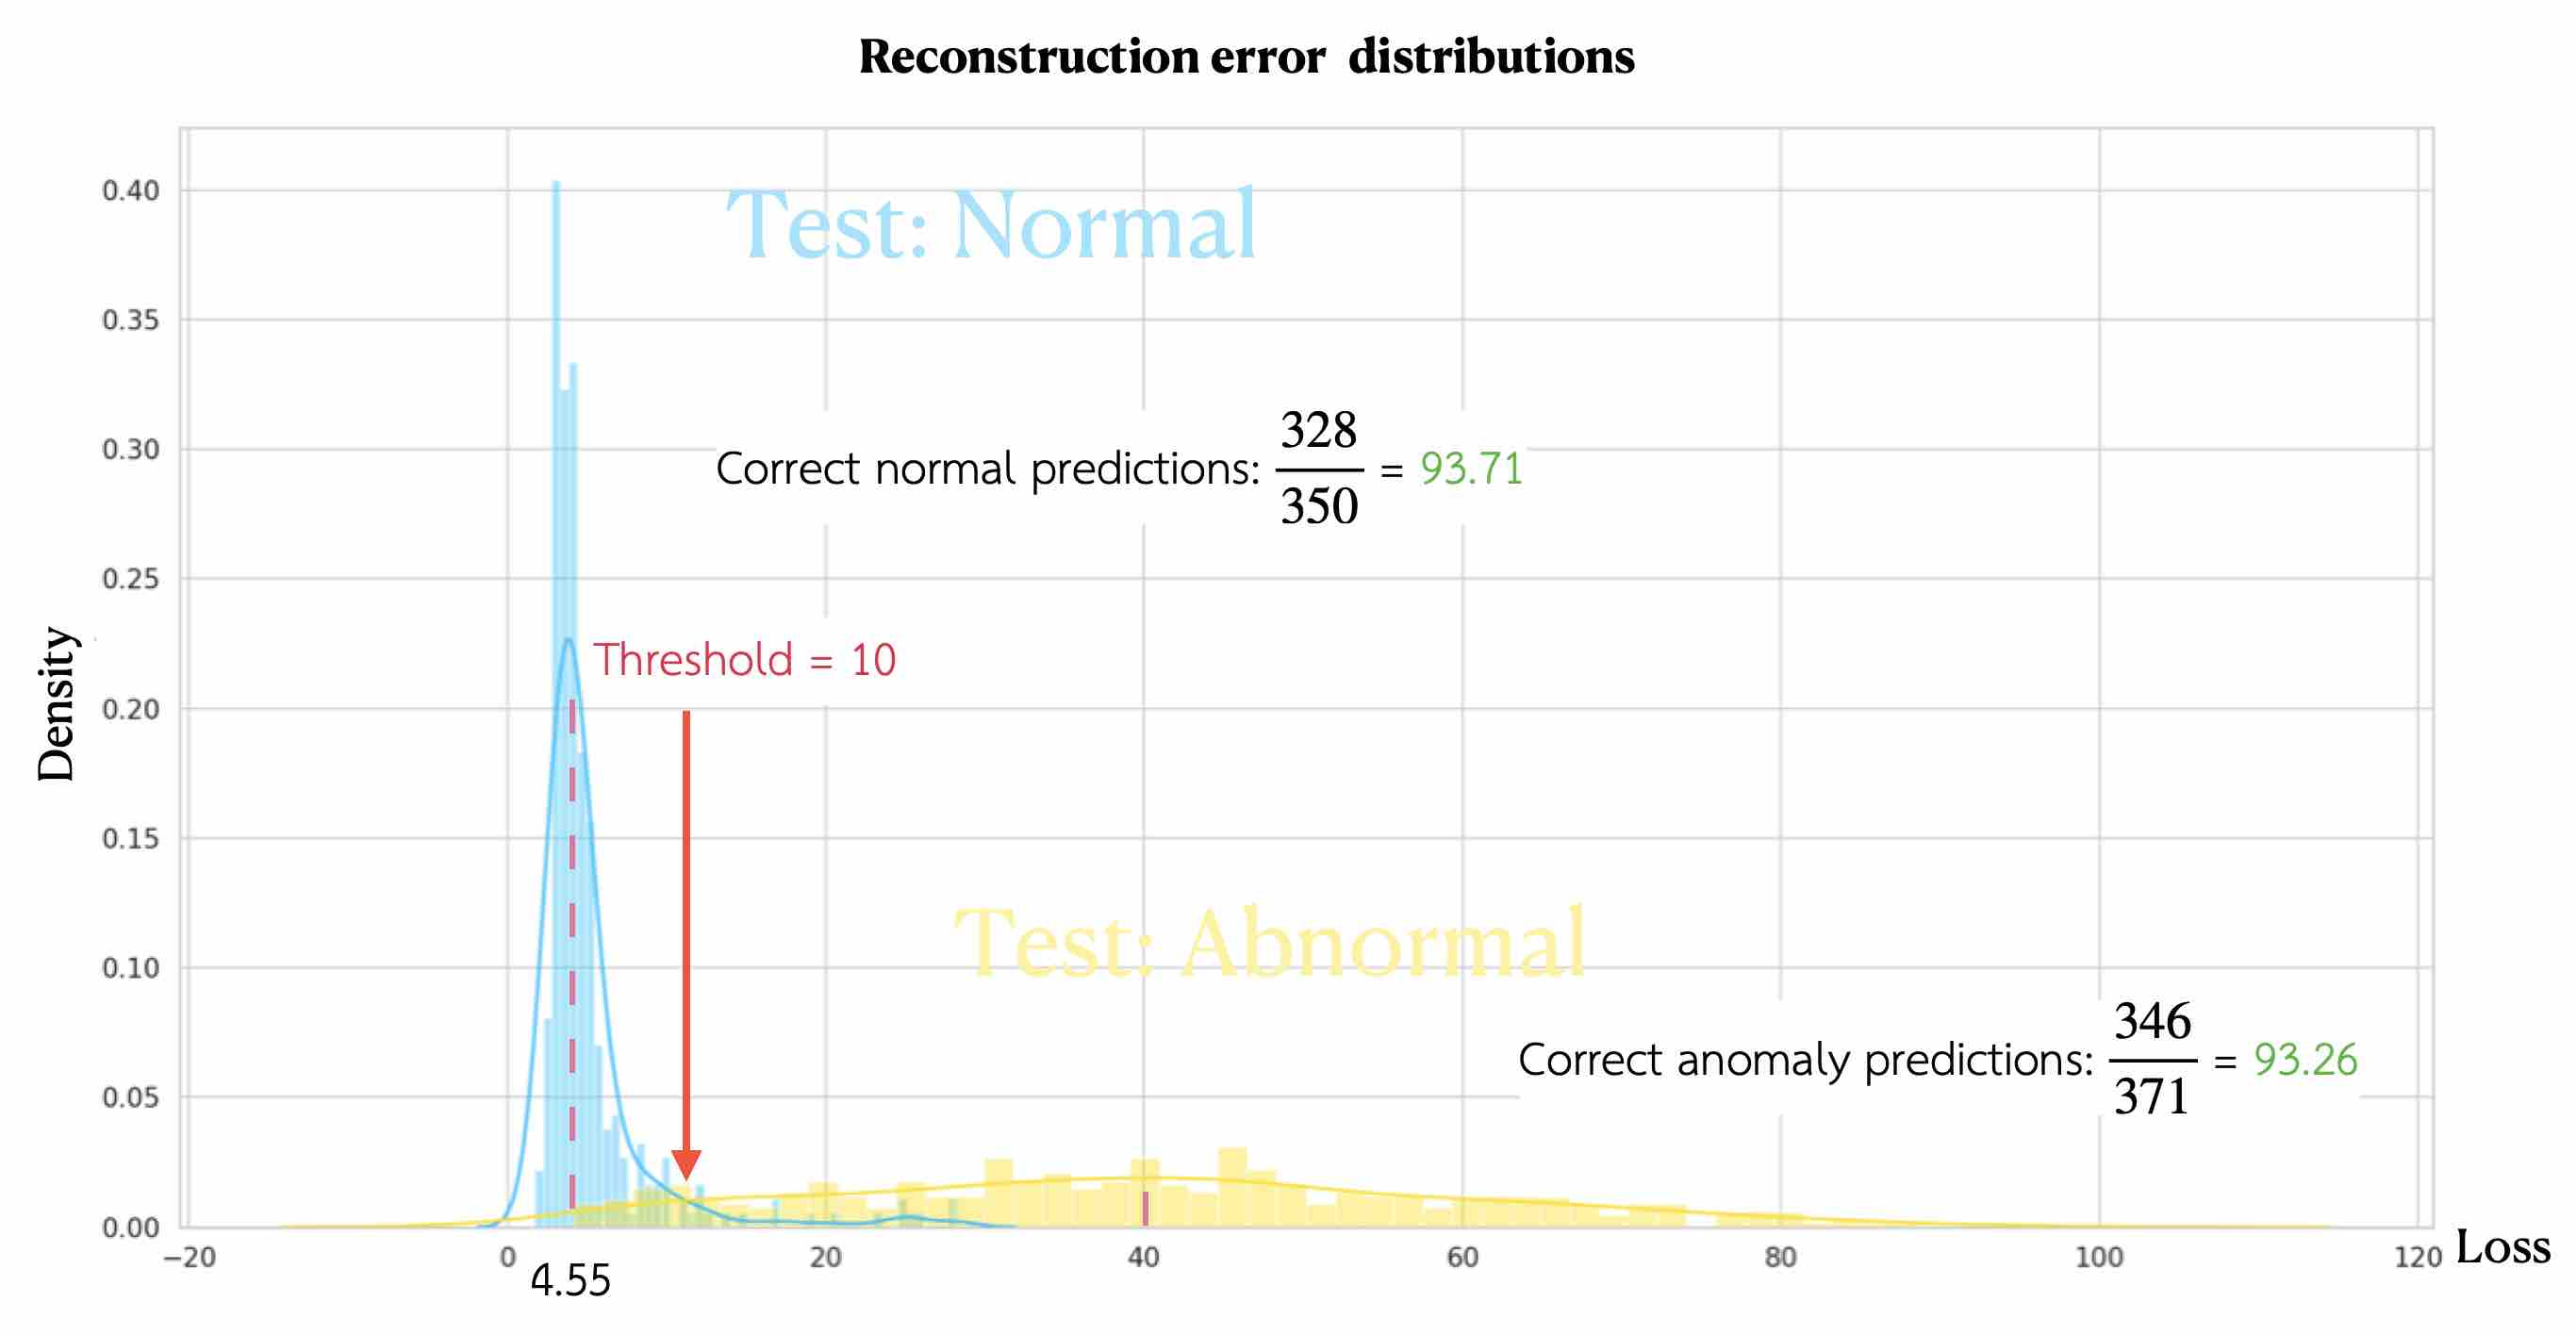
\includegraphics[scale = 0.18]{figures/autoencoder_cnnlstm_outcome.jpg}
\end{figure}

\begin{figure}[H]
  \centering
  \caption[Reconstruction data of normal and abnormal activities using 1DCNN + LSTM autoencoder.]{\emph{Reconstruction data of normal and abnormal activities using 1DCNN + LSTM autoencoder.}} \label{fig:autoencoder_cnnlstm_reconstructed_data}
  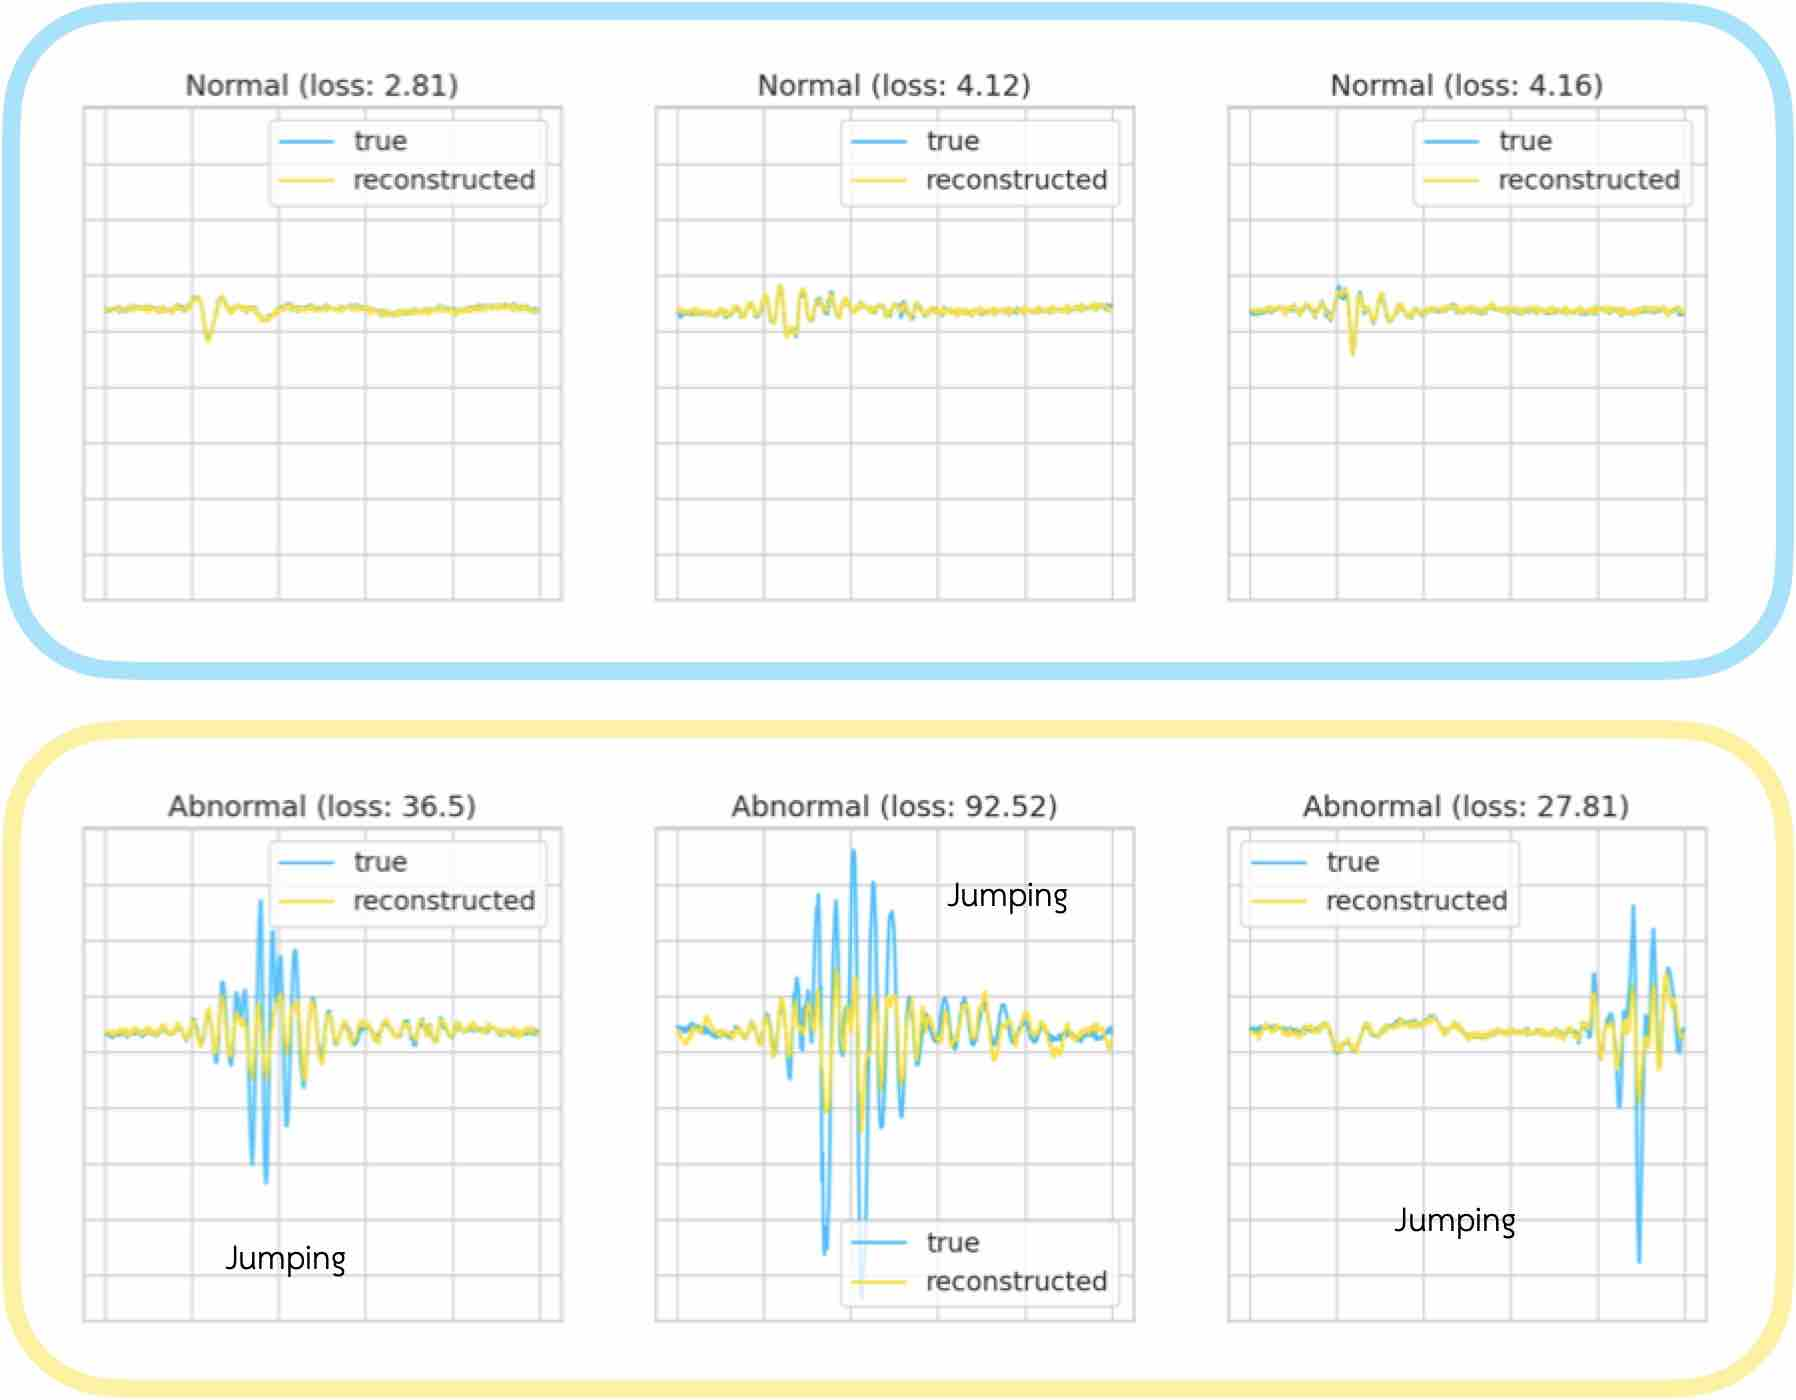
\includegraphics[scale = 0.22]{figures/autoencoder_cnnlstm_reconstructed_data.jpg}
\end{figure}


\subsection{Transformer}
The Transformer model has three encoder modules and three decoder modules. We set the number of expected features in the encoder and decoder inputs to be 128. We added a fully connected neural network of three layers (64, 32 and 1) to transform the output to one feature. The reconstructed outputs were to the first decoder module in order to predict the output at the next position as well. This model requires approximately six minutes per epoch, of training which is the longest off all the models. The adjusted hyperparameters are the number of modules, the structure of the feedforward neural network and the number of head as shown in Table \ref{tab:tran1t}, \ref{tab:tran2t}, and \ref{tab:tran3t}. Figure \ref{fig:transformer_outcome} shows the reconstruction error distributions for the test set. The distribution of the loss for the normal and abnormal activities are approximately normal with means of 13.94 and 46.40. In addition, the standard deviation of the normal activities loss is less than that of the abnormal activities, which means the model learned the normal activities fairly well. When we set the anomaly detection threshold to 19, we obtain an accuracy 89.43$\%$ for normal activities and 94.61$\%$ for abnormal activities, giving a 93.99$\%$ precision and 91.62$\%$ F1 score. Reconstructions of normal and abnormal activities are shown in Figure \ref{fig:transformer_reconstructed_data}. The reconstructiona are similar to the input for normal activities, but as expected, the model fails to reconstruct abnormal activities as accurately.

\begin{table}[H]
  \begin{center}
    \caption[Adjusting number of modules in encoder and decoder.]{\emph{Adjusting number of modules in encoder and decoder.} \hspace{\textwidth}}\label{tab:tran1t}
    \begin{tabular}{c c c c c c c}
      \hline
      \multicolumn{2}{c}{\multirow{2}{*}{\textbf{Dimension model}}} & \multicolumn{4}{c}{\textbf{Accuracy (\%)}} & \multirow{2}{*}{\textbf{Threshold}}                                                        \\
      \cline{3-6}
                                                                    &                                            & Normal events                       & Abnormal events & Precision & F1                   & \\
      \hline
      \multicolumn{2}{c}{  64 }                                     & 91.71                                      & 92.99                               & 92.51           & 92.11     & * Cannot reconstruct   \\
      \multicolumn{2}{c}{ 128 }                                     & 91.14                                      & 93.80                               & 93.27           & 92.20     & * Cannot reconstruct   \\
      \multicolumn{2}{c}{ 256 }                                     & 89.43                                      & 94.61                               & 93.99           & 91.65     & 19                     \\
      \multicolumn{2}{c}{ 512 }                                     & 90.57                                      & 92.45                               & 91.88           & 91.22     & 20                     \\
      \hline
    \end{tabular}
  \end{center}
\end{table}

\begin{table}[H]
  \begin{center}
    \caption[Adjusting structure of feedforward network.]{\emph{Adjusting structure of feedforward network.}
      \hspace{\textwidth}}\label{tab:tran2t}
    \begin{tabular}{c c c c c c c}
      \hline
      \multicolumn{2}{c}{\multirow{2}{*}{\textbf{Dimension feedforward}}} & \multicolumn{4}{c}{\textbf{Accuracy (\%)}} & \multirow{2}{*}{\textbf{Threshold}}                                      \\
      \cline{3-6}
                                                                          &                                            & Normal events                       & Abnormal events & Precision & F1 & \\
      \hline
      \multicolumn{2}{c}{  2 }                                            & 85.14                                      & 94.34                               & 93.42           & 89.09     & 18   \\
      \multicolumn{2}{c}{  4 }                                            & 86.00                                      & 93.34                               & 93.48           & 89.58     & 15   \\
      \multicolumn{2}{c}{  8 }                                            & 89.43                                      & 94.61                               & 93.99           & 91.65     & 19   \\
      \multicolumn{2}{c}{ 16 }                                            & 88.86                                      & 92.99                               & 92.28           & 90.54     & 18   \\
      \hline
    \end{tabular}
  \end{center}
\end{table}


\begin{table}[H]
  \begin{center}
    \caption[Adjusting number of Transformer heads.]{\emph{Adjusting number of Transformer heads.} \\ \hspace{\textwidth}}\label{tab:tran3t}
    \begin{tabular}{c c c c c c c}
      \hline
      \multicolumn{2}{c}{\multirow{2}{*}{\textbf{Number of head}}} & \multicolumn{4}{c}{\textbf{Accuracy (\%)}} & \multirow{2}{*}{\textbf{Threshold}}                                                        \\
      \cline{3-6}
                                                                   &                                            & Normal events                       & Abnormal events & Precision & F1                   & \\
      \hline
      \multicolumn{2}{c}{  64 }                                    & 91.71                                      & 92.99                               & 92.51           & 92.11     & * Cannot reconstruct   \\
      \multicolumn{2}{c}{ 128 }                                    & 91.14                                      & 93.80                               & 93.27           & 92.20     & * Cannot reconstruct   \\
      \multicolumn{2}{c}{ 256 }                                    & 89.43                                      & 94.61                               & 93.99           & 91.65     & 19                     \\
      \multicolumn{2}{c}{ 512 }                                    & 90.57                                      & 92.45                               & 91.88           & 91.22     & 20                     \\
      \hline
    \end{tabular}
  \end{center}
\end{table}

\begin{figure}[H]
  \centering
  \caption[Transformer reconstruction error distributions.]{\emph{Transformer reconstruction error distributions.}} \label{fig:transformer_outcome}
  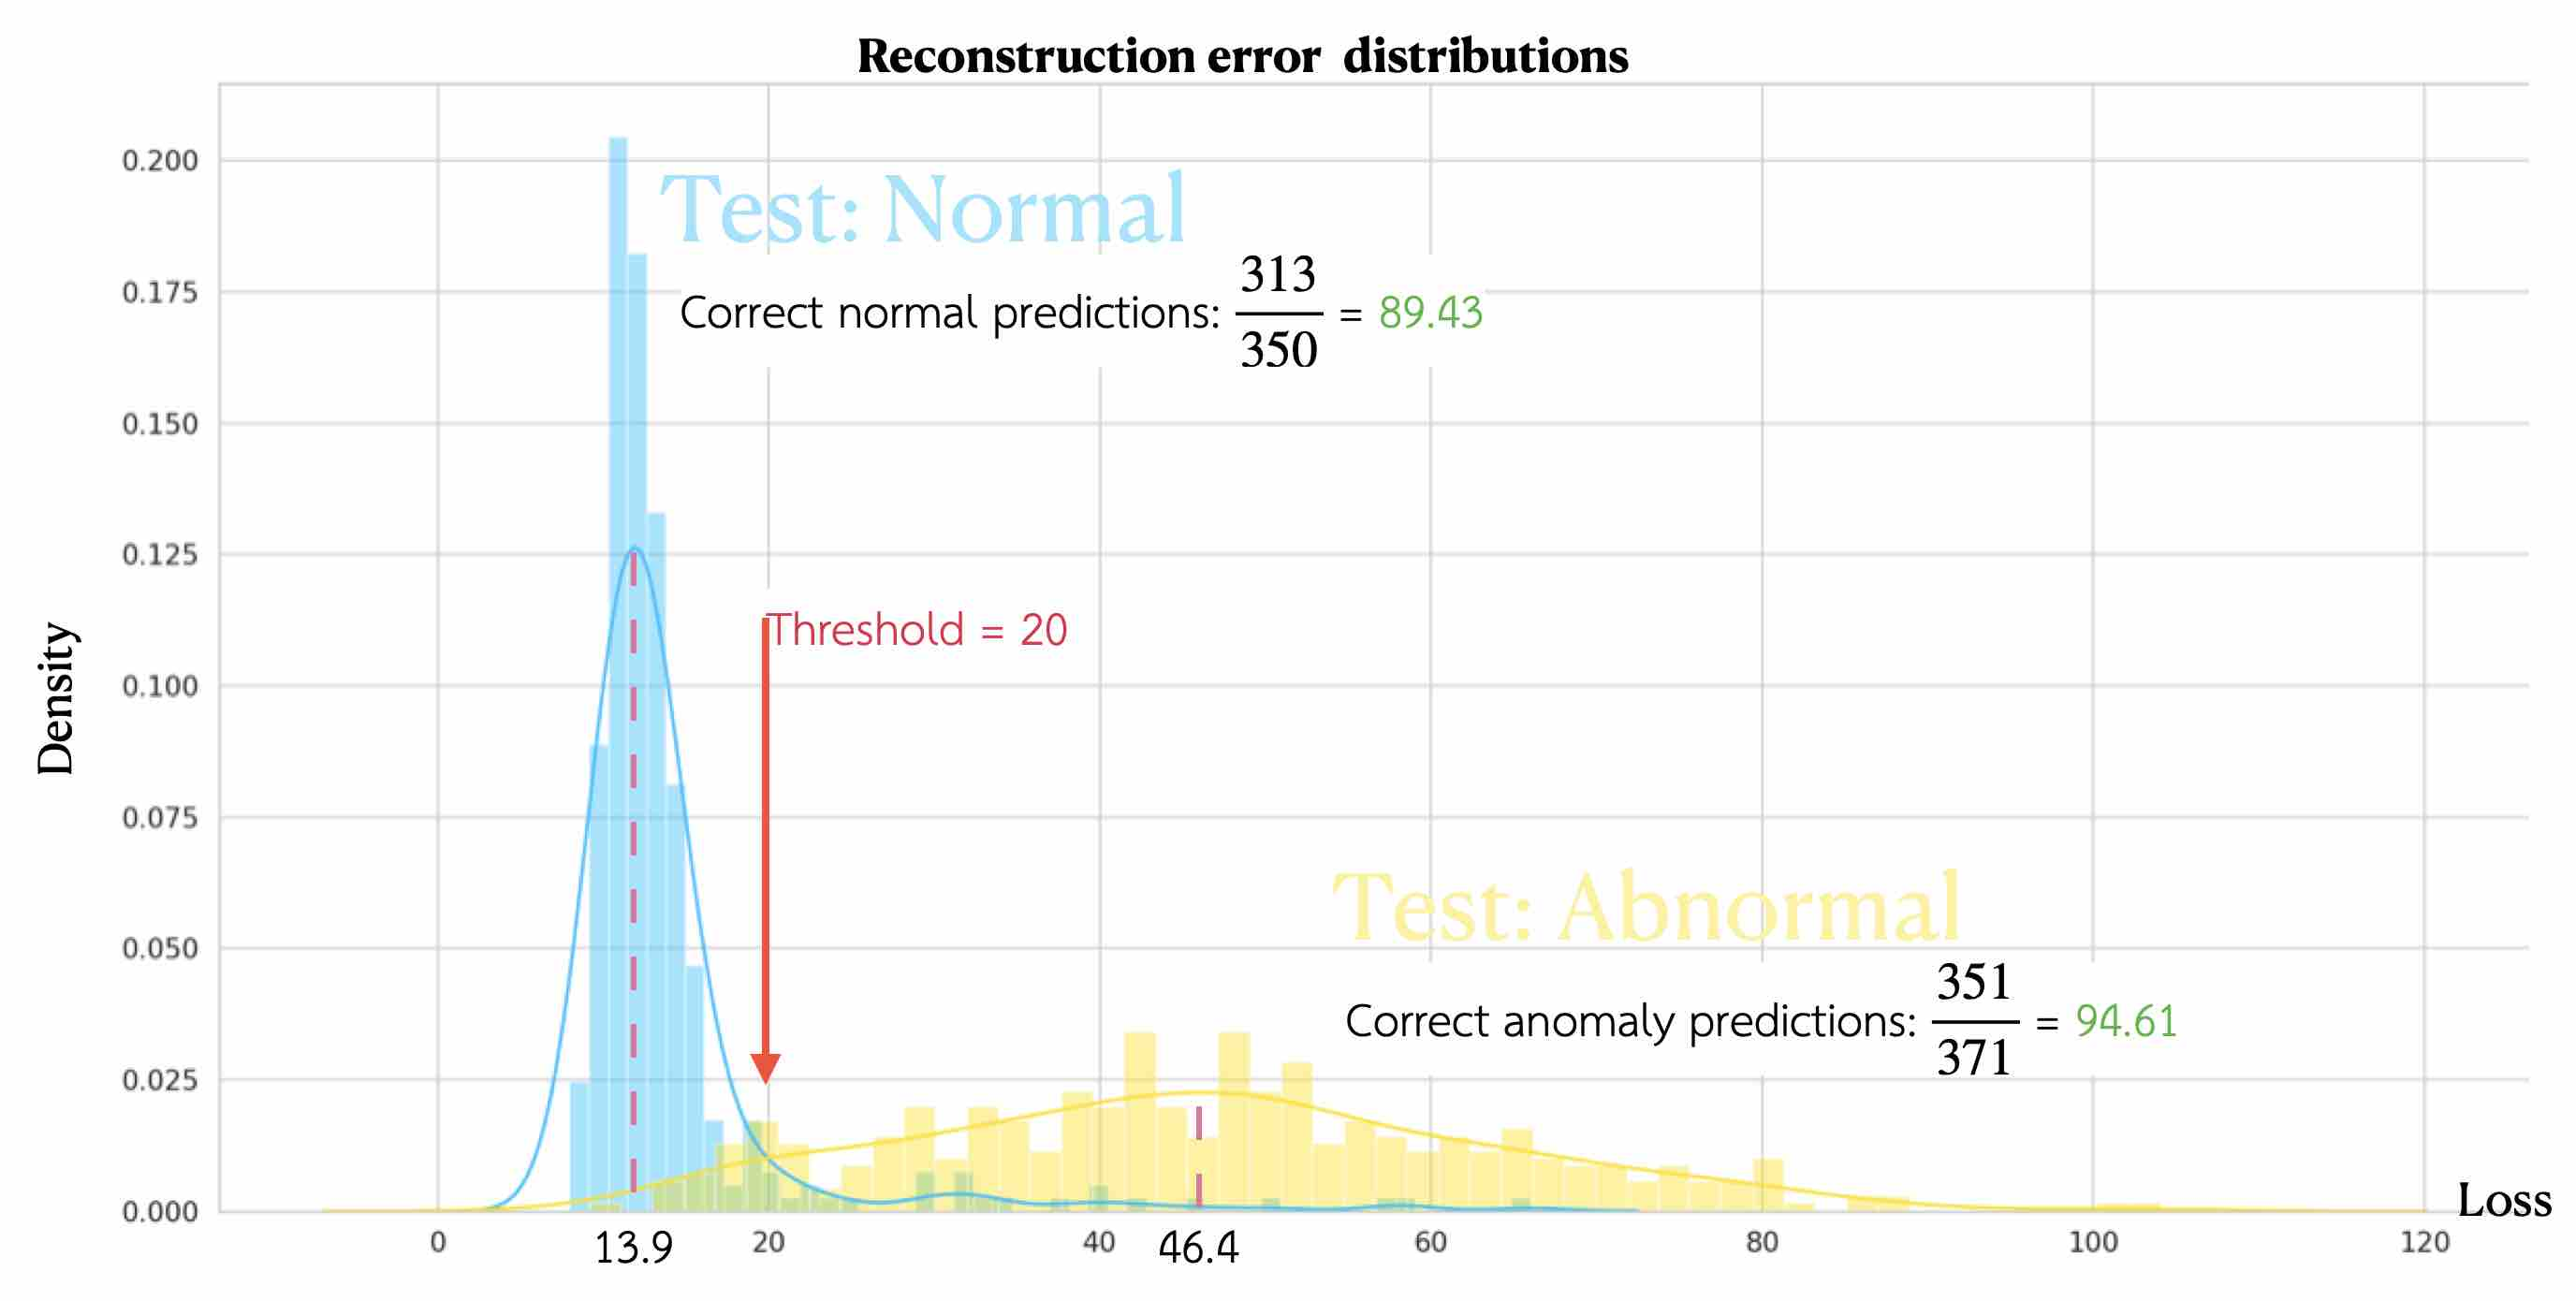
\includegraphics[scale = 0.16]{figures/transformer_outcome.jpg}
\end{figure}

\begin{figure}[H]
  \centering
  \caption[Reconstruction normal and abnormal activities using Transformer.]{\emph{Reconstruction normal and abnormal activities using Transformer.}} \label{fig:transformer_reconstructed_data}
  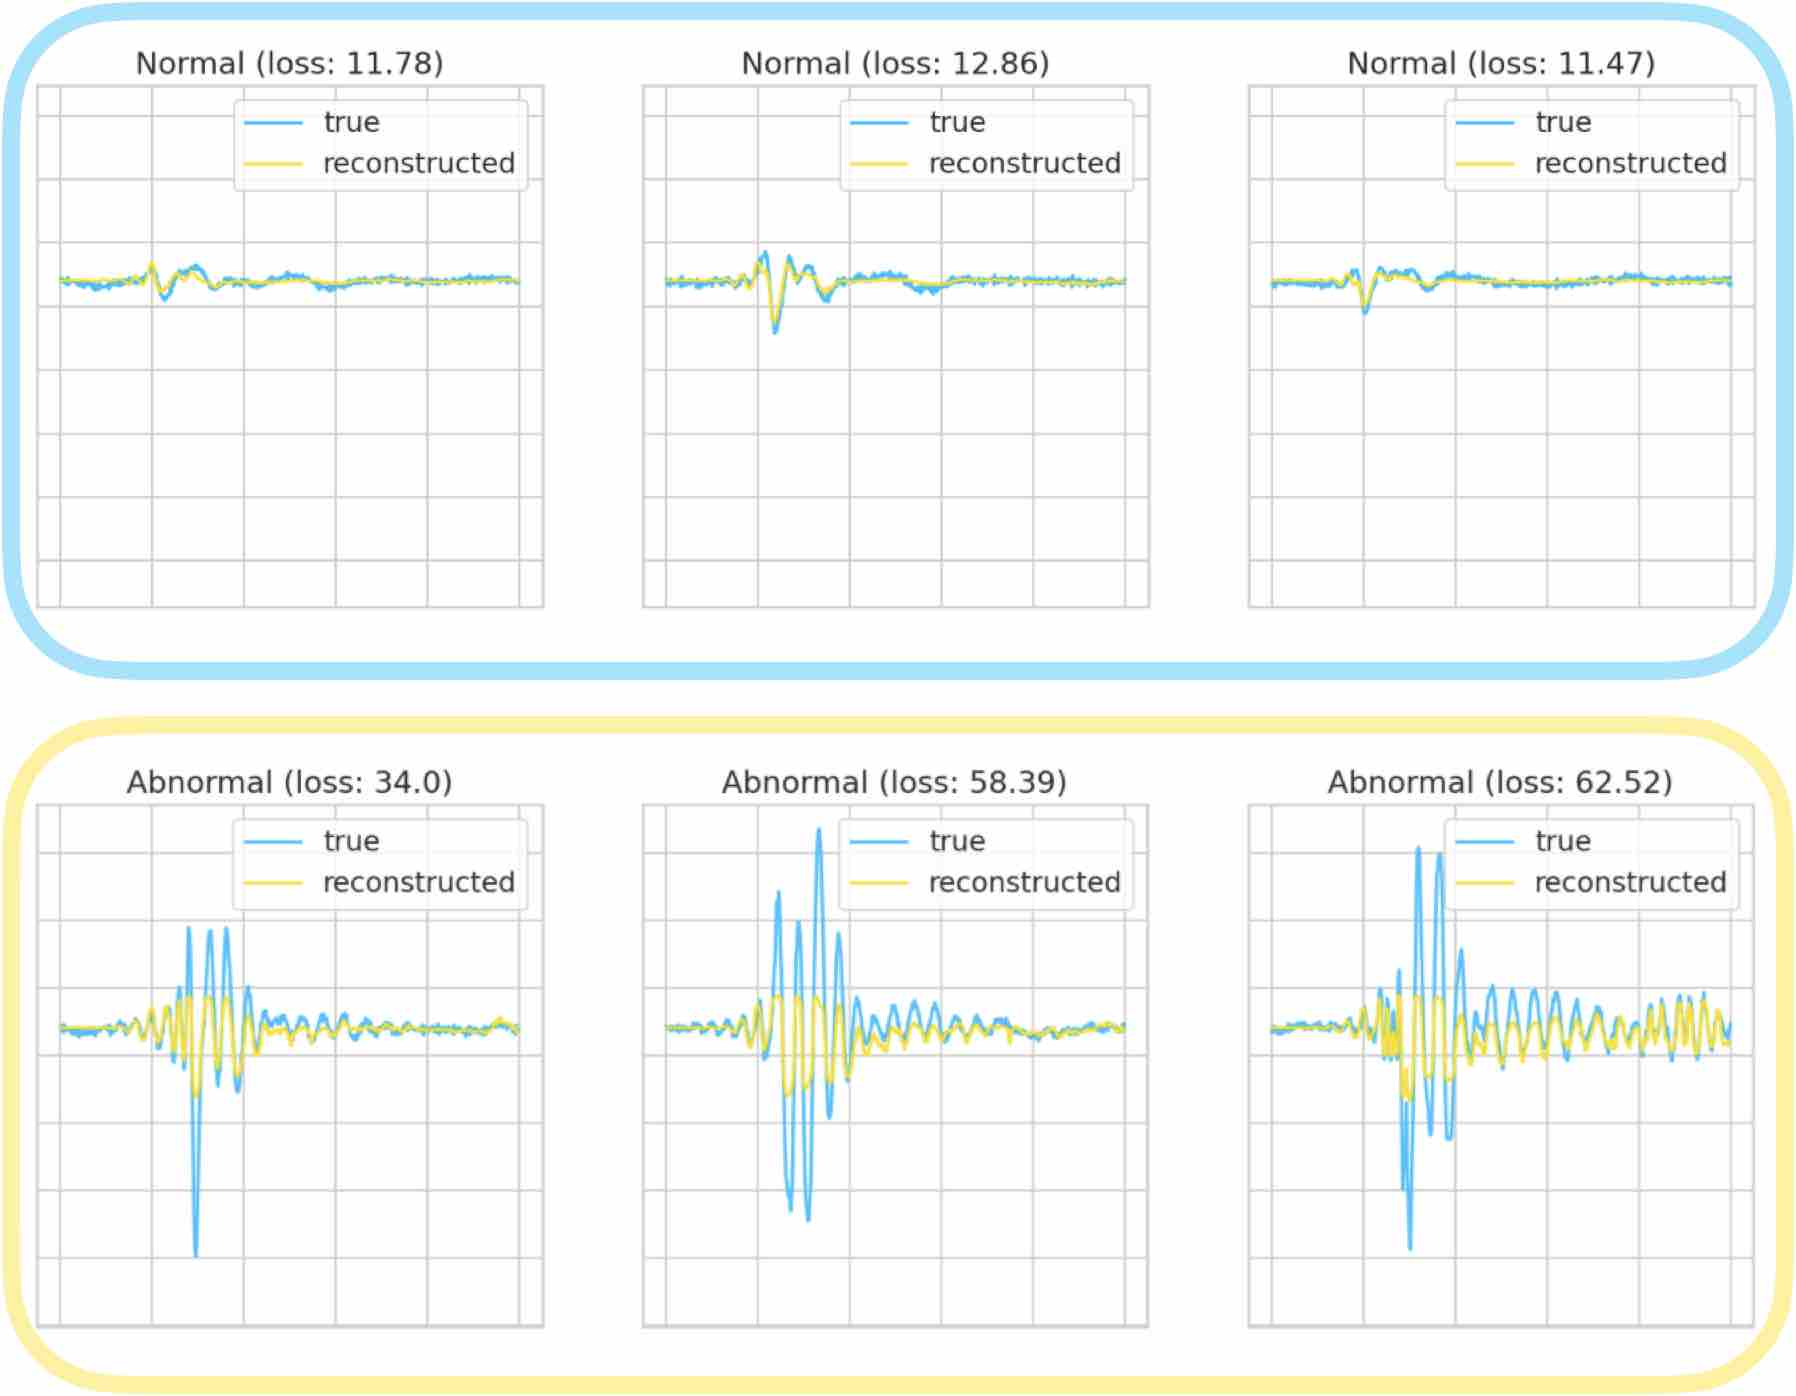
\includegraphics[scale = 0.22]{figures/transformer_reconstructed_data.jpg}
\end{figure}

\subsection{Principal Components Analysis}
We built separate models with the number of components from 1 -- 49 with an anomaly detection threshold from -5000 to 5000. Results are shown in Figure \ref{fig:pca-f1}. The best F1 score belonged to the model with one component, 94.22$\%$. When we set the anomaly detection threshold to 500, we obtain an accuracy 90.86$\%$ for normal activities and 98.11$\%$ for abnormal activies, giving has 97.85$\%$ precision. A visualization of results on the test set is shown in Figure \ref{fig:pca-outcome}.

\begin{figure}[H]
  \centering
  \caption[F1 score as a function of number of principal components.]{\emph{F1 score as a function of number of principal components.}} \label{fig:pca-f1}
  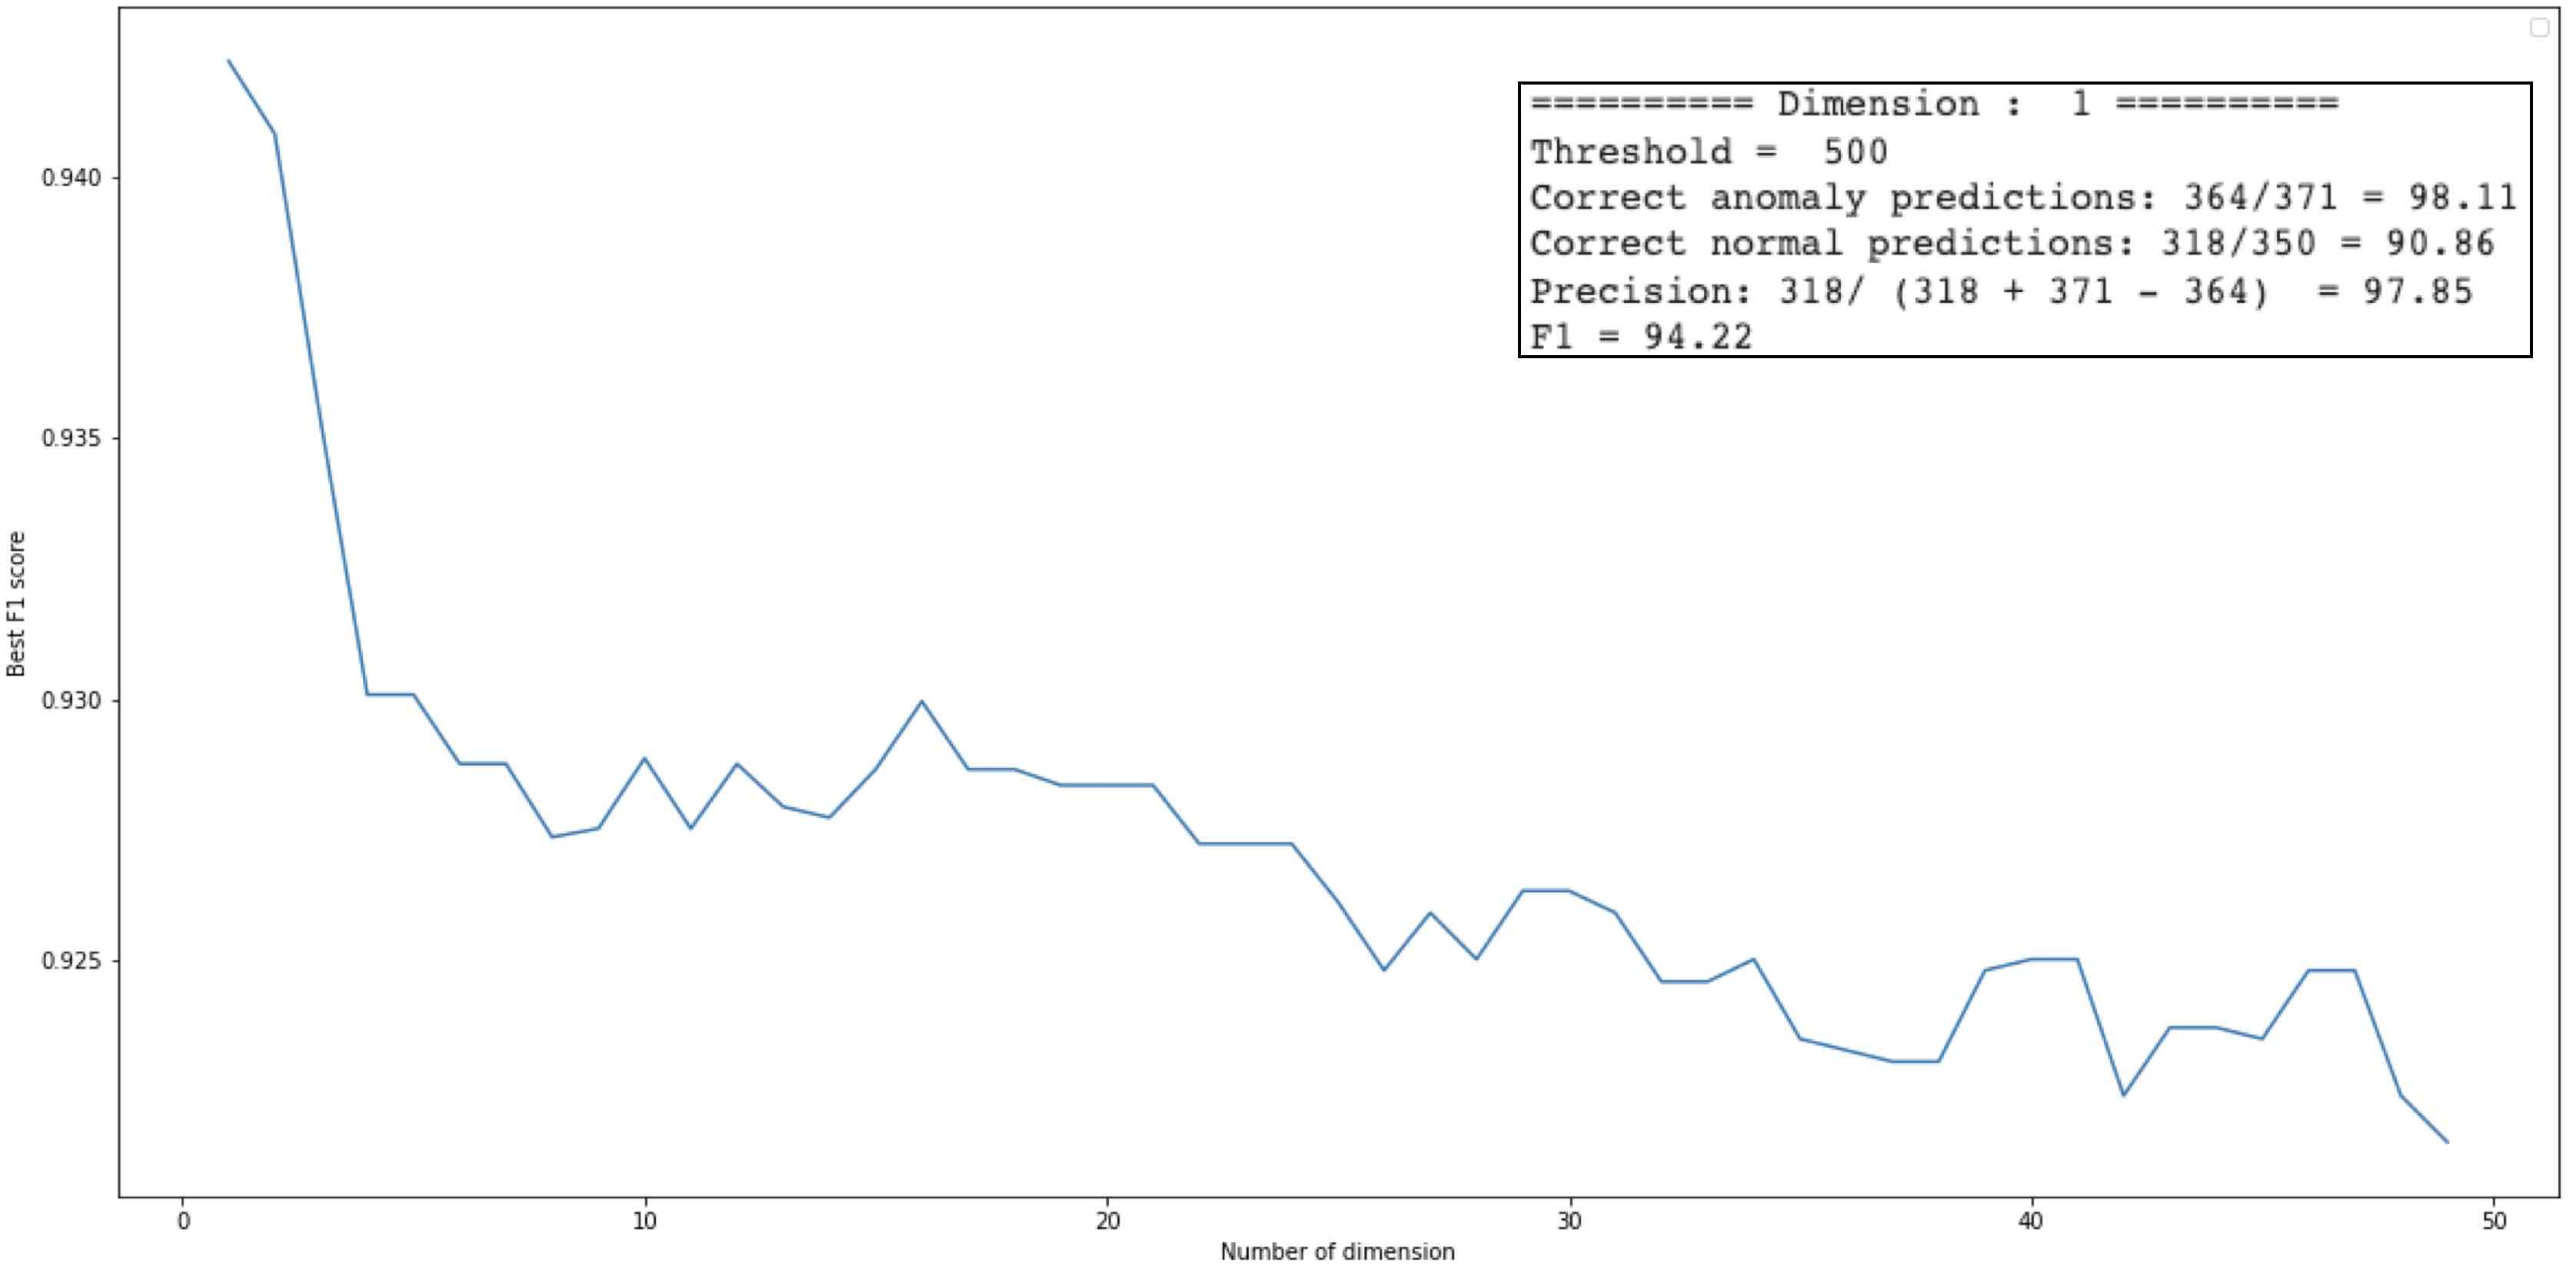
\includegraphics[scale = 0.13]{figures/pca-f1.jpg}
\end{figure}

\begin{figure}[H]
  \centering
  \caption[The outcome of PCA in test set.]{\emph{The outcome of PCA in test set.}} \label{fig:pca-outcome}
  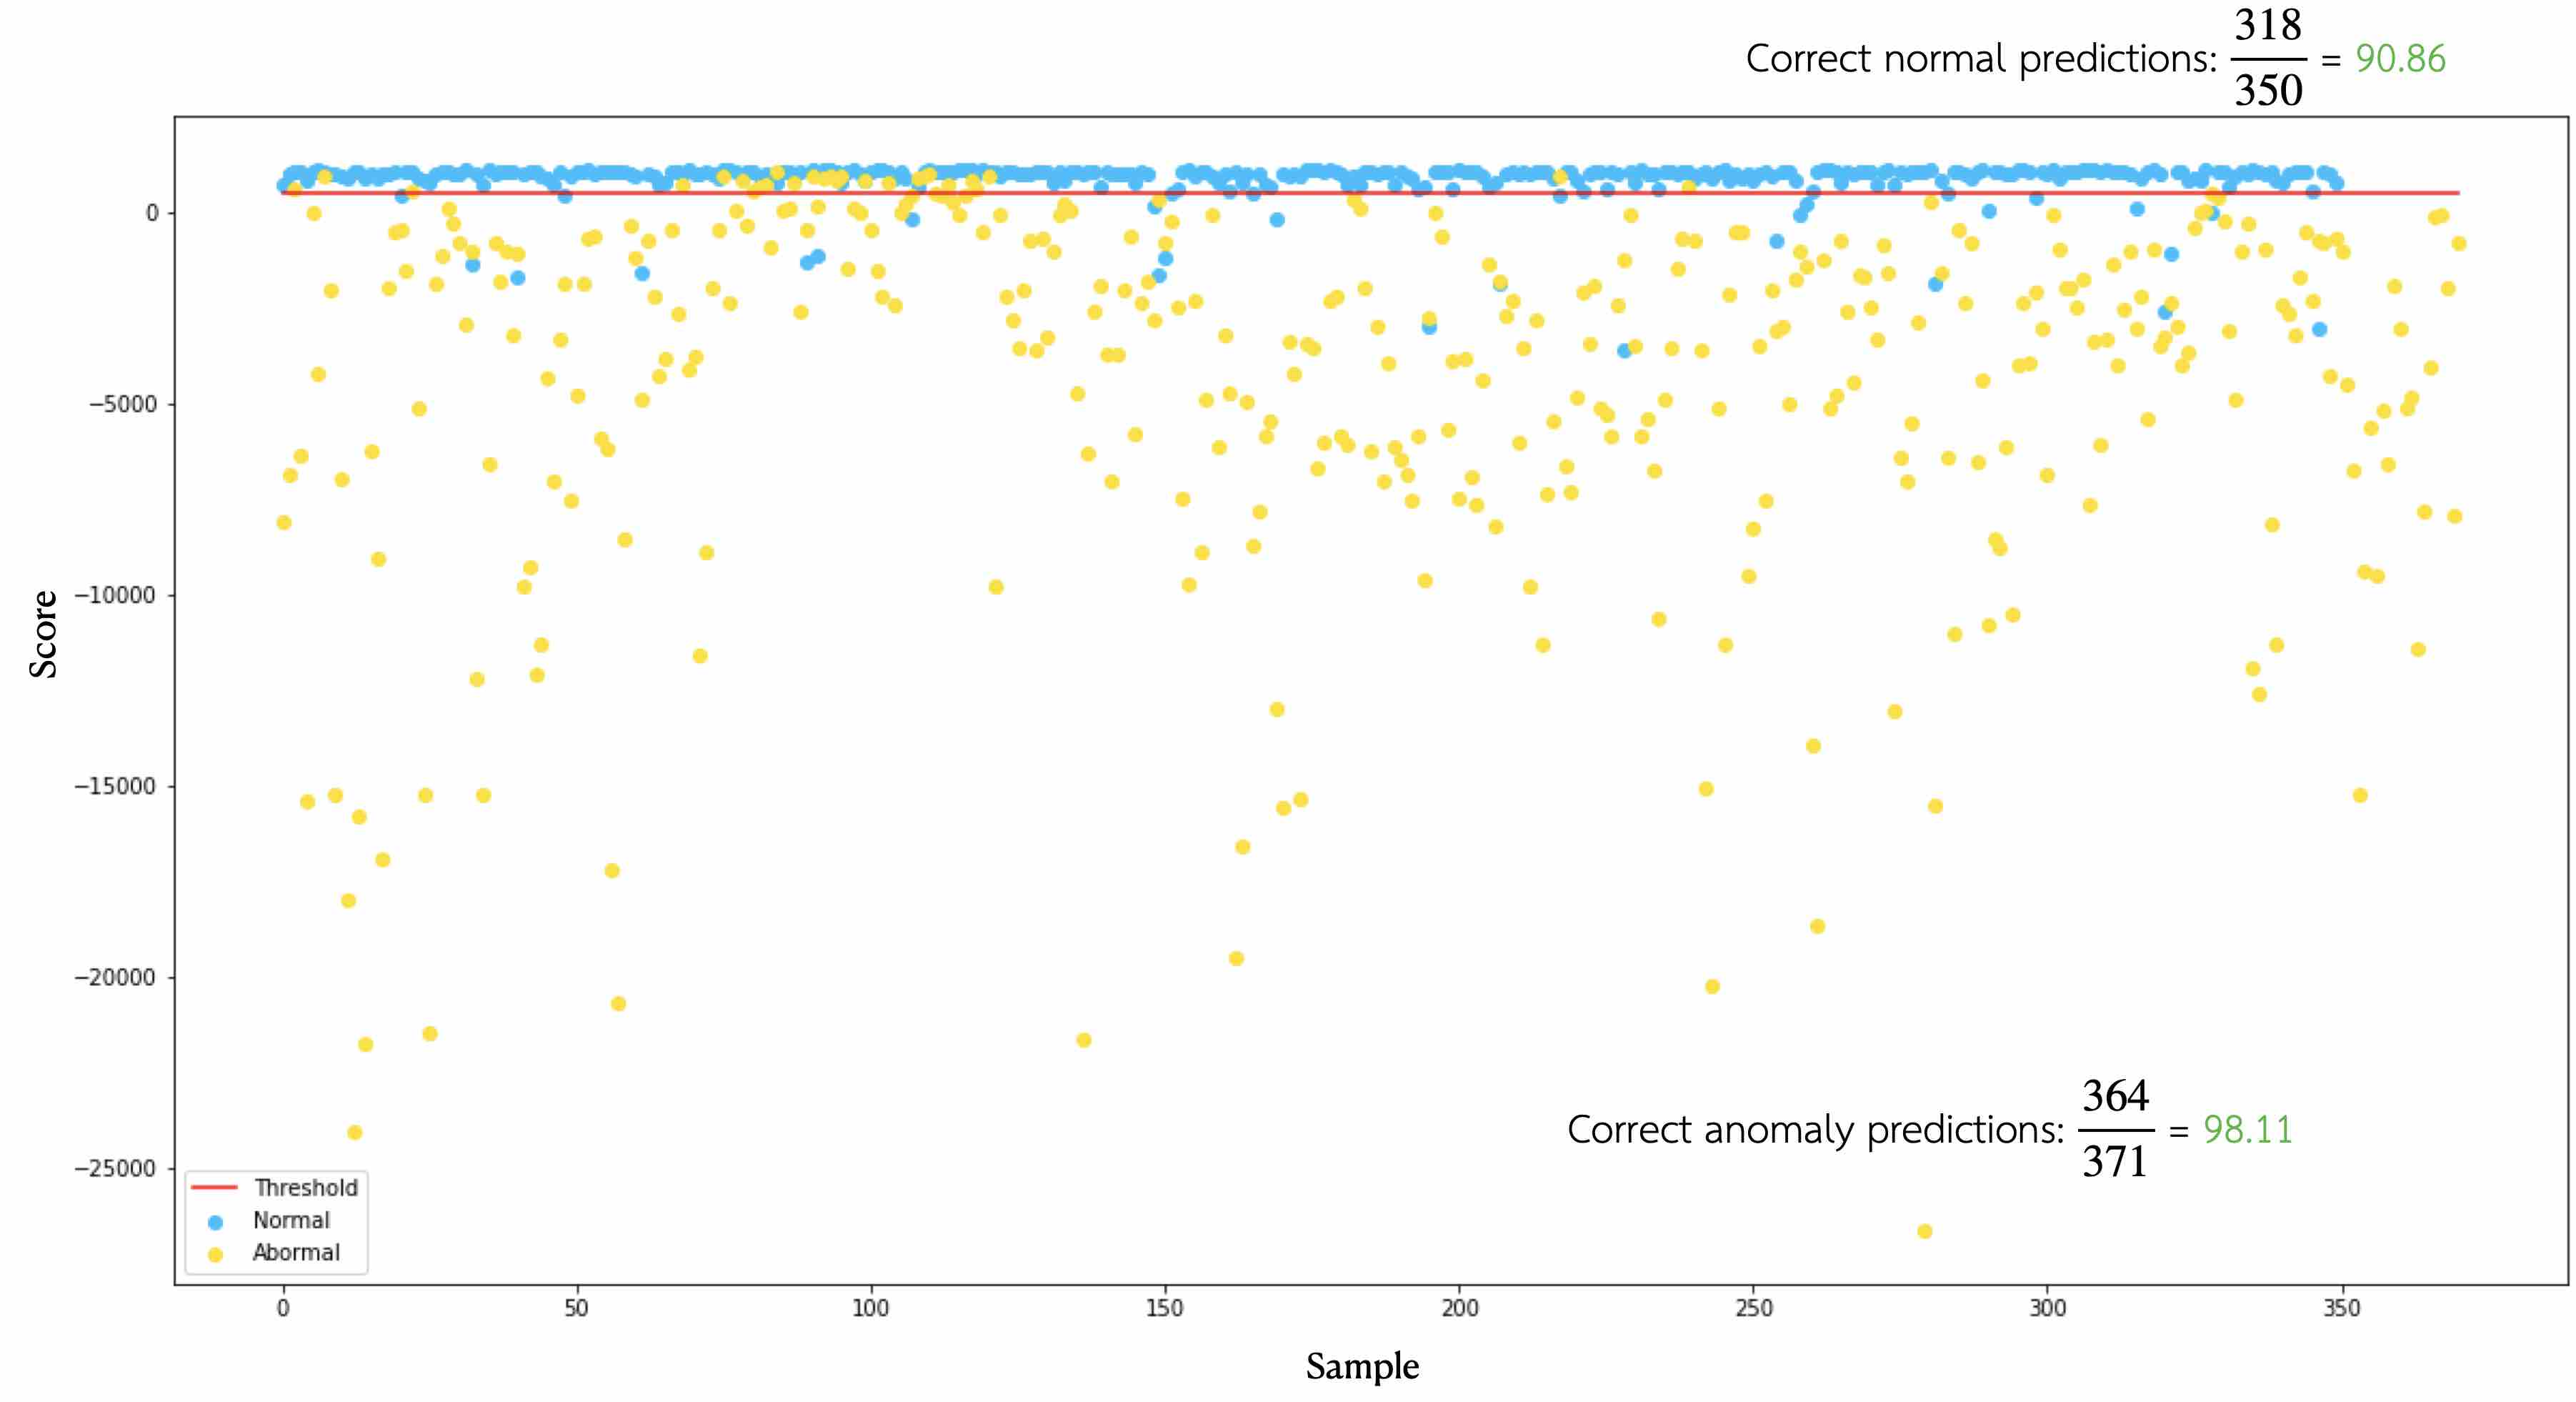
\includegraphics[scale = 0.13]{figures/pca_outcome.jpg}
\end{figure}

\subsection{Model summary}
A summay of the best version of each model based on this dataset is given in Table \ref{tab:modelsum}. It seems that PCA provides the best F1 score among all models. PCA also requires the least amount of time for a prediction, making it highly suitable for predicting the event in real time. Consequently, we select PCA for the final deployment experiments.

\begin{table}[H]
  \begin{center}
    \caption[Model summary.]{\emph{Model summary.} \\ \hspace{\textwidth}}\label{tab:modelsum}
    \begin{tabular}{c c c c c c c}
      \hline
      \multicolumn{2}{c}{\multirow{2}{*}{\textbf{Model}}} & \multicolumn{4}{c}{\textbf{Accuracy (\%)}} & \multirow{2}{*}{\textbf{Training time}}                                                 \\
      \cline{3-6}
                                                          &                                            & Normal events                           & Abnormal events & Precision & F1            & \\
      \hline
      \multicolumn{2}{c}{  LSTM Autoencoder }             & 89.08                                      & 93.00                                   & 89.07           & 89.07     & 280 s / epoch   \\
      \multicolumn{2}{c}{ CNN Autoencoder }               & 94.00                                      & 92.72                                   & 92.42           & 93.20     & 13 s / epoch    \\
      \multicolumn{2}{c}{ CNN + LSTM Autoencoder }        & 93.71                                      & 93.26                                   & 92.92           & 93.31     & 100 s / epoch   \\
      \multicolumn{2}{c}{ Transformer }                   & 89.43                                      & 94.61                                   & 93.99           & 91.65     & 330 s / epoch   \\
      \multicolumn{2}{c}{ PCA }                           & 90.86                                      & 98.11                                   & 97.85           & 94.22     & 200 ms          \\
      \hline
    \end{tabular}
  \end{center}
\end{table}

\section{Deployment}
The deployed system is intended to be plug \& play. Every component, such as theseismic sensor, data acquisition module, and Raspberry Pi is integrated in a small box, dimension 13 x 19 x 7 $\mathrm{cm}^{3}$, requiring only a power adapter, as shown in Figure \ref{fig:application}. The software architecture is shown in Figure \ref{fig:software_architecture}. The program performs two tasks concurrently as reading data from the sensor and predicting every five seconds. The two tasks run as separate threads to ensure that they can run concurrently. The PCA analytic is used for the prediction task. We use an anomaly detection threshold of 500, which performed the best validation set in terms of F1 score. When anomalous activities occur, an alert message is sent via the LINE application within 5 seconds. 

\begin{figure}[H]
  \centering
  \caption[The complete application.]{\emph{The complete application.}} \label{fig:application}
  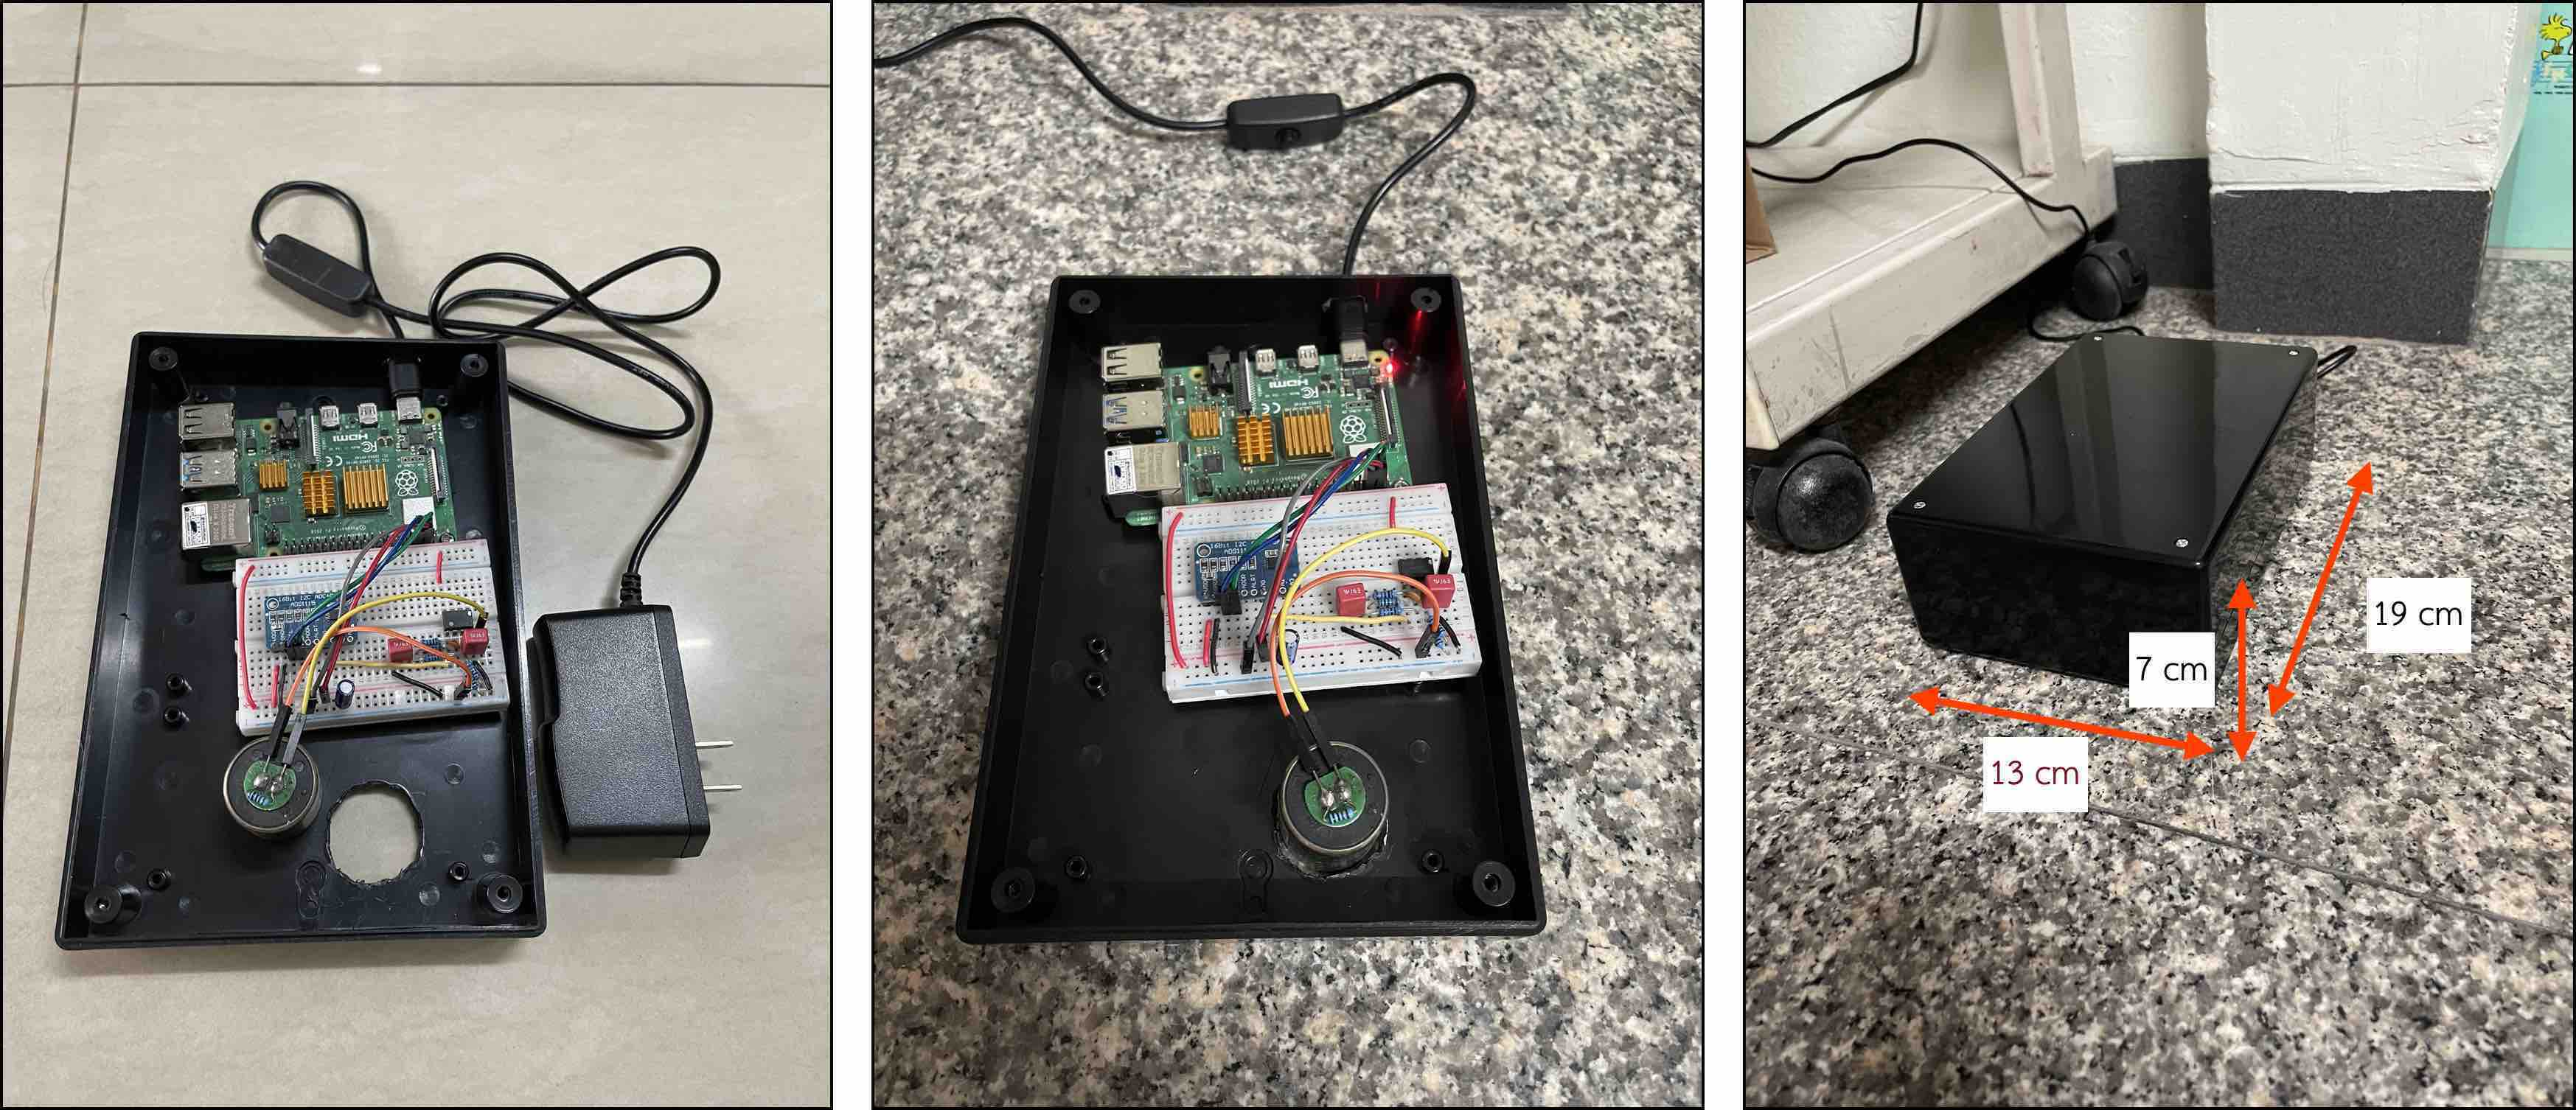
\includegraphics[scale = 0.14]{figures/application.jpg}
\end{figure}

\begin{figure}[H]
  \centering
  \caption[Data reader and inference engine run their own threads.]{\emph{Data reader and inference engine run their own threads.}} \label{fig:software_architecture}
  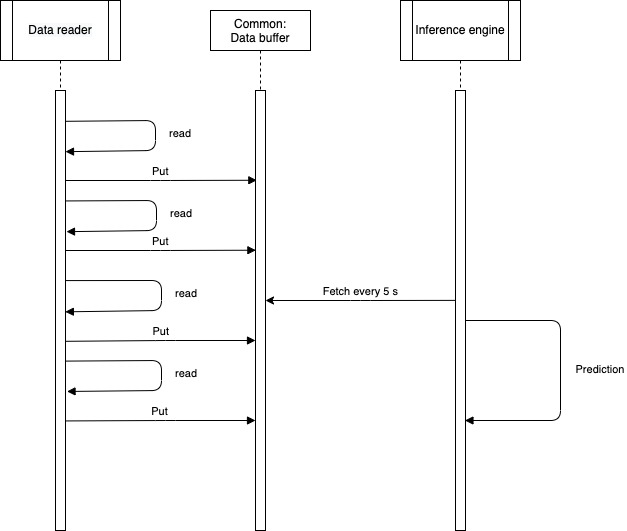
\includegraphics[scale = 0.7]{figures/software_architecture.jpg}
\end{figure}

We deployed this system on 9 March, 2022 for 12 hours, 12:00 pm to 0:00 am. During this time, we performed ordinary activities similar to any the other day. The timeline of deployment and the event that occurred are shown in Figure \ref{fig:timelinedeploy}. There are totally 929 detected events and 32 alerts message. The first notice occurred when there was more than one human in the room, e.g. at 3-4 pm and 6-7 pm. The system has approximately six false alarms, during these times. Otherwise, the sensor performed very well at detecting anomalous events. To test detection of abnormal event, we performed several anomalous events such as jumping and dropping a water bottle as well as simulating falls. In terms of accuracy, we obtain 98.46$\%$ accuracy for normal activities and 90.00$\%$ for anomalous activities. A summary of deployed experientment is shown in Figure \ref{fig:summarydeploy}. A video is posted at \url{https://youtu.be/OU6DYq9JNZw}.

\begin{figure}[H]
  \centering
  \caption[Timeline of deployment experientment.]{\emph{Timeline of deployment experientment.}}  \label{fig:timelinedeploy}
  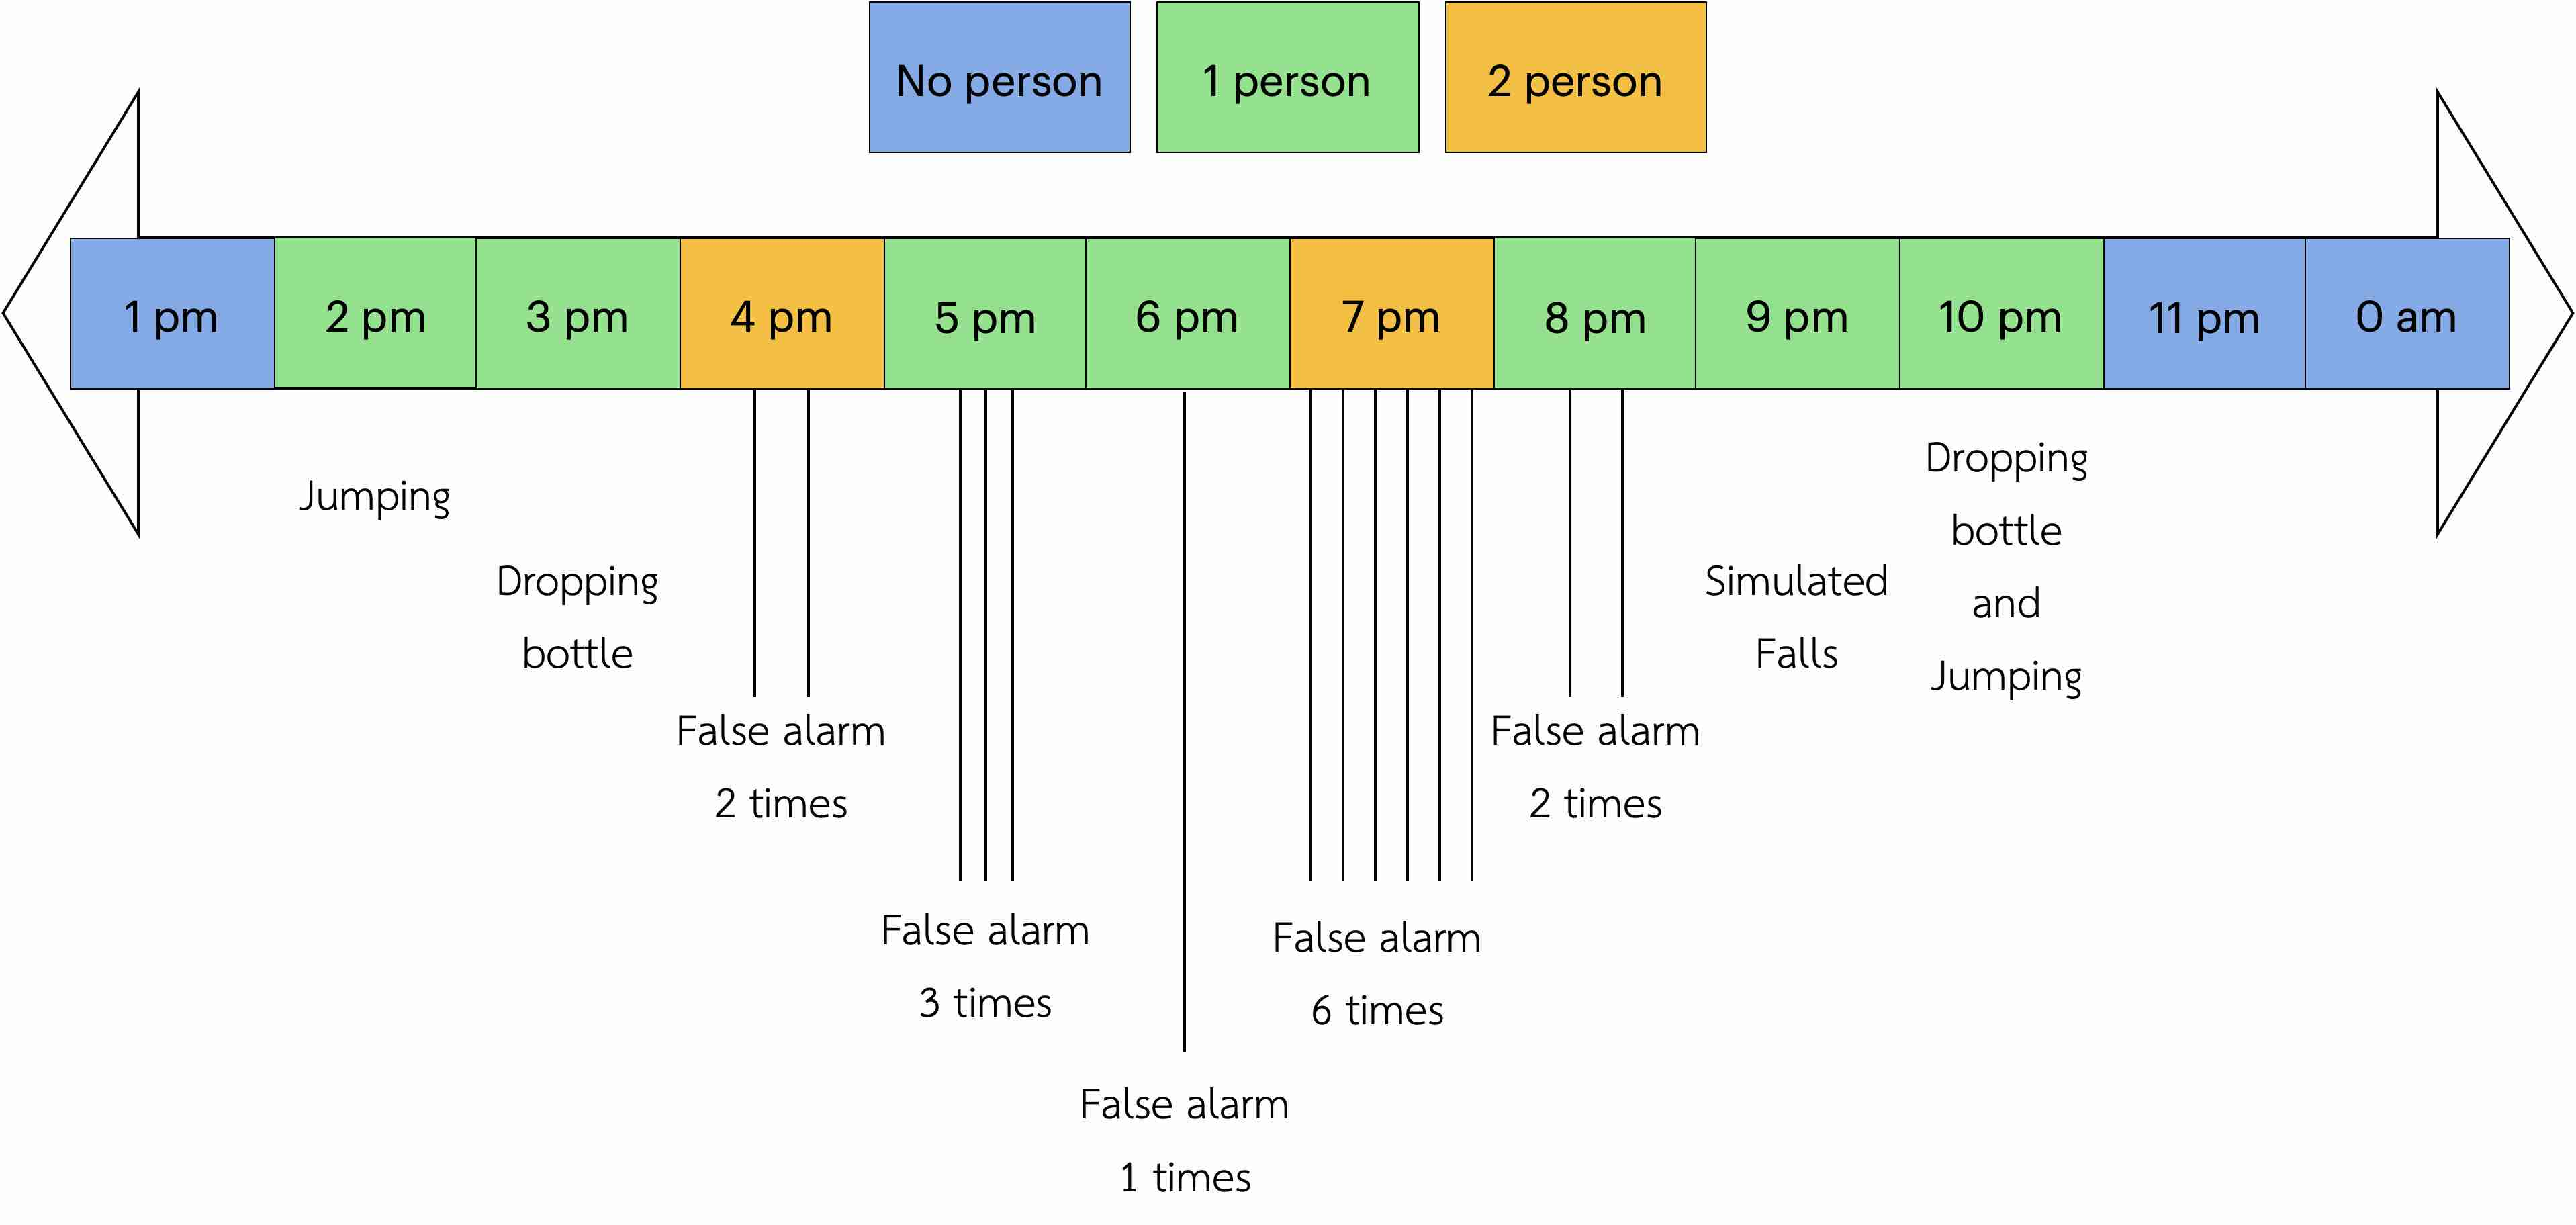
\includegraphics[scale = 0.13]{figures/timelinedeployment.jpg}
\end{figure}

\begin{figure}[H]
  \centering
  \caption[Summary of deployment experientment.]{\emph{Summary of deployment experientment.}} \label{fig:summarydeploy}
  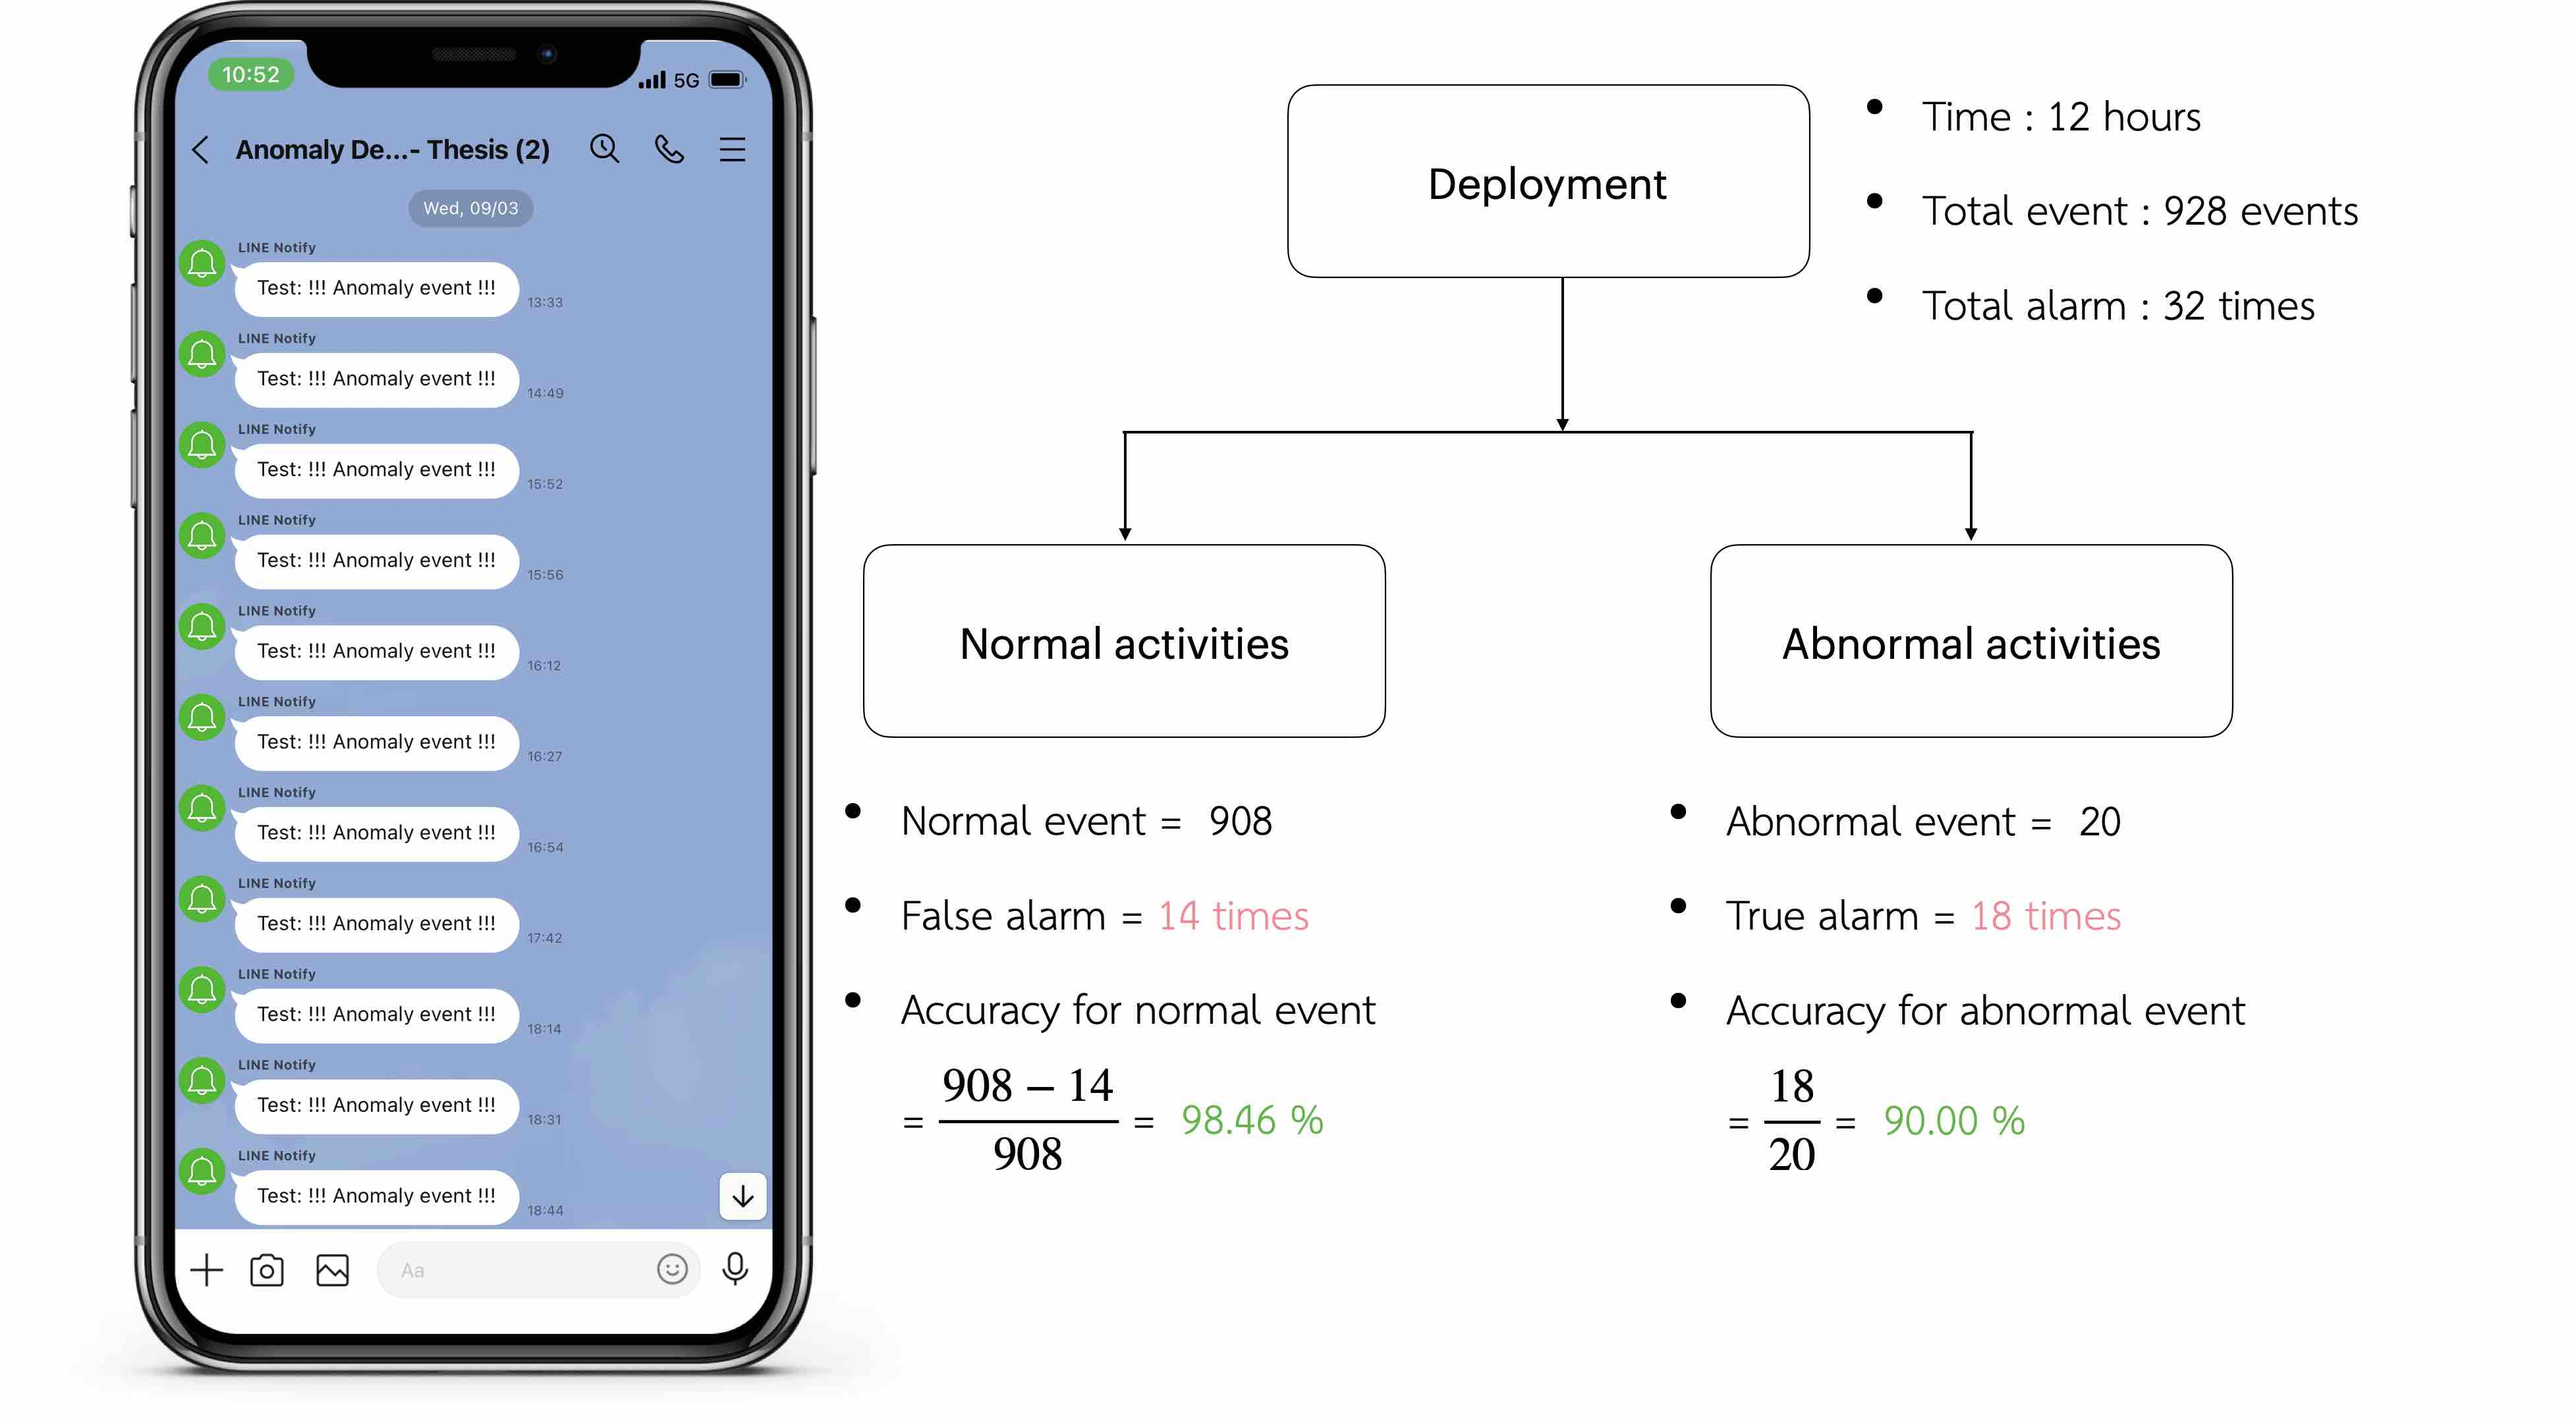
\includegraphics[scale = 0.13]{figures/summarydeployment.jpg}
\end{figure}

\FloatBarrier